\documentclass[12pt,a4paper]{extreport}
\usepackage[utf8]{inputenc}
%\usepackage[T5]{fontenc}
\usepackage[utf8]{vietnam}
\usepackage{times}
\usepackage{enumerate}
\usepackage{enumitem}
\usepackage{multicol}
\usepackage{listings}
%\usepackage[left=2cm,right=2cm,top=2.5cm,bottom=2.5cm]{geometry}
\usepackage[a4paper, top=3.5cm,bottom=3cm,left=3.5cm,right=2cm]{geometry}
\usepackage{verbatim}
\usepackage{graphicx}
\usepackage{url}
\usepackage{fancyhdr}
\usepackage{fancybox,framed}
\linespread{1.3}
\usepackage{lastpage}
\usepackage{floatrow}
\usepackage{floatrow}
\usepackage{array}
\usepackage{longtable}

\pagenumbering{arabic}
%\pagestyle{fancy}
\newfloatcommand{capbtabbox}{table}[][\FBwidth]
\usepackage{caption}
\captionsetup[figure]{font=large} 
\usepackage{blindtext}
\usepackage{titlesec}
\usepackage[nottoc]{tocbibind}
\usepackage{bookmark}

% ******************************************************************************
%\setlength{\topmargin}{-0.5cm} % Lề trên
%\setlength{\oddsidemargin}{-0.5cm} % Lề trái
%\setlength{\evensidemargin}{-0.5cm} % Lề phải
%\setlength{\textwidth}{15.5cm} % Chiều rộng văn bản
%\setlength{\textheight}{24cm} % Chiều cao văn bản
%\setlength{\footskip}{1cm} % Khoảng cách giữa nội dung và số trang

% For line spacing 1.5
%\usepackage{setspace}
%\renewcommand{\baselinestretch}{1.5}

% ******************************************************************************
\usepackage{hyperref}
% Cấu hình cho \paragraph để nó xuống hàng sau tiêu đề
\titleformat{\paragraph}[block]
{\normalfont\normalsize\bfseries}{\theparagraph}{1em}{}

\titlespacing*{\paragraph}
{0pt}{3.25ex plus 1ex minus .2ex}{1.5ex plus .2ex}

\setcounter{secnumdepth}{4}
\setcounter{tocdepth}{4}

\usepackage{array} % Gói cần thiết cho kiểu cột m{}

\titleformat*{\section}{\LARGE\bfseries}
\titleformat*{\subsection}{\Large\bfseries}
\titleformat*{\subsubsection}{\large\bfseries}
%\addbibresource{ref.bib}

\usepackage{mdframed}
\usepackage{alltt}
\usepackage{color}
\usepackage{tocloft}
\usepackage{caption}

\usepackage{tikz}
\usetikzlibrary{calc}
\fancyfoot[C]{\thepage}

% Math
\usepackage{amsfonts}


% ******************************************************************************
% Cấu trúc chương và mục
\renewcommand{\thechapter}{\arabic{chapter}} % Số chương bằng số tự nhiên
\renewcommand{\thesection}{\arabic{section}} % Số mục bằng số tự nhiên
\renewcommand{\thesubsection}{\arabic{section}.\arabic{subsection}} % Số tiểu mục
\renewcommand{\thesubsubsection}{\arabic{section}.\arabic{subsection}.\arabic{subsubsection}} % Số tiểu tiểu mục

% Đánh số hình, bảng, phương trình theo chương
\renewcommand{\thefigure}{\thechapter.\arabic{figure}} % Đánh số hình
\renewcommand{\thetable}{\thechapter.\arabic{table}} % Đánh số bảng
\renewcommand{\theequation}{\thechapter.\arabic{equation}} % Đánh số phương trình

% Tạo danh mục viết tắt
\newcommand{\acronym}[2]{\textbf{#1} (\textit{#2})}

% Tùy chỉnh tiêu đề và khoảng cách trong danh mục hình ảnh
\renewcommand{\cftfigpresnum}{Hình~} % Tiền tố trước số hình ảnh
\renewcommand{\cftfigaftersnum}{:} % Ký tự sau số hình ảnh
\addtolength{\cftfignumwidth}{3em} % Tăng khoảng cách giữa số và tiêu đề hình ảnh

% Cấu hình để thêm từ "Bảng" trước mỗi mục trong danh mục bảng số liệu
\renewcommand{\cfttabpresnum}{Bảng~}
\renewcommand{\cfttabaftersnum}{:}
\addtolength{\cfttabnumwidth}{3em} % Tăng khoảng cách giữa số và tiêu đề bảng

\graphicspath{ {images/} }

%\newcommand{\tenSV}{Hoàng~Minh~Thanh} % Dấu ~ là khoảng trắng không được tách (các chữ nối với nhau bằng dấu ~ sẽ nằm cùng 1 dòng
%\newcommand{\mssv}{21C11029}
%\newcommand{\tenKL}{OPENHUMAN: HỆ THỐNG} % Chú ý dấu ~ trong tên khóa luận
%\newcommand{\tenGVHD}{PSG. TS. Lý Quốc Ngọc}
%\newcommand{\tenBM}{BM. Khoa~Học~Máy~Tính}

\usepackage{amsmath}
\usepackage{amssymb}
\usepackage{stmaryrd}

\usepackage[font=small,labelfont=bf]{subcaption}
\usepackage{listings}
\usepackage{color}

\usepackage{tocloft}
\usepackage{tabularx}
\usepackage{booktabs}
\usepackage{multirow}

\renewcommand{\figureautorefname}{Hình}
% \renewcommand{\thesection}{\arabic{section}}
% \renewcommand\thesubsection{\alph{subsection}.}
\renewcommand{\thefigure}{\arabic{figure}}
\renewcommand{\theequation}{\arabic{equation}} % Change equation numbering style to consecutive numbers
\renewcommand{\equationautorefname}{Phương trình} % Change "Equation" to "Formula"
\usepackage{tocloft}
\usepackage{tabularx}
\usepackage{booktabs}


% Chèn và định dạng mã giả
\usepackage{algorithm}
\usepackage[noend]{algpseudocode}
\makeatletter
\def\BState{\State\hskip-\ALG@thistlm}
\makeatother


% ~~~~~~~~~~~ Default ~~~~~~~~~~~
\newcommand{\ones}{\mathbf 1}
\newcommand{\reals}{{\mbox{\bf R}}}
\newcommand{\integers}{{\mbox{\bf Z}}}
\newcommand{\symm}{{\mbox{\bf S}}}  % symmetric matrices

\newcommand{\nullspace}{{\mathcal N}}
\newcommand{\range}{{\mathcal R}}
\newcommand{\Rank}{\mathop{\bf Rank}}
\newcommand{\Tr}{\mathop{\bf Tr}}
\newcommand{\diag}{\mathop{\bf diag}}
\newcommand{\card}{\mathop{\bf card}}
\newcommand{\rank}{\mathop{\bf rank}}
\newcommand{\conv}{\mathop{\bf conv}}
\newcommand{\prox}{\mathbf{prox}}

\newcommand{\Expect}{\mathop{\bf E{}}}
\newcommand{\Prob}{\mathop{\bf Prob}}
\newcommand{\Co}{{\mathop {\bf Co}}} % convex hull
\newcommand{\dist}{\mathop{\bf dist{}}}
\newcommand{\argmin}{\mathop{\rm argmin}}
\newcommand{\argmax}{\mathop{\rm argmax}}
\newcommand{\epi}{\mathop{\bf epi}} % epigraph
\newcommand{\Vol}{\mathop{\bf vol}}
\newcommand{\dom}{\mathop{\bf dom}} % domain
\newcommand{\intr}{\mathop{\bf int}}
\newcommand{\sign}{\mathop{\bf sign}}

\newcommand{\cf}{{\it cf.}}
\newcommand{\eg}{{\it e.g.}}
\newcommand{\ie}{{\it i.e.}}
\newcommand{\etc}{{\it etc.}}


% ~~~~~~~~~~~ Custom ~~~~~~~~~~~
%new commands
\newcommand{\der}[2]{\frac{d#1}{d#2}}
\newcommand{\nder}[3]{\frac{d^#1 #2}{d #3 ^ #1}}
\newcommand{\pder}[2]{\frac{\partial #1}{\partial #2}}
\newcommand{\npder}[3]{\frac{\partial ^#1 #2}{\partial #3^#1}}
\newcommand{\sentencelist}{def}
\newcommand{\overbar}[1]{\mkern 1.5mu\overline{\mkern-1.5mu#1\mkern-1.5mu}\mkern 1.5mu}
\newcommand{\lined}{\overbar}
\newcommand{\perm}[2]{{}^{#1}\!P_{#2}}
\newcommand{\comb}[2]{{}^{#1}C_{#2}}
\newcommand{\intall}{\int_{-\infty}^{\infty}}
\newcommand{\Var}[1]{\text{Var}\left(#1\right)}
\newcommand{\E}[1]{\text{E}\left(#1\right)}
\newcommand{\define}{\equiv}
\newcommand{\diff}[1]{\mathrm{d}#1}
\newcommand{\empy}[1]{{\color{darkorange}\emph{#1}}}
\newcommand{\empr}[1]{{\color{cardinalred}\emph{#1}}}

%********************* Custom ********************* 
\newcommand{\vardbtilde}[1]{\tilde{\raisebox{0pt}[0.85\height]{$\tilde{#1}$}}}
\newcommand{\defeq}{\coloneqq}
\newcommand{\grad}{\nabla}
%\newcommand{\E}{\mathbb{E}}
%\newcommand{\Var}{\mathrm{Var}}
\newcommand{\Cov}{\mathrm{Cov}}
\newcommand{\Ea}[1]{\E\left[#1\right]}
\newcommand{\Eb}[2]{\E_{#1}\!\left[#2\right]}
\newcommand{\Vara}[1]{\Var\left[#1\right]}
\newcommand{\Varb}[2]{\Var_{#1}\left[#2\right]}
\newcommand{\kl}[2]{D_{\mathrm{KL}}\!\left(#1 ~ \| ~ #2\right)}
\newcommand{\pdata}{{p_\mathrm{data}}}
\newcommand{\bA}{\mathbf{A}}
\newcommand{\bI}{\mathbf{I}}
\newcommand{\bJ}{\mathbf{J}}
\newcommand{\bH}{\mathbf{H}}
\newcommand{\bL}{\mathbf{L}}
\newcommand{\bM}{\mathbf{M}}
\newcommand{\bQ}{\mathbf{Q}}
\newcommand{\bR}{\mathbf{R}}
\newcommand{\bzero}{\mathbf{0}}
\newcommand{\bone}{\mathbf{1}}
\newcommand{\bb}{\mathbf{b}}
\newcommand{\bu}{\mathbf{u}}
\newcommand{\bv}{\mathbf{v}}
\newcommand{\bw}{\mathbf{w}}
\newcommand{\bx}{\mathbf{x}}
\newcommand{\by}{\mathbf{y}}
\newcommand{\bz}{\mathbf{z}}
\newcommand{\bxh}{\hat{\mathbf{x}}}
\newcommand{\btheta}{{\boldsymbol{\theta}}}
\newcommand{\bphi}{{\boldsymbol{\phi}}}
\newcommand{\bepsilon}{{\boldsymbol{\epsilon}}}
\newcommand{\bmu}{{\boldsymbol{\mu}}}
\newcommand{\bnu}{{\boldsymbol{\nu}}}
\newcommand{\bSigma}{{\boldsymbol{\Sigma}}}



%
% Đổi tên mặc định
\renewcommand{\chaptername}{Chương}
\renewcommand{\figurename}{Hình}
\renewcommand{\tablename}{Bảng}
\renewcommand{\contentsname}{Mục lục}
\renewcommand{\listfigurename}{Danh sách hình}
\renewcommand{\listtablename}{Danh sách bảng}
\renewcommand{\appendixname}{Phụ lục}
% Định nghĩa
\newtheorem{definition}{Định nghĩa}


\renewcommand{\figureautorefname}{Hình}
% \renewcommand{\thesection}{\arabic{section}}
% \renewcommand\thesubsection{\alph{subsection}.}
\renewcommand{\thefigure}{\arabic{figure}}
\renewcommand{\theequation}{\arabic{equation}} % Change equation numbering style to consecutive numbers
\renewcommand{\equationautorefname}{Phương trình} % Change "Equation" to "Formula"

\newcommand*\concat{\mathbin{\|}} % parallel




\lstdefinestyle{mystyle}{
	    backgroundcolor=\color{backcolour},   
	    commentstyle=\color{codegreen},
	    keywordstyle=\color{magenta},
	    numberstyle=\tiny\color{codegray},
	    stringstyle=\color{codepurple},
	    basicstyle=\footnotesize,
	    breakatwhitespace=false,     
	    breaklines=true,                 
	    captionpos=b,                    
	    keepspaces=true,                 
	    numbers=left,                    
	    numbersep=5pt,                  
	    showspaces=false,                
	    showstringspaces=false,
	    showtabs=false,                  
	    tabsize=2
	}
\lstset{style=mystyle}




\definecolor{codegreen}{rgb}{0,0.6,0}
\definecolor{codegray}{rgb}{0.5,0.5,0.5}
\definecolor{codepurple}{rgb}{0.58,0,0.82}
\definecolor{backcolour}{rgb}{0.95,0.95,0.92}

% Redefine \tiny
\renewcommand{\tiny}{\fontsize{6.01}{7.21}\selectfont}    % MS Word 6pt ≈ LaTeX 6.01pt

% Redefine \scriptsize
\renewcommand{\scriptsize}{\fontsize{7.01}{8.41}\selectfont}  % MS Word 7pt ≈ LaTeX 7.01pt

% Redefine \footnotesize
\renewcommand{\footnotesize}{\fontsize{8.03}{9.63}\selectfont} % MS Word 8pt ≈ LaTeX 8.03pt

% Redefine \small
\renewcommand{\small}{\fontsize{12.03}{14.43}\selectfont}  % MS Word 12pt ≈ LaTeX 12.03pt

% Redefine \normalsize
\renewcommand{\normalsize}{\fontsize{13.04}{15.65}\selectfont} % MS Word 13pt ≈ LaTeX 13.04pt

% Redefine \large
\renewcommand{\large}{\fontsize{14.08}{16.90}\selectfont}  % MS Word 14pt ≈ LaTeX 14.08pt

% Redefine \Large
\renewcommand{\Large}{\fontsize{16.16}{19.26}\selectfont}  % MS Word 16pt ≈ LaTeX 16.16pt

% Redefine \LARGE
\renewcommand{\LARGE}{\fontsize{18.19}{21.83}\selectfont}  % MS Word 18pt ≈ LaTeX 18.19pt

% Redefine \huge
\renewcommand{\huge}{\fontsize{20.22}{24.26}\selectfont}   % MS Word 20pt ≈ LaTeX 20.22pt

% Redefine \Huge
\renewcommand{\Huge}{\fontsize{24.27}{29.12}\selectfont}   % MS Word 24pt ≈ LaTeX 24.27pt




% \titleformat{\section}[block]{\normalfont\Large\bfseries}{\thesection}{1em}{}

% \titleformat{\chapter}[display]
%   {\normalfont\LARGE\bfseries}   % Font size and weight for chapter title
%   {\thechapter}                  % Chapter number formatting
%   {1em}                          % Space between number and title
%   {}

% \makeatletter
% \def\@makechapterhead#1{
%   \vspace*{50pt}  % Vertical space before the chapter title
%   {\normalfont\Huge\bfseries\MakeUppercase{#1}}  % Font size and uppercase
%   \par\nobreak
%   \vskip 40pt
% }
% \makeatother


% \makeatletter
% \def\@makechapterhead#1{
%   \vspace*{50pt}  % Vertical space before the chapter title
%   {\normalfont\Huge\bfseries \MakeUppercase{Chương \thechapter: #1}}  % "Chapter" text and uppercase title
%   \par\nobreak
%   \vskip 40pt
% }
% \makeatother

%********************* Custom *********************

% \Huge
% Customize chapter title (equivalent to Word styles)
\titleformat{\chapter} % Adjust the chapter heading
  {\LARGE\bfseries}     % Font size: Huge (24.27pt), bold
  {\chaptername\ \MakeUppercase\thechapter.}       % Chapter number with a period
  {20pt}               % Space between the number and title
  {\MakeUppercase}     % Title format

% Customize section title (equivalent to Word styles)
\titleformat{\section} % Adjust the section heading
  {\Large\bfseries}    % Font size: LARGE (18.19pt), bold
  {\thesection}        % Section numbering
  {15pt}               % Space between the number and title
  {\LARGE\bfseries}    % Title format

% Customize subsection title
\titleformat{\subsection} % Adjust the subsection heading
  {\large\bfseries}      % Font size: Large (16.16pt), bold
  {\thesubsection}       % Subsection numbering
  {10pt}                 % Space between the number and title
  {\Large\bfseries}      % Title format

% Customize subsubsection title
\titleformat{\subsubsection} % Adjust the subsubsection heading
{\normalsize\bfseries}      % Font size: Large (16.16pt), bold
{\thesubsection}       % Subsection numbering
{10pt}                 % Space between the number and title
{\normalsize\bfseries}      % Title format

%********************* Custom *********************

\definecolor{customlinkcolor}{HTML}{0064E0}
\definecolor{customcitecolor}{HTML}{00AF19}
\definecolor{custompinkcolor}{HTML}{AF00E6}


\hypersetup{
	colorlinks=true,
	linkcolor=customlinkcolor,
	citecolor=customcitecolor,
	filecolor=magenta,
	urlcolor=custompinkcolor,
	citebordercolor=red,
	breaklinks=true,
	bookmarksopen=true,
	frenchlinks=true,
	linkbordercolor={0 0 1},
	menubordercolor={0 0 1},
	plainpages=false,
	urlbordercolor={0 0 1},
	pdftitle={OpenHuman: Hệ thống tổng hợp cử chỉ hội thoại dựa trên cảm xúc và ngữ nghĩa},
	pdfauthor={Hoàng Minh Thanh},
	pdfpagemode=FullScreen,
	pdfborder={0 0 0}
}

\begin{document}

\begin{titlepage}

\begin{mdframed}[linewidth=1pt, % Độ dày của viền
	linecolor=black, % Màu của viền
	leftmargin=0, % Khoảng cách lề trái
	rightmargin=0, % Khoảng cách lề phải
	innertopmargin=20mm, % Khoảng cách lề trên trong
	innerbottommargin=20mm, % Khoảng cách lề dưới trong
	innerleftmargin=25mm, % Khoảng cách lề trái trong
	innerrightmargin=25mm, % Khoảng cách lề phải trong
	skipabove=0, % Khoảng trắng trước khung
	skipbelow=0] % Khoảng trắng sau khung
	
	\centering
	\vspace*{1cm}
	
	{\large	ĐẠI HỌC QUỐC GIA TP. HCM\par}
	\vspace{0.25cm}
	{\large \textbf{TRƯỜNG ĐẠI HỌC KHOA HỌC TỰ NHIÊN}\par}
	
	\vspace{2cm}
	
	{\large \MakeUppercase{\textbf{HOÀNG MINH THANH}}\par}
	
	\vspace{2cm}
	
	{\Large \bfseries
		\MakeUppercase{OpenHuman: Hệ thống tổng hợp cử chỉ hội thoại dựa trên cảm xúc và ngữ nghĩa} \par}
%		OPENHUMAN: MÔ HÌNH TỔNG HỢP CỬ CHỈ HỘI THOẠI ĐA PHƯƠNG THỨC DỰA TRÊN VĂN BẢN VÀ ÂM THANH
	
	\vspace{3cm}
	
	{\large \bfseries
		LUẬN VĂN THẠC SĨ\par}
		
	\vfill
	\vspace{3cm}
%\begin{tikzpicture}[remember picture, overlay]
%	\draw[line width=2pt] 
%	($(current page.north west) + (3.5cm,-3.5cm)$)  % Top-left corner: 3.5cm from the top and 3.5cm from the left
%	rectangle 
%	($(current page.south east) + (-2cm,3cm)$); % Bottom-right corner: 2cm from the right and 3cm from the bottom
%\end{tikzpicture}
	
	{\small TP. Hồ Chí Minh – Năm 2024 \par}
\end{mdframed}
\end{titlepage}

\pagenumbering{gobble}  
\pagebreak





\begin{titlepage}

\begin{mdframed}[linewidth=1pt, 
	linecolor=black, 
	innerleftmargin=10mm, 
	innerrightmargin=10mm, 
	innertopmargin=10mm, 
	innerbottommargin=10mm]

	\centering
	\vspace*{1cm}
	
%	\Large ĐẠI HỌC QUỐC GIA TP. HCM\\
	{ ĐẠI HỌC QUỐC GIA TP. HCM\par}
	\vspace{0.25cm}
	\textbf{TRƯỜNG ĐẠI HỌC KHOA HỌC TỰ NHIÊN}\\
	
	\vspace{2cm}
	
	\large HOÀNG MINH THANH \\
	
	\vspace{2cm}
	
	\Large \textbf{\MakeUppercase{OpenHuman: Hệ thống tổng hợp cử chỉ hội thoại dựa trên cảm xúc và ngữ nghĩa }}\\
	
	\vspace{1cm}
	
	\flushleft
	{\normalsize Ngành: Khoa học máy tính}\\
	{ \normalsize Mã số Ngành: 8480101}\\
	
	\vspace{2cm}
	
	\centering
	{\normalsize NGƯỜI HƯỚNG DẪN KHOA HỌC } \\ 
	{\normalsize HDC: PSG. TS. LÝ QUỐC NGỌC} \\
	
	\vfill
	\vspace{3cm}
	
%\begin{tikzpicture}[remember picture, overlay]
%	\draw[line width=2pt] 
%	($(current page.north west) + (3.5cm,-3.5cm)$)  % Top-left corner: 3.5cm from the top and 3.5cm from the left
%	rectangle 
%	($(current page.south east) + (-2cm,3cm)$); % Bottom-right corner: 2cm from the right and 3cm from the bottom
%\end{tikzpicture}
	
	{\small TP. Hồ Chí Minh – Năm 2024}
\end{mdframed}
\end{titlepage}



\pagenumbering{gobble}  
\pagebreak
\pagenumbering{roman}


\pagebreak




\vspace{2cm}

\section*{\centering  \Large LỜI CAM ĐOAN}
\phantomsection
\addcontentsline{toc}{section}{Lời cam đoan}

\vspace{2cm}

{
Tôi cam đoan luận văn thạc sĩ ngành Khoa học máy tính, với đề tài OpenHuman: Hệ thống tổng hợp cử chỉ hội thoại dựa trên cảm xúc và ngữ nghĩa là công trình khoa học do tôi thực hiện dưới sự hướng dẫn của TS. Lý Quốc Ngọc.

Những kết quả nghiên cứu của luận văn hoàn toàn trung thực và chính xác. 

%Bản quyền toàn bộ các sản phẩm của luận văn này thuộc về thầy Lý Quốc Ngọc và Trường Đại học Khoa học tự nhiên. Tôi sẽ không sử dụng chúng ở những nơi khác, với bất kỳ mục đích nào khác.

\begin{table}[h]
	\centering
	\begin{tabular}{p{7cm}p{7cm}}
		\textbf{\begin{tabular}[c]{@{}c@{}} \end{tabular}} &
		\textbf{\begin{tabular}[c]{@{}c@{}}
				\textit{TP. Hồ Chí Minh, ngày... tháng... năm...} \\
				HỌC VIÊN THỰC HIỆN \\
				\textit{(Ký và ghi rõ họ tên)}
		\end{tabular}}
	\end{tabular}
\end{table}
\pagebreak


\vspace{2cm}
	
\phantomsection
\addcontentsline{toc}{section}{Lời cảm ơn}
{
\section*{\centering \MakeUppercase{LỜI CẢM ƠN}}
}

\vspace{2cm}
{

Chúng tôi xin chân thành cảm ơn thầy Lý Quốc Ngọc đã tận tình hướng dẫn, truyền đạt kiến thức và kinh nghiệm, và đưa ra các giải pháp cho chúng tôi trong suốt quá trình thực hiện đề tài luận văn tốt nghiệp này.

Xin gửi lời cảm ơn đến quý thầy cô Khoa Công Nghệ Thông Tin trường Đại Học Khoa Học Tự Nhiên - Đại Học Quốc Gia Thành Phố Hồ Chí Minh, những người đã truyền đạt kiến thức quý báu cho chúng tôi trong thời gian học tập vừa qua.

Đồng thời cảm ơn các nhà khoa học đã nghiên cứu về đề tài mà chúng tôi đã trích dẫn để có thể có những kiến thức hoàn thiện luận văn của chúng tôi.

Sau cùng chúng tôi xin gửi lời cảm ơn đến gia đình, bạn bè,.. những người luôn động viên, giúp đỡ chúng tôi trong quá trình làm luận văn. 

Một lần nữa, xin chân thành cảm ơn !
}

\pagebreak




% Ngắt việc thêm mục lục vào chính nó
\addtocontents{toc}{\protect\setcounter{tocdepth}{-1}}
% Căn giữa chữ "Mục lục"
% Bỏ qua tiêu đề tự động của \tableofcontents
\renewcommand{\contentsname}{}

%\renewcommand{\cftchappresnum}{\chaptername222 \quad \ \MakeUppercase} 
% Điều chỉnh cách hiển thị số chương trong TOC
\renewcommand{\cftchappresnum}{\chaptername\ \MakeUppercase} 
% Điều chỉnh khoảng cách giữa số chương và tiêu đề trong TOC
\setlength{\cftchapnumwidth}{5em} % Điều chỉnh độ rộng số chương
\setlength{\cftchapindent}{0em}     % Điều chỉnh độ thụt đầu dòng

\begin{center}
\textbf{\huge MỤC LỤC}
\end{center}

\tableofcontents
% Khôi phục lại thêm các mục vào mục lục sau đó
\addtocontents{toc}{\protect\setcounter{tocdepth}{2}}


\pagebreak


%
% Thêm "Danh mục hình ảnh" vào mục lục mà không liên quan đến \listoffigures
\phantomsection
\addcontentsline{toc}{section}{Danh mục hình ảnh}

% Tạm thời ngừng việc thêm vào mục lục
\addtocontents{toc}{\protect\setcounter{tocdepth}{-1}}

% Sử dụng \listoffigures mà không hiển thị trên mục lục
\renewcommand{\listfigurename}{\makebox[\linewidth]{\Large DANH MỤC HÌNH ẢNH}}


\listoffigures

% Khôi phục lại việc thêm vào mục lục cho các phần sau
\addtocontents{toc}{\protect\setcounter{tocdepth}{2}}

\pagebreak


%
% Thêm "Danh mục các bảng số liệu" vào mục lục mà không liên quan đến \listoftables
\phantomsection
\addcontentsline{toc}{section}{Danh mục các bảng số liệu}


% Tạm thời ngừng việc thêm vào mục lục
\addtocontents{toc}{\protect\setcounter{tocdepth}{-1}}

% Sử dụng \listoftables mà không hiển thị trong mục lục
\renewcommand{\listtablename}{\makebox[\linewidth]{DANH MỤC CÁC BẢNG SỐ LIỆU}}

\listoftables

% Khôi phục lại việc thêm vào mục lục cho các phần sau
\addtocontents{toc}{\protect\setcounter{tocdepth}{2}}


%
\pagebreak
\phantomsection
\addcontentsline{toc}{section}{Danh mục các ký hiệu, các chữ viết tắt}
\section*{\textbf{DANH MỤC CÁC KÝ HIỆU, CÁC CHỮ VIẾT TẮT}}

\begin{center}
\begin{tabular}{|p{3cm}|p{7cm}|}
\hline
\textbf{Từ viết tắt} & \textbf{Nội dung đầy đủ} \\
\hline
MSSQL & Microsoft SQL Server \\
\hline
PDI & Pentaho Data Integration \\
\hline
ETL & Extract, Transform, Load \\
\hline
\end{tabular}
\end{center}


\pagebreak

%\phantomsection
\addcontentsline{toc}{section}{Trang thông tin luận văn tiếng Việt}
\begin{center}
{\centering \MakeUppercase \LARGE \fontsize{16.16}{19.26}\selectfont \bfseries TRANG THÔNG TIN LUẬN VĂN}
\end{center}
{
\setlength{\parindent}{0pt}
Tên đề tài luận văn: OpenHuman: Hệ thống tổng hợp cử chỉ hội thoại dựa trên cảm xúc và ngữ nghĩa \\
Ngành: Khoa học máy tính \\
Mã số ngành:  8480101 \\
Họ tên học viên cao học: Hoàng Minh Thanh \\
Khóa đào tạo: 31 \\
Người hướng dẫn khoa học: PGS. TS. Lý Quốc Ngọc \\
Cơ sở đào tạo: Trường Đại học Khoa học Tự nhiên, ĐHQG.HCM}

\vspace{10pt}
{\MakeUppercase \Large \bfseries 1. TÓM TẮT NỘI DUNG LUẬN VĂN:}
%\subsection*{1 TÓM TẮT NỘI DUNG LUẬN VĂN}

Cùng với sự bùng nổ của phần cứng, các mô hình ngôn ngữ lớn, sự bùng nổ của các hệ thống trí tuệ nhân tạo dựa trên văn bản như ChatGPT, CharacterAI, Gemini,..  và sự phát triển của đồ hoạ máy tính thì nút nghẽn cổ chai hiện nay để phát triển người kỹ thuật số (digital human) chính là khả năng tạo ra chuyển động của nhân vật tương ứng với văn bản hoặc giọng nói.
Một trong những khó khăn trong quá trình sinh cử chỉ là dữ liệu cử chỉ không đủ nhiều và chất lượng, cũng như sự thiếu thông nhất về ngữ cảnh trong cử chỉ là một trong những khó khăn trong việc xây dựng các hệ thống. Trong các phương pháp hiện nay,  mô hình diffusion đạt kết quả tốt nhất do có khả năng tổng quát hóa và phủ được ở những vùng thiếu cân xứng giữa các đặc trưng, và các vùng có mật độ dữ liệu thấp.

 Để có thể sinh cử chỉ tương ứng với giọng nói, và thông tin về cảm xúc cần học, luận văn sử dụng mô hình diffusion có điều kiện. Với điều kiện ở đây chính là cử chỉ khởi tạo, cảm xúc, giọng nói và văn bản tương ứng.
Luận văn kế thừa từ mô hình DiffuseStyleGesture để xây dựng mô hình đề xuất \textbf{OHGesture}, trong luận văn giọng nói được chuyển thành văn bản, như một đặc trưng về ngữ nghĩa bổ sung trong quá trình học. Luận văn kế thừa mã nguồn Unity của mô hình DeepPhase để kết xuất, và trực quan hóa các chuyển động của nhân vật, cuối cùng các mã nguồn và mã nguồn chương trình được luận văn công khai để cộng đồng nghiên cứu về sinh cử chỉ tiếp tục phát triển các hệ thông sinh cử chỉ tối ưu hơn trong tương lai. 

\vspace{5pt}
{\MakeUppercase \Large \bfseries 2. NHỮNG KẾT QUẢ MỚI CỦA LUẬN VĂN:}

%\subsection*{2 NHỮNG KẾT QUẢ MỚI CỦA LUẬN VĂN}

Thứ nhất, qua kết quả sinh cử chỉ thực tế, luận văn có thể chứng minh được mô hình đề xuất OHGesture đạt kết quả sinh cử chỉ tốt và thể hiện sự độ đồng bộ giữa cử chỉ, giọng nói, và cảm xúc.
Thứ hai, bằng việc tích hợp văn bản để bổ sung đặc trưng ngữ nghĩa, luận văn cung cấp thêm một hình học giúp mô hình có thể hiểu được từng ngữ cảnh cụ thể trong quá trình sinh cử chỉ.
Thứ ba, nghiên cứu đóng góp một phương pháp mới trong việc xây dựng hệ thống đánh giá chuẩn hóa cho các mô hình sinh cử chỉ. Phương pháp kết hợp dữ liệu từ nhiều nguồn ngôn ngữ và sử dụng đánh giá của con người, tạo nên một nền tảng so sánh khách quan và toàn diện.
Cuối cùng, luận văn sử dụng cộng minh họa chuyển động của nhân vật, mã nguồn trên github, mô hình pretrain trên Huggingface. Cũng như kết quả sinh cử mô hình đạt kết quả tốt với đầu vào nằm ngoài dữ liệu của quá trình huấn luyện.

\vspace{5pt}
{\MakeUppercase \Large \bfseries 3. CÁC ỨNG DỤNG/ KHẢ NĂNG ỨNG DỤNG TRONG THỰC TIỄN HAY NHỮNG VẤN ĐỀ CÒN BỎ NGỎ CẦN TIẾP TỤC NGHIÊN CỨU:}

%\subsection*{3 CÁC ỨNG DỤNG/ KHẢ NĂNG ỨNG DỤNG TRONG THỰC TIỄN HAY NHỮNG VẤN ĐỀ CÒN BỎ NGỎ CẦN TIẾP TỤC NGHIÊN CỨU}

Mô hình OHGesture đã có thể sinh cử chỉ từ nhãn cảm xúc, giọng nói và văn bản tương ứng.
Từ đây, chúng tôi có thể phát triển các hệ thống tương tác với người bằng cách kết hợp với các agent chuyên xử lý thông tin bằng văn bản khác như Character.AI, ChatGPT API,.. Ngoài ra, chúng tôi cũng dự định làm một store tương tự như App Store nhưng chứa người ảo, với mỗi người ảo như một app được xây dựng từ nhiều người khác nhau có thể ứng dụng từ bạn gái ảo, giáo dục, trợ lý khách hàng...

Mô hình hiện tại đang sử dụng các chuỗi cử chỉ như một bức ảnh để khử nhiễu, có thể cải tiến bằng các sử dụng Fast Fourier Transform để trích xuất các đặc trưng về pha của chuyển động, từ đó xây dựng hệ thống sinh cử chỉ tốt hơn.


\begin{center}
    \begin{tabular}{c c}
        \textbf{TẬP THỂ CÁN BỘ HƯỚNG DẪN} & \textbf{HỌC VIÊN CAO HỌC} \\
        (Ký tên, họ tên) & (Ký tên, họ tên) \\
    \end{tabular}
    
    \vspace{3cm} % Điều chỉnh khoảng cách này nếu cần
    
    \textbf{XÁC NHẬN CỦA CƠ SỞ ĐÀO TẠO} \\
    \textbf{HIỆU TRƯỞNG}
\end{center}

%
\pagebreak
\phantomsection
\addcontentsline{toc}{section}{Trang thông tin luận văn tiếng Anh}
\begin{center}
	{\centering \MakeUppercase \LARGE \fontsize{16.16}{19.26}\selectfont \bfseries THESIS INFORMATION}
\end{center}



{
	\setlength{\parindent}{0pt}
Thesis title: OpenHuman: A conversational gesture synthesis system based on emotions and semantics \\
Speciality: Computer Science \\
Code: 8480104\\
Name of Master Student: Hoàng Minh Thanh \\
Academic year: 31\\
Supervisor: Associate Professor Ly Quoc Ngoc\\
At: VNUHCM - University of Science}


\vspace{5pt}
{\MakeUppercase\Large \bfseries{1. SUMMARY:}}

Along with the explosion of hardware advancements, large language models, text-based AI systems such as ChatGPT, CharacterAI, Gemini, and the development of computer graphics, the current bottleneck in creating digital humans lies in generating character movements corresponding to text or speech inputs.

One major challenge in gesture generation is the lack of sufficient and high-quality gesture data, as well as the lack of contextual consistency in gestures, making system development more difficult. Among current approaches, diffusion models achieve the best results due to their ability to generalize and handle imbalanced feature distributions and low-data-density regions effectively.

To generate gestures corresponding to speech and emotional information, this thesis employ a conditional diffusion model. The conditions include initial gestures, emotions, speech, and corresponding text. This thesis extends the DiffuseStyleGesture model to propose the \textbf{OHGesture} model. The thesis method converts speech into text as an additional semantic feature for training. We leverage the Unity codebase of the DeepPhase model for rendering and visualizing character movements. Lastly, this thesis make all our source code publicly available to encourage further development of gesture generation systems by the research community.


\vspace{5pt}
{\MakeUppercase\Large \bfseries 2. NOVELTY OF THESIS:}


%2. NOVEL CONTRIBUTIONS OF THE THESIS:
First, through actual gesture generation results, this thesis demonstrate that the proposed OHGesture model achieves high-quality gesture generation with synchronization between gestures, speech, and emotions.

Second, by integrating text to supplement semantic features, this thesis provide an additional mechanism to help the model understand specific contexts during gesture generation.

Third, this research contributes a novel method for constructing standardized evaluation systems for gesture generation models. By combining data from multiple linguistic sources and utilizing human evaluations, this thesis establish an objective and comprehensive benchmarking platform.

Finally, this thesis utilize animated character visualization, source code hosted on GitHub, and pretrained models on Huggingface. The proposed model achieves favorable results even with inputs outside the training dataset.

\vspace{5pt}
{\MakeUppercase\Large \bfseries 3. APPLICATIONS/ APPLICABILITY/ PERSPECTIVE:}

The OHGesture model is capable of generating gestures from emotion labels, speech, and corresponding text. This enables the development of human-interactive systems by integrating it with other text-based processing agents like Character.AI or the ChatGPT API. Additionally, we envision creating a store similar to the App Store but dedicated to virtual humans. Each virtual human, acting as an app, could be developed by various contributors and serve diverse applications such as virtual girlfriends, education, and customer assistance.

Currently, the model treats gesture sequences as images for denoising, which limits its performance. We plan to improve it by employing Fast Fourier Transform (FFT) to extract phase features of movements, aiming to develop a better gesture generation system.

\begin{center}
    \begin{tabular}{c c}
        \textbf{SUPERVISOR} & \textbf{Master STUDENT} \\
        (Signature, full name) & (Signature, full name) \\
    \end{tabular}
    
    \vspace{2.5cm} % Điều chỉnh khoảng cách này nếu cần
    
    \textbf{CERTIFICATION} \\
    \textbf{CERTIFICATION UNIVERSITY OF SCIENCE} \\
    \textbf{PRESIDENT}
\end{center}

\pagebreak

\pagenumbering{arabic}


\chapter{MỞ ĐẦU}
\label{Introduction}

\section{Bối cảnh chung}


\begin{figure}[htbp]
	\centering
	\begin{subfigure}{0.35\textwidth}
		\centering
		
\includegraphics[height=5.8cm]{images/cgi}
		 \caption{\small Công nghệ CGI với người kỹ thuật số siêu thật \cite{edchrisjones}}
		\label{fig:CGI}
	\end{subfigure}
	\hfill
	\begin{subfigure}{0.6\textwidth}
		\centering
		\includegraphics[height=5.8cm]{images/obama_scan}
		\caption{\small Minh họa công trình tái tạo khuôn mặt tổng thống Obama \cite{metallo2015scanning}}
		\label{fig:obamascan}
	\end{subfigure}
	\caption{Minh hoạ kỹ thuật đồ hoạ máy tính trong việc xây dựng người kỹ thuật số}
	\label{fig:DigitalHuman}
\end{figure}
%
%\begin{figure}[h!]
%  \centering
%  
\includegraphics[width=0.5\linewidth]{cgi.png}
%  \caption{Công nghệ CGI với người kỹ thuật số siêu thật \cite{edchrisjones}}
%  \label{fig:cgi}
%\end{figure}
%
%\begin{figure}[H]
%	\centering
%	\includegraphics[width=\linewidth]{obama_scan.jpg}
%	\caption{ }
%	\label{fig:obamascan}
%\end{figure}

Mỗi ngày, trên thế giới có hàng tỷ người nhìn vào màn hình RGB, kết quả hiển thị trên màn hình là đầu ra của mọi hệ thống phần mềm, nên việc hiển thị từng pixel trên màn hình và cách để mô phỏng lại hình ảnh trên một cách chân thực nhất được các nhà khoa học về đồ họa máy tính (Computer Graphic) nghiên cứu từ những năm 1960s và đặc biệt là việc mô hình phỏng lại con người. Từ 2014, các hoạ sĩ 3d đã có thể tạo nên một nhân vật người siêu thật như \autoref{fig:CGI} trong khi các phần cứng máy tính còn chưa phát triển như hiện nay. 

Ngày nay, công nghệ đồ họa máy tính đã hoàn toàn có thể mô phỏng nhiều vật giống đến mức siêu thực (realistic) các vật phức tạp như nước, đường xá, bánh mỳ,...  và thậm chí là cả cơ thể và khuôn mặt con người với độ chi tiết đến từng lông tơ, nốt mụn và vân mắt. 
Vào năm 2015, bằng kỹ thuật quyét 3 chiều ghi lại toàn bộ các góc của khuôn mặt, sự phản chiếu ánh sáng, trong công trình \cite{metallo2015scanning}
nhà khoa học đồ họa máy tính đã có thể tái tạo toàn bộ khuôn mặt của tổng thống Obama trên máy tính với độ chính xác cao và gần như không thể phân biệt \autoref{fig:obamascan}.

Trí tuệ nhân tạo thể hiện kết quả vượt bậc những năm gần đây không chỉ trong nghiên cứu mà con trong ứng dụng thực tế, tiêu biểu như ứng dụng ChatGPT, Midjouney và sự phát triển cả theo chiều dọc và chiều ngang trong việc ứng dụng trí tuệ nhân tạo với nhiều lĩnh vực khác nhau. Mặc dù đồ họa máy tính đã có thể xây dựng khuôn mặt người siêu thật, việc sinh cử chỉ lại phụ thuộc vào việc Chụp chuyển động (Motion Capture) từ các cảm biến và gặp rất nhiều khó khăn khi xây dựng một hệ thống trí tuệ nhân tạo để học từ dữ liệu.

Các hệ thống trí tuệ nhân tạo hiện nay đã có thể tạo văn bản và âm thanh tiệm cận như con người, nhưng một trong những trở ngại lớn nhất để xây dựng con người kỹ thuật số hiện nay chính là việc sinh cử chỉ. Chính vì vậy mà mục tiêu của luận văn là xây dựng một hệ thống sinh cử chỉ hội thoại dựa trên cảm xúc và ngữ nghĩa với dữ liệu đầu vào gồm cả văn bản và giọng nói.

\section{Động lực nghiên cứu}

% Ý nghĩa khoa học và ứng dụng của đề tài
% Vai trò của việc sinh cử chỉ
Tổng hợp cử chỉ hội thoại giúp ích cho rất nhiều lĩnh vực như hoạt ảnh, dựng phim, trò chơi điện tử, giáo dục và những ứng dụng thực tại ảo. Việc tổng hợp cử chỉ chuyển động được thực hiện theo cách truyền thống là thuê các diễn viên sử dụng các tracker và bố trí các hệ thống cảm biến xung quanh thu nhận chuyển động để đạt được độ chính xác nhân thực nhất. Tuy nhiên, các chuyển động thu được sau đó chỉ được phát lại và không có sự biến chuyển giữa các hành động hay chuyển động, chính vì vậy, việc áp dụng trí tuệ nhân tạo để có thể học các chuyển động từ dữ liệu thu nhận và sau đó có thể sinh ra dữ liệu mới sẽ là một cuộc cách mạng trong ngành công nghiệp Motion Capture.

Vào năm 2011, một nhóm tác giả \cite{bergmann2011relation} đã chứng minh rằng có sự liên hệ giữa giọng nói và cử chỉ con người, đây chính là tiền đề để cho thấy chúng ta có thể dùng dữ liệu âm thanh để có thể dùng để học và biểu diễn được cử chỉ con người.
Với sự thành công của các mô hình ngôn ngữ tự nhiên trong việc xử lý ngôn ngữ văn bản, với sự chính xác siêu thật trong việc mô phỏng gương mặt con người trong lĩnh vực Đồ họa máy tính và với sự chính xác và dễ dàng từ việc tổng hợp giọng nói con người hiện nay. Thì việc ứng dụng trí tuệ nhân tạo để sinh cử chỉ con người là một trong những điểm nghẽn cổ chai duy nhất trong việc phát triển một trợ lý ảo để trao đổi và tương tác với con người.

\section{Phát biểu bài toán}

Mục tiêu của việc sinh cử chỉ (gesture generation) bằng phương pháp học máy là tạo ra các cử chỉ tự nhiên, chân thật như con người (human-likeness) và đồng thời phù hợp với ngữ cảnh.
%Sinh cử chỉ (gesture generation) là bài toán dựa vào những dữ liệu trước đó bao gồm văn bản và âm thanh, cử chỉ khởi tạo để nội suy ra chuỗi cử chỉ tiếp theo.
Sinh cử chỉ là bài toán hồi quy (regression), với đầu vào là một chuỗi cử chỉ cho trước và kết quả đầu ra là chuỗi cử chỉ tiếp tục với cử chỉ trước đó.


\begin{figure}[htbp]
	\centering
	\begin{subfigure}{0.49\textwidth}
		\centering
		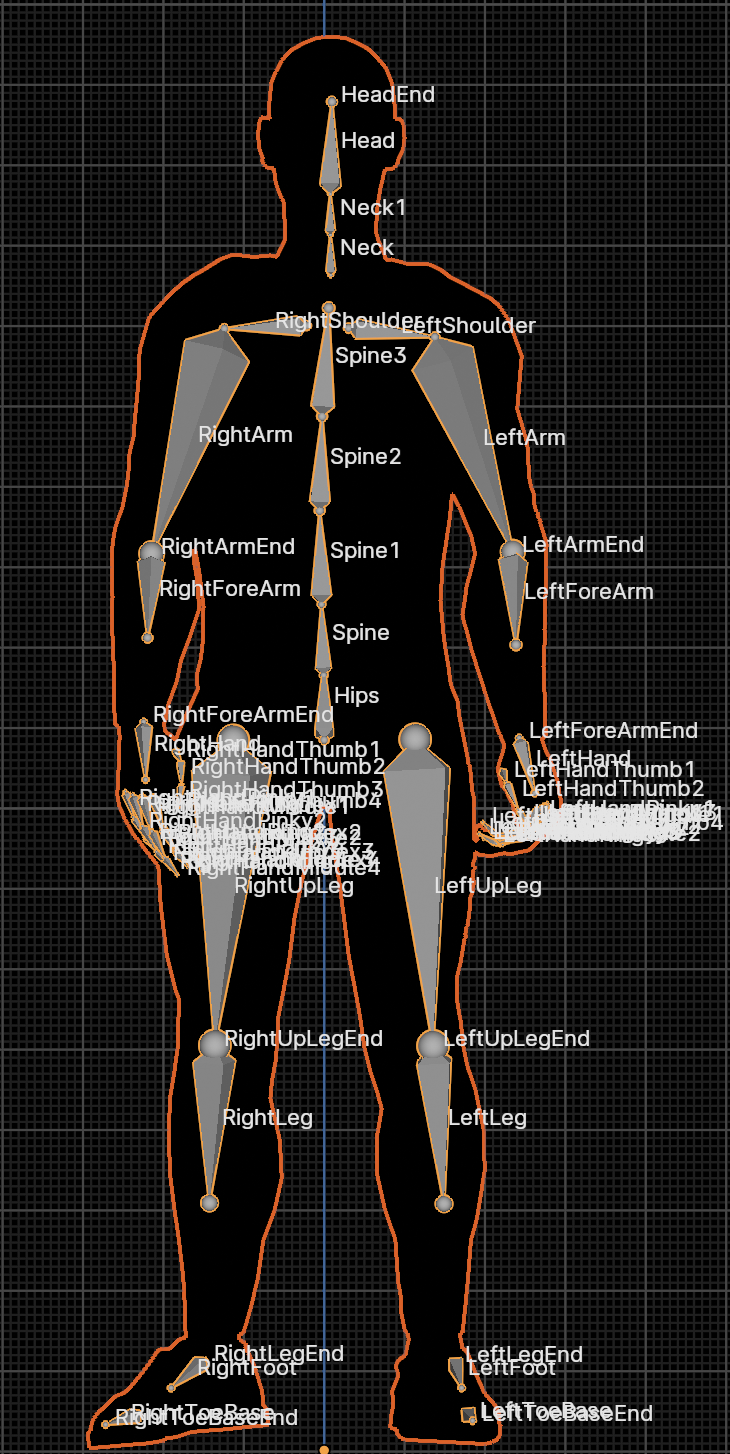
\includegraphics[height=10cm]{images/Skeleton.png}
		\caption{\small Khung xương và tên của các khớp của một khung xương trong mỗi khung hình.}
		\label{fig:Skeleton}
	\end{subfigure}
	\hfill
	\begin{subfigure}{0.49\textwidth}
		\centering
		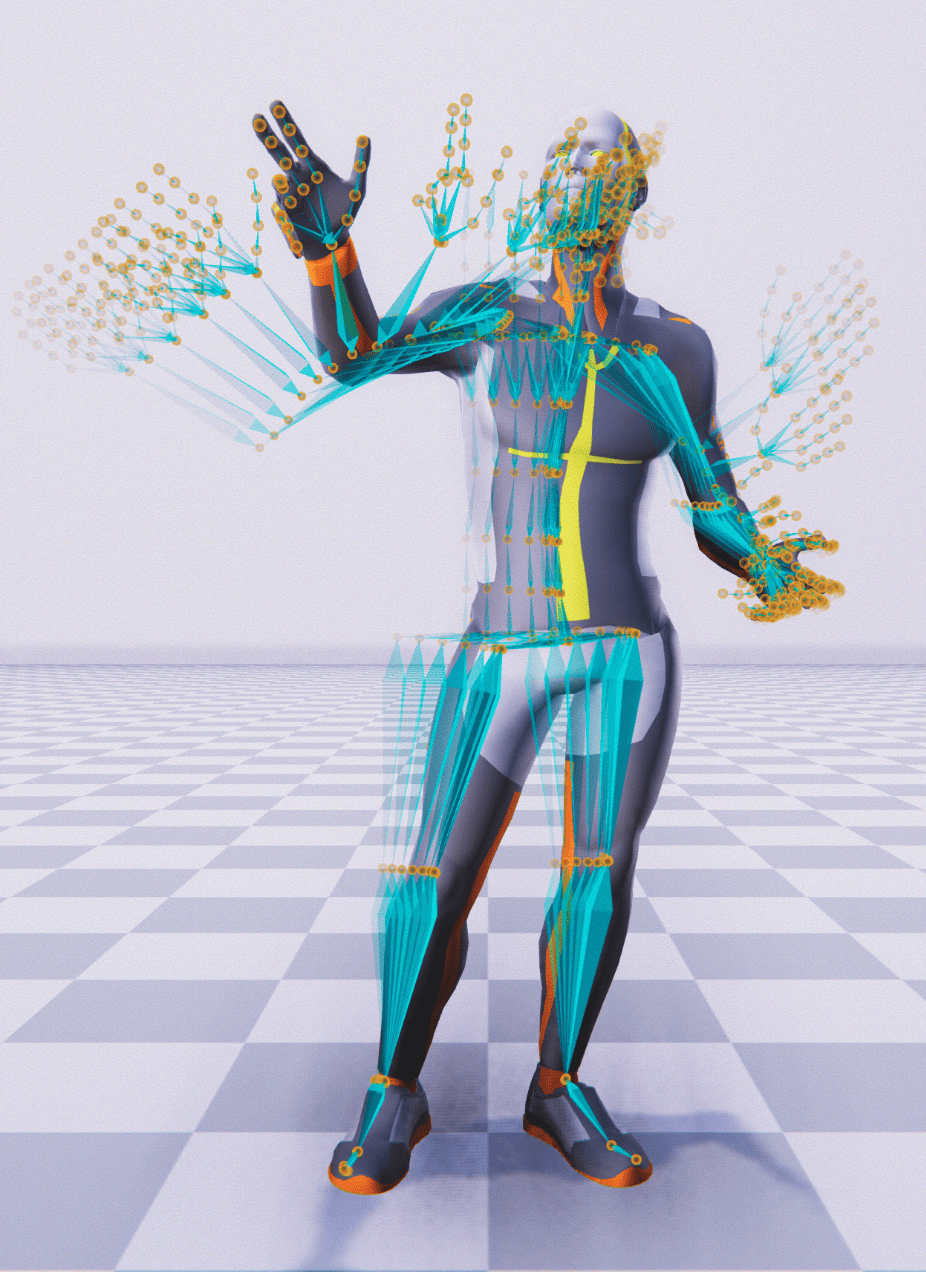
\includegraphics[height=10cm]{images/MotionPastAndFuture.png}
		\caption{\small Chuỗi chuyển động của cử chỉ bao gồm 6 cử chỉ quá khứ và 6 cử chỉ tương lai.}
		\label{fig:MotionPastAndFuture}
	\end{subfigure}
\end{figure}

Mỗi khung hình chuyển động của một nhân vật hay khung xương (skeleton) bao gồm dữ liệu về toạ độ vị trí và vận tốc theo thời gian.
Ở đây dữ liệu của chúng tôi của một khung xương với mỗi khung hình (frame) bao gồm:

\begin{equation} \label{eq:gesturevector}
\mathbf{g} = \Big[ \mathbf{p}_{\text{root}},  \mathbf{r}_{\text{root}},
\mathbf{ p }'_{\text{root}},  \mathbf{r}'_{\text{root}},
\mathbf{p}_{\text{joins}},  \mathbf{r}_{\text{joins}},
\mathbf{p}'_{\text{joins}},  \mathbf{r}'_{\text{joins}},
\mathbf{d}_{\text{gaze}}
\Big]
\end{equation}



Trong  đó với mỗi $\mathbf{g} \in \mathbb{R}^{1141}$ bao gồm:
{
\begin{itemize}
	\item $\mathbf{p}_{\text{root}} \in \mathbb{R}^3$: Toạ độ của điểm gốc
	\item $\mathbf{r}_{\text{root}} \in \mathbb{R}^4$: Góc quay của điểm gốc
	\item $\mathbf{p}'_{\text{root}} \in \mathbb{R}^3$: Vận tốc thay đổi của toạ độ gốc
	\item $\mathbf{r}'_{\text{root}} \in \mathbb{R}^3$: Vận tốc thay đổi của góc quay gốc
	
	\item $\mathbf{p}_{\text{joins}} \in \mathbb{R}^{3 n_{\text{join} }}$: Toạ độ của các khung xương
	\item $\mathbf{r}_{\text{joins}} \in \mathbb{R}^{6 n_{\text{join} }}$: Góc quay của các khung xương theo mặc phẳng X và Y
	\item $\mathbf{p}'_{\text{joins}} \in \mathbb{R}^{3n_{\text{join} }}$: Vận tốc thay đổi của toạ độ các khung xương
	\item $\mathbf{r}'_{\text{joins}} \in \mathbb{R}^{3n_{\text{join} }}$: Vận tốc thay đổi của góc quay các khung xương
	\item $\mathbf{d}_{\text{gaze}} \in \mathbb{R}^3$: Là hướng nhìn
\end{itemize}}


%\begin{figure}
%	\centering
%	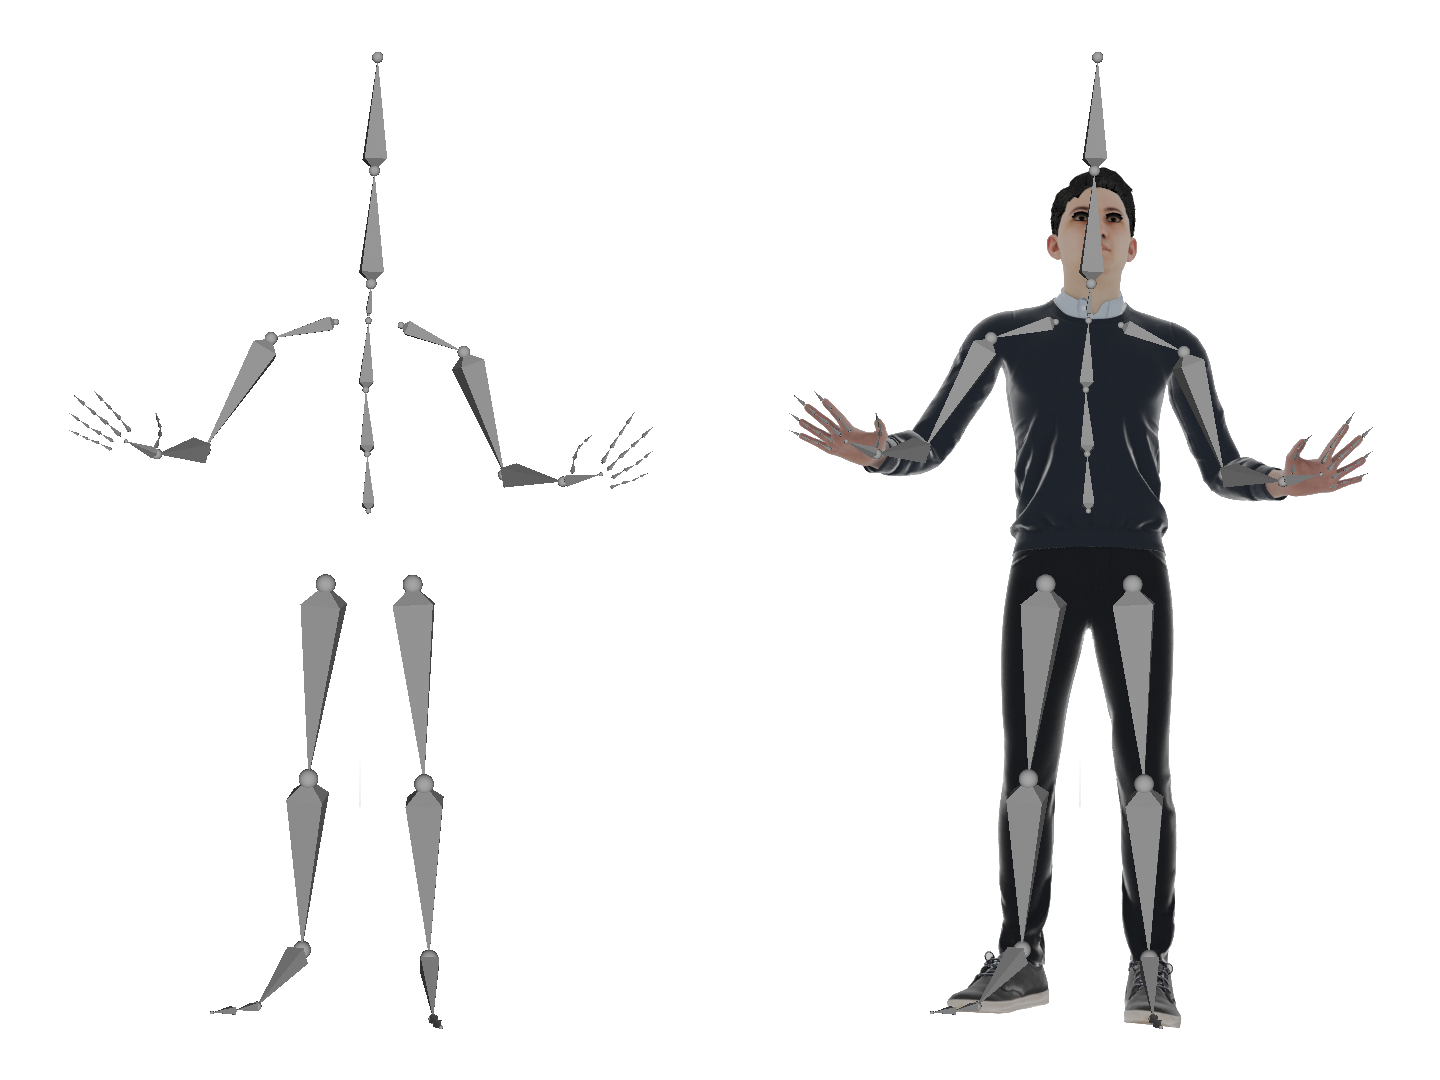
\includegraphics[width=0.8\linewidth]{images/skeleton_sample.png}
%	\caption{Minh họa một cử chỉ và mô hình nhân vật}
%	\label{fig:software}
%\end{figure}


Tổng cộng có $75$ khớp (joins) hay $n_{\text{join}} = 75$, với mỗi khung hình (frame) ta sẽ có một vector gồm 1141 chiều.
Tập dữ liệu là tập nhiều chuỗi cử chỉ với độ dài tuỳ ý, từ mỗi cử chỉ độ dài tuỳ tý ta sẽ cắt thành các đoạn $N + M$ khung hình, $g \in \mathbb{R}^{(N + M) \times 1141}$ , trong đó cử chỉ $\mathbf{s} \in \mathbb{R}^{N \times 1141}$ đầu tiên là cử chỉ khởi tạo (seed gesture), $\bx \in \mathbb{R}^{M \times 1141}$ cử chỉ tiếp theo cho việc dự đoán.


Dữ liệu âm thanh $\mathbf{a}_{\text{raw}} \in \mathbb{R}^{ \text{length } }$ là chuỗi âm thanh thô được đọc ở sample rate 16000, sau đó được cắt thành $\mathbf{a} \in \mathbb{R}^{64000}$ tương ứng với 4 giây.
% để  là một chuỗi waveform có độ dài tương ứng với cử chỉ được đọc với sample rate là 16000. 
%\setcounter{figure}{2}
\begin{figure}[H]
	\centering
	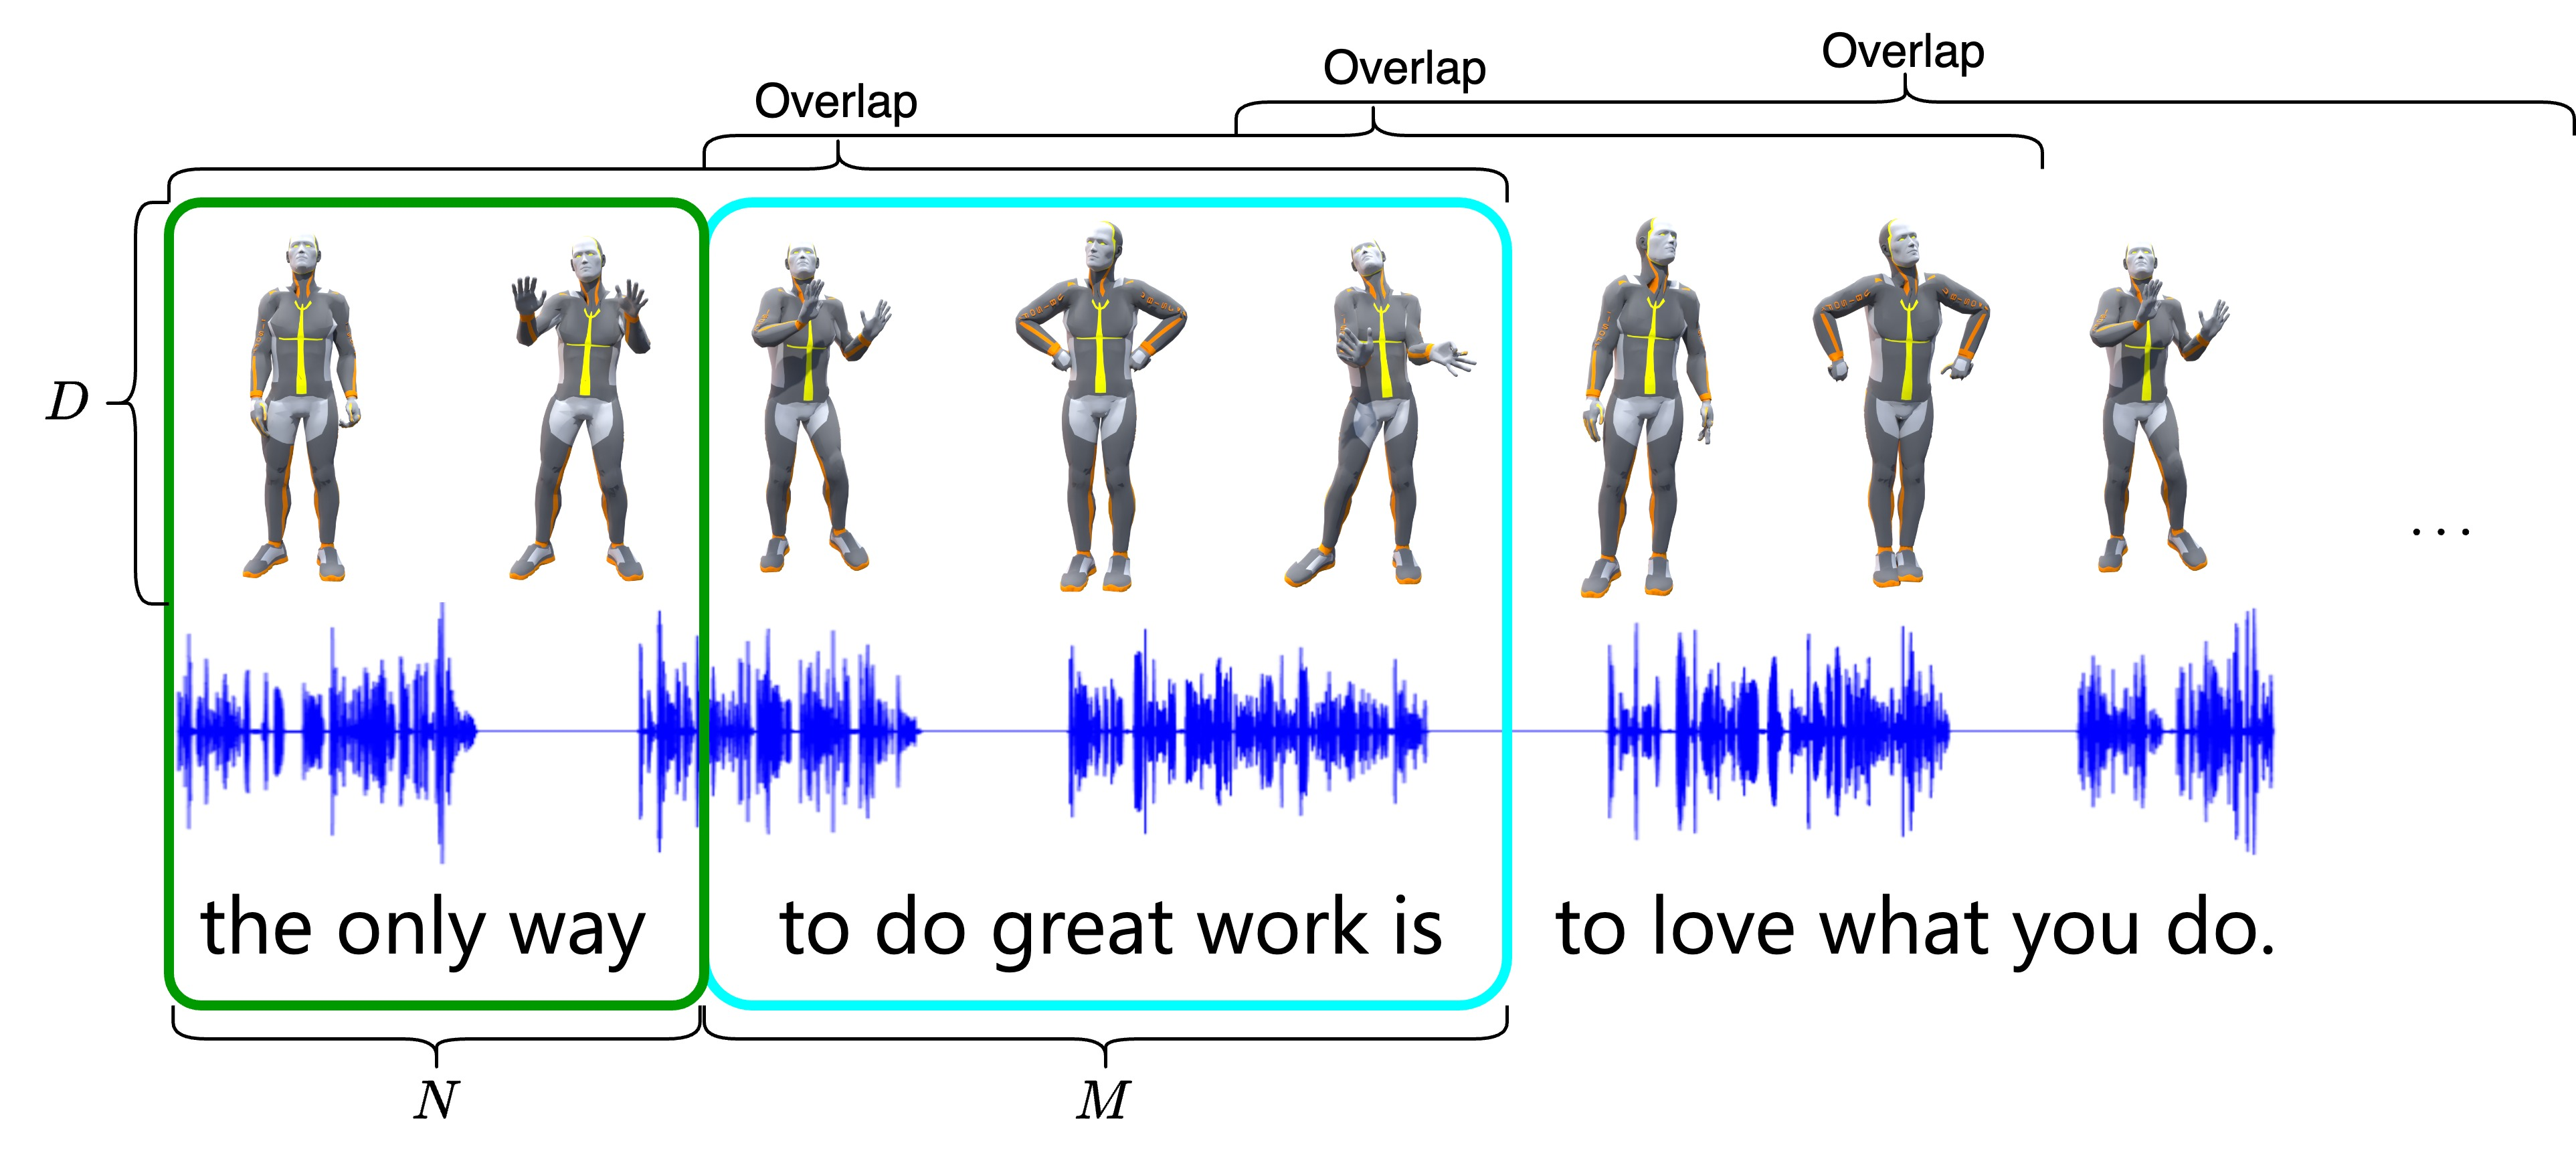
\includegraphics[width=\linewidth]{GestureSeries.jpg}
	\caption{Minh hoạ một chuỗi cử chỉ, ta lấy $N$ frame đầu làm cử chỉ khởi tạo $\mathbf{s}$ (seed gesture) và $M$ khung hình còn lại làm cử chỉ để học}
	\label{fig:GestureSeries}
\end{figure}


Quá trình xử lý dữ liệu được trình bày đầy đủ ở phụ lục \ref{Appendix2}.


%Quá trình chuyển từ không gian Eule sang không gian Quaternion được minh hoạ ở phụ lục \ref{}
%Chuỗi waveform sẽ được cắt thành các đoạn chồng nhau, áp dụng Hamming windows, và áp dụng thuật toán fast fourier transform để biến đổi chuỗi âm thanh thành các hệ số thể hiện cường độ của các tần số trong chuỗi âm thanh, các hệ số này được làm tròn thành các đoạn tần số (frequency bins), các đoạn hệ số này được chuẩn hoá theo hệ cơ số log để tương ứng với cảm nhận của tai người để có được đặc trưng MFCC $\mathbf{a} \in \mathbb{R}^{\text{size} \times \mathcal{C}}$ trong đó $\mathcal{C}=13$ là số frequency bins. 


% \begin{figure}
%     \centering
%     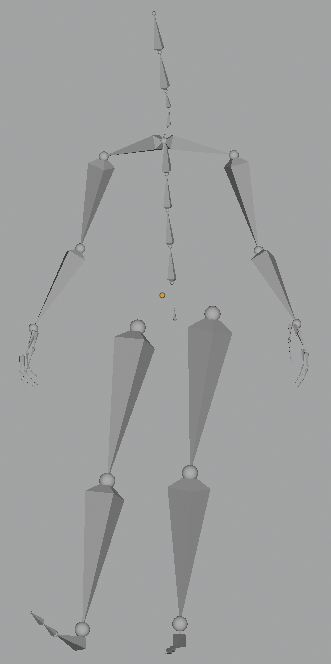
\includegraphics[width=3cm]{images/gesture_sample.png}
%     \caption{Minh họa cử chỉ}
%     \label{fig:gesture_sample}
% \end{figure}

\section{Các khó khăn cần giải quyết}

Có rất nhiều khó khăn trong việc xây dựng một mô hình có thể học được các đăng trưng cử chỉ hội thoại như con người 
%theo thời gian thực:

Thứ nhất, \textit{dữ liệu không đủ nhiều và chất lượng}, chi phí để tạo ra một bộ dữ liệu trong ngành công nghiệp Motion Capture có chất lượng và quy mô lớn để ứng dụng vào trong thực tế là rất lớn.

Thứ hai, \textit{sự thiếu đồng nhất của về ngữ cảnh của các loại dữ liệu}, các bộ dữ liệu về văn bản thường rất nhiều hơn so với giọng nói và cũng không thể biết được văn bản đó được tạo bởi người nào, sự đồng bộ giữa giọng nói và cảm xúc lúc nói cũng thiếu trong việc tạo tập dữ liệu. Ngoài ra, các dữ liệu văn bản lại được nói bởi rất nhiều người khác nhau và ở nhiều nội dung và chủ đề khác nhau.
 
Thứ ba, \textit{sự phân bố không cân xứng về  dữ liệu giữa các loại đăng trưng cần học}. Các dữ liệu dùng cho nghiên cứu cử chỉ hiện nay thường tập trung vào ngôn ngữ Tiếng Anh, các cử chỉ có sự phân bố không cân xứng giữa khi nói, khi hỏi, khi im lặng.

Thứ tư, \textit{chi phí tính toán với nhiều loại dữ liệu của mô hình rất lớn}. Với đầu vào của mô hình gồm rất nhiều loại dữ liệu khác nhau như văn bản, tiếng nói và điểm 3D, nên cần rất nhiều lớp encode cho từng loại dữ liệu cũng là rào cản không nhỏ bởi chi phí tính toán khi huấn luyện và khi suy luận. Nếu giảm thông tin dữ liệu đầu vào cũng sẽ giảm kết quả suy luận của mô hình khi sinh cử chỉ.

Cuối cùng, \textit{các bước xử lý phải yêu cầu tuần tự}, cách hiệu quả nhất để con người tương tác với máy tính là thông qua giọng nói và nhập từ bàn phím, tuy nhiên việc xử lý được văn bản và giọng nói để làm đầu vào cho mô hình phải thực hiện tuần tự, độ trễ để có thể suy luận trong sản phẩm thực tế cũng là một vấn đề bởi người dùng không thể đợi lâu để nhận được kết quả cử chỉ và từ cử chỉ đó biểu diễn lên máy tính bằng kỹ thuật đồ họa máy tính.


\section{Đóng góp dự kiến}

\begin{itemize}
	\item Dựa trên tập dữ liệu có sẵn, chúng tôi chuyển âm thanh của dữ liệu thành văn bản, và dùng văn bản đó để làm dữ liệu huấn luyện mới.
%	\item Tích hợp đặc trưng văn bản vào mô hình DiffuseStyleGesture:** Chúng tôi cải tiến DiffuseStyleGesture bằng cách đưa thông tin văn bản vào quá trình khử nhiễu có điều kiện, giúp hệ thống sinh ra các cử chỉ chi tiết và phù hợp hơn với nội dung hội thoại.
	
	
	\item Dựa trên mô hình cơ bản DiffuseStyleGesture, chúng tôi mở rộng thêm đặc trưng văn bản trong quá trình khử nhiễu có điều kiện.
	
	\item Chúng tôi sử dụng Unity để render, trích xuất dữ liệu và trực quan hoá kết quả sinh cử chỉ.
	
	\item Chúng tôi xây dựng hệ thống kết xuất, và minh hoạ chương trình bằng Unity
	
	
	
%	với thông tin thời gian cho việc sinh cử chỉ kèm theo lời nói dựa trên âm thanh. Nhờ mô hình diffusion, chúng tôi có thể kiểm soát một cách linh hoạt cử chỉ được sinh ra, ví dụ: chỉnh sửa phong cách của cử chỉ, thiết lập cử chỉ khởi tạo, và sinh cử chỉ đa dạng.
	
%	\item Chúng tôi sử dụng cross-local attention và self-attention để để học được bối cảnh và những quan hệ giữa cử chỉ và lời nói.
%	
%	\item Các thử nghiệm mở rộng chỉ ra rằng mô hình của chúng tôi có thể sinh ra cử chỉ giống người, phù hợp với lời nói (speech-appropriateness), phù hợp với cảm xúc (style-appropriateness) vượt trội so với các phương pháp sinh cử chỉ hiện có.
\end{itemize}



%\item **Sử dụng Unity để render, trích xuất dữ liệu và trực quan hoá kết quả sinh cử chỉ:** Chúng tôi triển khai Unity như một công cụ trực quan hóa để mô phỏng và hiển thị kết quả của hệ thống sinh cử chỉ. Với các tính năng mô phỏng 3D mạnh mẽ, Unity cho phép chúng tôi kiểm nghiệm và đánh giá hiệu quả của các cử chỉ được sinh ra từ mô hình, đồng thời hỗ trợ trực quan hóa các đặc trưng chuyển động của cử chỉ. Hệ thống cũng sẽ được phát triển để cho phép dễ dàng trích xuất dữ liệu cử chỉ và so sánh kết quả trực quan giữa các mô hình khác nhau, giúp nâng cao tính khả thi và giá trị thực nghiệm của hệ thống.
%
%\item **Xây dựng hệ thống kết xuất và minh hoạ chương trình bằng Unity:** Ngoài việc render và trực quan hóa kết quả sinh cử chỉ, chúng tôi phát triển hệ thống kết xuất hoàn chỉnh, bao gồm các thành phần giúp dễ dàng minh hoạ quá trình sinh cử chỉ theo từng giai đoạn. Hệ thống này không chỉ cung cấp công cụ để kiểm nghiệm chất lượng cử chỉ sinh mà còn giúp mô tả rõ ràng từng bước trong quá trình sinh cử chỉ, từ giai đoạn tiền xử lý dữ liệu, khử nhiễu, đến việc ứng dụng các đặc trưng văn bản và âm thanh để tạo ra cử chỉ. Điều này sẽ làm tăng tính minh bạch và khả năng giải thích của hệ thống, đồng thời hỗ trợ các nhà nghiên cứu và người dùng dễ dàng quan sát và hiểu sâu hơn về các bước sinh cử chỉ. 

%\begin{itemize}
%\item Chúng tôi mở rộng mô hình diffusion với thông tin thời gian cho việc sinh cử chỉ kèm theo lời nói dựa trên âm thanh. Nhờ mô hình diffusion, chúng tôi có thể kiểm soát một cách linh hoạt cử chỉ được sinh ra, ví dụ: chỉnh sửa phong cách của cử chỉ, thiết lập cử chỉ khởi tạo, và sinh cử chỉ đa dạng.
%
%\item Chúng tôi sử dụng cross-local attention và self-attention để để học được bối cảnh và những quan hệ giữa cử chỉ và lời nói.
%
%\item Các thử nghiệm mở rộng chỉ ra rằng mô hình của chúng tôi có thể sinh ra cử chỉ giống người, phù hợp với lời nói (speech-appropriateness), phù hợp với cảm xúc (style-appropriateness) vượt trội so với các phương pháp sinh cử chỉ hiện có.
%\end{itemize}


% Đầu vào của hệ thống trí tuệ nhân tạo cho việc sinh cử chỉ bao gồm: 

% Tức đã có input (audio/text) sang output (text). Nhưng chưa có từ text sang 1 visual.

% Để xây dựng 1 virtual human assitant mà tương tác được cần sinh ra Output:

% - Hình ảnh: text to visual: 3D scan da người, các texture, mesh và quan trọng nhất là cử chỉ của người đó.

% - Âm thanh: text to speech.

% Để học được các cử chỉ thì dữ liệu đầu vào dĩ nhiên bao gồm các keypoint 3D về cử chỉ, dữ liệu cử chỉ bao gồm cử chỉ của cơ thể ($\Omega_{\text{Body}}$) cử chỉ của bàn tay ($\Omega_{\text{Hand}}$) và biểu cảm khuôn mặt ($\Omega_{\text{Facial}}$).

% $$
% \Omega = \{ \Omega_{\text{Speaker_ID}}; \Omega_{\text{Emotion_ID}}; \Omega_{\text{Text}}; \Omega_{\text{Speech}}; \\
% \Omega_{\text{Facial}}; \Omega_{\text{Hand}}; \Omega_{\text{Body}}
% \} 
% $$

% \section{Bài toán sinh cử chỉ}

%Đầu vào của mô hình sinh cử chỉ là chuỗi văn bản (text), chuỗi lời nói (speech) và tọa độ cử chỉ khởi tạo, với đầu ra là chuỗi cử chỉ được sinh ra tương ứng với văn bản và lời nói tương ứng.

%là các keypoint chuyển động trên không gian tọa độ 3 chiều của cử chỉ cơ thể (\textbf{body gesture}), cử chỉ bàn tay (\textbf{hand gesture}) và biểu cảm khuôn mặt (\textbf{facial expression}), tương ứng từng cử chỉ là văn bản (\textbf{text}) và giọng nói (\textbf{speech}). Mỗi người đều có phong cách cử chỉ khác nhau và cảm xúc lúc nói khác nhau nên cũng cần phải có thêm thông tin về người nói (\textbf{speaker identity}) và cảm xúc lúc nói (\textbf{emotions}) tương ứng. 
%
%Kết quả đầu ra của việc sinh cử chỉ là chuỗi các cử chỉ (gesture), với mỗi cử chỉ là tập các điểm trong tọa độ 3D ( bao gồm vị trí ($x, y, z$) và góc quay ($r_{x}, r_{y}, r_{z}$ ) ) như hình minh họa 




% Ngôn ngữ để viết và trình bày báo cáo khóa luận tốt nghiệp, đồ án tốt nghiệp, thực tập tốt nghiệp (sau đây gọi chung là báo cáo) là tiếng Việt hoặc tiếng Anh. 
% Trường hợp chọn ngôn ngữ tiếng Anh để viết và trình bày báo cáo,  sinh viên cần có đơn đề nghị, được cán bộ hướng dẫn (CBHD) đồng ý và nộp cho bộ phận Giáo vụ của Khoa vào thời điểm đăng ký đề tài để xin ý kiến.
% Báo cáo viết và trình bày bằng tiếng Anh phải có bản tóm tắt viết bằng tiếng Việt.


%Tóm tắt luận văn được trình bày nhiều nhất trong 24 trang in trên hai mặt giấy, cỡ chữ Times New Roman 11 của hệ soạn thảo Winword hoặc phần mềm soạn thảo Latex đối với các chuyên ngành thuộc ngành Toán.

%Mật độ chữ bình thường, không được nén hoặc kéo dãn khoảng cách giữa các chữ.
%Chế độ dãn dòng là Exactly 17pt.
%Lề trên, lề dưới, lề trái, lề phải đều là 1.5 cm.
%Các bảng biểu trình bày theo chiều ngang khổ giấy thì đầu bảng là lề trái của trang.
%Tóm tắt luận án phải phản ảnh trung thực kết cấu, bố cục và nội dung của luận án, phải ghi đầy đủ toàn văn kết luận của luận án.
%Mẫu trình bày trang bìa của tóm tắt luận văn (phụ lục 1).

\chapter{CÁC CÔNG TRÌNH LIÊN QUAN}
\label{Chapter2}

Bài toán sinh cử chỉ là cũng tương tự như các bài toán khác đều đã nghiên cứu và phát triển song hành cùng các phương pháp học máy truyền thống cũng như các phương pháp học sâu hiện đại ngày nay, gồm các nhóm phương pháp dựa trên luật và các phương pháp dựa trên dữ liệu. 

\section{Mối quan hệ giữa cử chỉ và lời nói}

Cử chỉ được chia thành 6 nhóm chính theo ngôn ngữ  học \cite{ekman1969repertoire}, \cite{sebeok2011advances} cử chỉ thích nghi (adaptors), cử chỉ biểu tượng (emblems), cử chỉ chỉ định (deictics), cử chỉ biểu trưng (iconics), cử chỉ ẩn dụ (metaphorics) và cử chỉ nhấn mạnh (beat).

 Trong đó, cử chỉ nhấn mạnh không liên quan trực tiếp đến ngữ nghĩa lời nói \cite{kipp2005gesture} nhưng rất quan trọng để tạo sự hài hòa về nhịp điệu giữa lời nói và cử chỉ  \cite{sebeok2011advances} . Tuy nhiên, lời nói và cử chỉ nhấn mạnh không đồng bộ hoàn toàn về mặt nhịp điệu \cite{mcclave1994gestural}, nên việc học mối liên hệ thời gian giữa chúng gặp khó khăn \cite{bhattacharya2021speech2affectivegestures}, \cite{kucherenko2020gesticulator}, \cite{yoon2020speech}.

Cử chỉ liên quan đến các cấp độ khác nhau của thông tin lời nói \cite{sebeok2011advances}. Ví dụ, cử chỉ biểu tượng như cầm ngược cái ngón cái thường đi kèm với ngữ nghĩa cấp cao như tốt hay tuyệt vời, trong khi cử chỉ nhấn mạnh thường xuất hiện cùng với sự nhấn mạnh âm thanh cấp thấp. Nhiều nghiên cứu trước đây chỉ sử dụng các đặc trưng được trích xuất từ lớp cuối cùng của bộ mã hóa âm thanh để tổng hợp cử chỉ \cite{alexanderson2020style},  \cite{bhattacharya2021speech2affectivegestures}, \cite{kucherenko2021large}, \cite{qian2021speech},  \cite{yoon2022genea}. Tuy nhiên, cách thiết lập này có thể khuyến khích bộ mã hóa trộn lẫn thông tin lời nói ở nhiều cấp độ khác nhau vào cùng một đặc trưng, gây ra sự mơ hồ và tăng độ khó khăn trong việc khai thác các dấu hiệu nhịp điệu và ngữ nghĩa rõ ràng.

%Trong bài báo này, chúng tôi tập trung vào việc tạo ra cử chỉ trên đi kèm lời nói có thể đồng hành với một loạt các nội dung lời nói rộng - từ một câu đến bài phát biểu công khai, nhằm đạt được kết quả thuyết phục cả về nhịp điệu và ngữ nghĩa. Quan sát đầu tiên của chúng tôi là cử chỉ có thể được coi là một dạng nhảy đặc biệt dưới nhịp điệu thay đổi. Chúng tôi phát triển một khuôn khổ chuẩn hóa và tạo ra nhịp điệu để đối phó với thách thức tạo ra cử chỉ đồng bộ với lời nói, phân đoạn lời nói thành các đoạn ngắn tại các nhịp âm thanh, chuẩn hóa các đoạn này thành các khối chuẩn có cùng độ dài, tạo ra cử chỉ cho mỗi khối và căn chỉnh chuyển động được tạo ra với nhịp điệu của lời nói. Khuôn khổ này, được lấy cảm hứng một phần từ các nghiên cứu gần đây về tạo múa \cite{aristidou2022rhythm}, cung cấp cho mô hình cử chỉ một gợi ý rõ ràng về nhịp điệu, cho phép mô hình học hiệu quả mẫu cử chỉ nhấn mạnh trong một khối nhịp điệu. 
%Cả đánh giá định lượng với một chỉ số nhịp điệu mới và đánh giá chất lượng với nghiên cứu người dùng đều cho thấy cử chỉ được tạo ra bởi quy trình này thể hiện sự đồng bộ tự nhiên với lời nói.

Như được chỉ ra trong các tài liệu ngôn ngữ học \cite{kipp2005gesture} \cite{neff2008gesture} \cite{webb1997linguistic},
cử chỉ được sử dụng trong cuộc hội thoại hàng ngày có thể được chia thành một số lượng hạn chế các đơn vị ngữ nghĩa với các biến thể chuyển động khác nhau. Chúng tôi giả định rằng các đơn vị ngữ nghĩa này, thường được gọi là từ ngữ, liên quan đến các đặc trưng cấp cao của âm thanh lời nói, trong khi các biến thể chuyển động được xác định bởi các đặc trưng âm thanh cấp thấp. Do đó, chúng tôi tách rời các đặc trưng cấp cao và cấp thấp từ các lớp khác nhau của bộ mã hóa âm thanh và học các ánh xạ giữa chúng và các từ ngữ cử chỉ và các biến thể chuyển động, tương ứng. Các thử nghiệm chứng minh cơ chế này thành công trong việc tách rời các đặc trưng ở nhiều cấp độ của cả lời nói và chuyển động và tổng hợp các cử chỉ phù hợp về mặt ngữ nghĩa và có phong cách.

\section{Tổng quan các phương pháp cho bài toán sinh cử chỉ}

\subsection{Phương pháp dựa trên luật}

Các phương pháp dựa trên luật thường ánh xạ (mappings) từng âm thanh với từng đơn vị cử chỉ \cite{huang2012robot}. Và luật được tạo thủ công. Phương pháp dựa trên luật thì chúng ta có thể dễ dàng điều khiển kết quả của mô hình và có khả năng giải thích tốt kết quả dự đoán của mô hình.
Tuy nhiên chi phí để tạo thủ công là không khả thi để xây dựng cho các ứng dụng phức tạp đòi hỏi phải xử lý một lượng dữ liệu rất lớn.

\subsection{Phương pháp dựa trên thống kê}

Tương tự như phương pháp dựa trên luật, phương pháp dựa trên dữ liệu cũng ánh xạ các đặc trưng của âm thanh tương ứng với cử chỉ nhưng thay vì làm thủ công thì được sử dụng học một cách tự động dựa trên dữ liệu.
Trong đó có hai phương pháp chính là phương pháp thống kê và phương pháp dựa trên dữ liệu.

%\subsubsection{Phương pháp thống kê}

Phương pháp thống kê sử dụng phân phối xác xuất để tìm sự tương đồng giữa các đặc trưng âm thanh và cử chỉ \cite{levine2010gesture}. Tác giả \cite{neff2008gesture} xây dựng mô hình để học từng phong cách của từng người nói.

\subsection{Phương pháp học sâu}

\setcounter{figure}{3}
\begin{figure}[H]
	\centering
	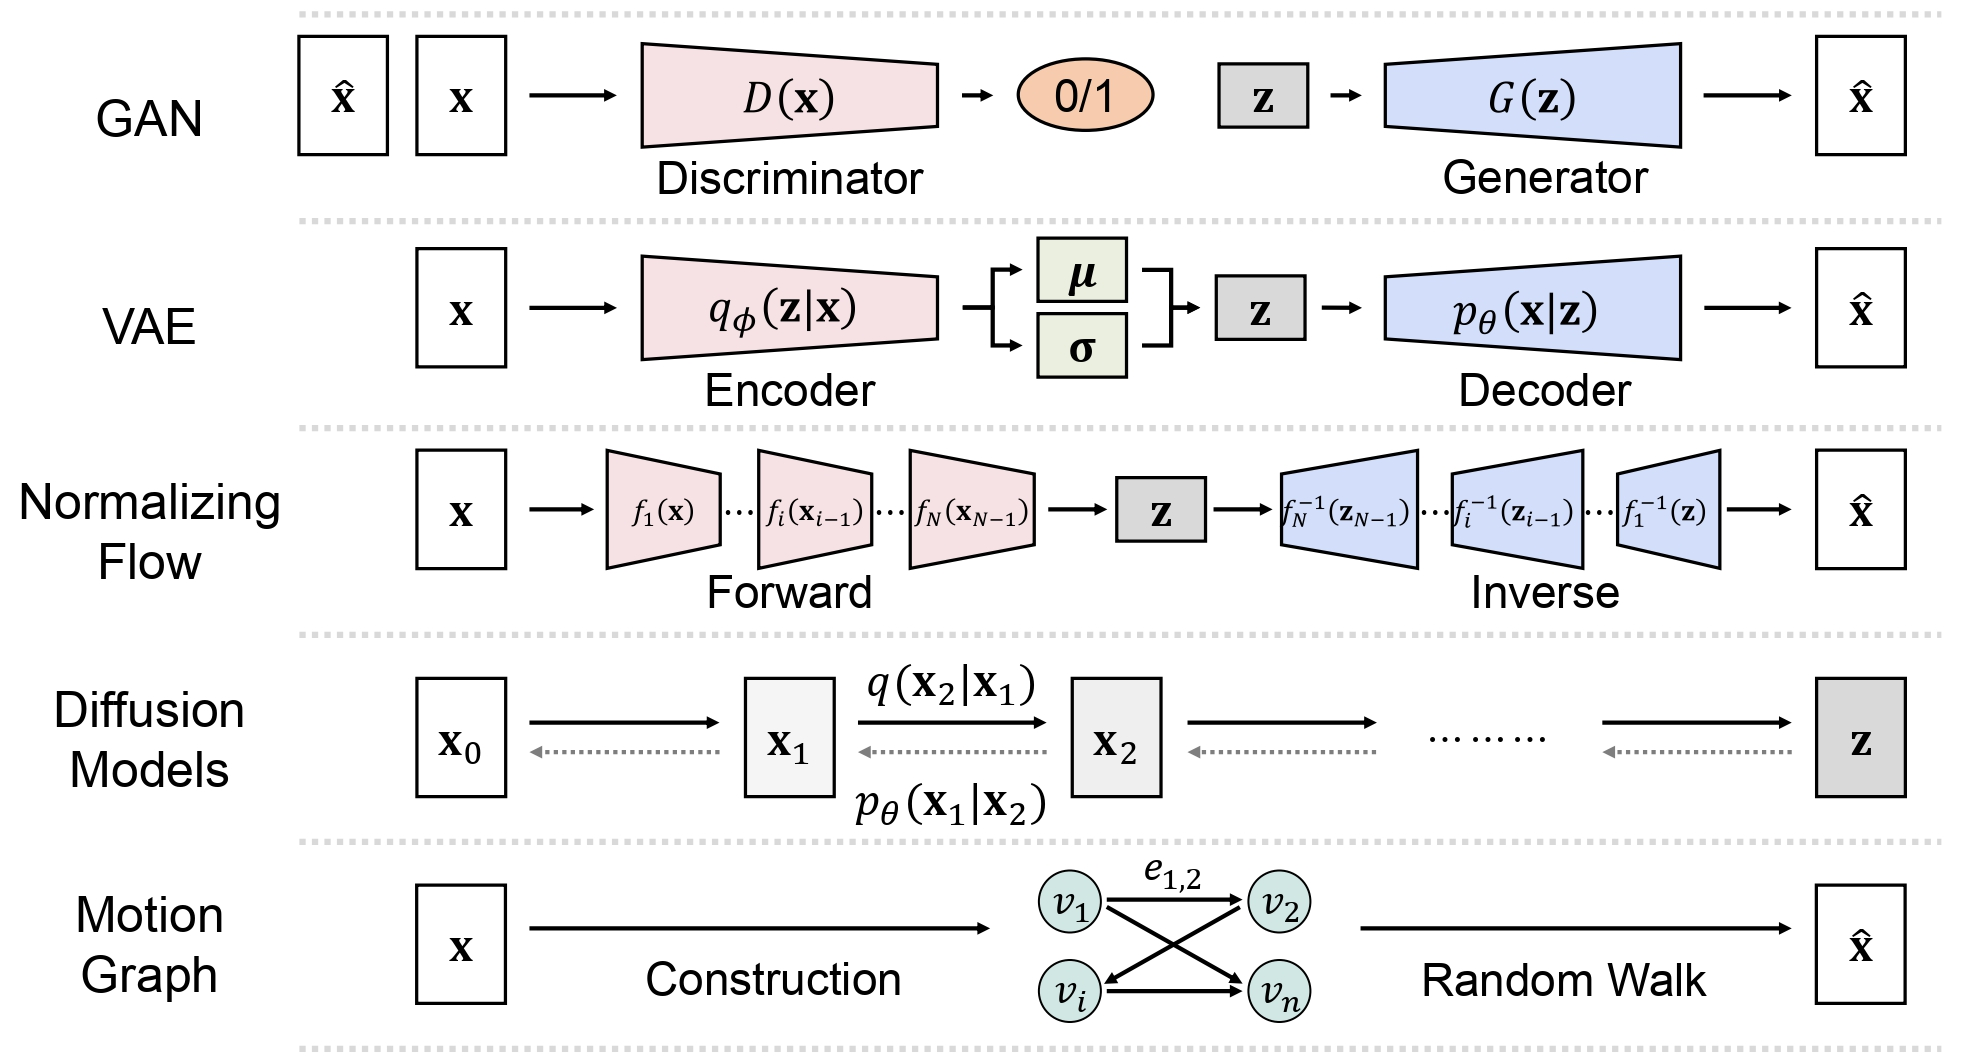
\includegraphics[width=0.8\textwidth]{Survey.jpg}
	\caption{Tổng quan về các mô hình tạo sinh khác nhau.}
	\label{fig:generative-models}
\end{figure}

Phương pháp sinh cử chỉ được chia thành hai nhóm chính. Bao gồm các mô hình ước lượng log likelihood (likelihood-base model)  và phương pháp dựa vào các mô hình sinh ngầm định (implicit generative models).

\subsubsection{Likelihood-base Model}

Phương pháp học ước lượng log likelihood là phương pháp học trực tiếp từ hàm mật độ xác xuất (probability density) thông qua maximum likelihood. Các phương pháp điển hình là autoregressive models, normalizing flow models, energy-based models (EBMs)
, và variational auto-encoders (VAEs).

%Phương pháp học sâu sử dụng mạng nơ-ron (neural) thông qua nhiều lớp ẩn để học một cách tự động các phối xác xuất giữa cử chỉ và âm thanh.

Mô hình được kết hợp với văn bản đầu vào được gắn thẻ với chủ đề, trọng tâm câu và thành ngữ để tạo ra các kịch bản cử chỉ, sau đó được ánh xạ sang một chuỗi các cử chỉ được chọn từ một từ điển hoạt họa. \cite{chiu2015predicting} huấn luyện một model classifier neuron network để chọn một đơn vị cử chỉ phù hợp dựa trên đầu vào là lời nói. 
%Nghiên cứu gần đây đã bắt đầu tận dụng học sâu và huấn luyện các mô hình kết thúc đến cuối sử dụng dữ liệu cử chỉ thô trực tiếp, giải phóng các nỗ lực thủ công trong thiết kế từ điển cử chỉ và các quy tắc ánh xạ.

Cử chỉ có thể được tổng hợp bằng các mô hình xác định như perceptron đa tầng (MLP) \cite{kucherenko2020gesticulator}, recurrent neural networks \cite{bhattacharya2021speech2affectivegestures}, \cite{liu2022learning}, \cite{hasegawa2018evaluation}, \cite{yoon2020speech}, convolutional networks \cite{habibie2021learning} và transformer \cite{bhattacharya2021text2gestures} 

%và các mô hình như normalizing flow \cite{alexanderson2020style}, 
%phương pháp học code  \cite{xu2022freeform}.

\subsubsection{Implicit Generative Models}

Trong các phương pháp dựa vào mô hình sinh ngầm định, phân phối của dữ liệu được học một cách ngầm định thông qua việc quá sinh lấy mẫu (sampling). Ví dụ tiêu biểu nhất là mô hình generative adversarial networks (GANs). Khi dữ liệu được tổng hợp bằng cách chuyển phân phối dữ liệu ban đầu ở dạng phân phối chuẩn về phân phối của dữ liệu.

Trong mục tiêu theo chúng tôi sẽ trình bày các phương pháp sử dụng mô hình Diffusion.

%chuyển phân phối của dữ liệu ở dạng phân phối chuẩn hay ở một vị trí bất kỳ về phân phối chuẩn bằng hàm neuron network. 


%WGAN \cite{wu2021probabilistic}.



%\textbf{Bảng so sánh các phương pháp}
%
%\begin{table}[ht]
%	\centering
%	\begin{tabular}{|l|l|l|l|l|l|}
%		\hline
%		\textbf{Phương pháp} & \textbf{Loại mô hình} & \textbf{Đặc điểm nổi bật} & \textbf{Ưu điểm} & \textbf{Hạn chế} & \textbf{Tài liệu tham khảo} \\ \hline
%		VAE  & Autoencoder & Biểu diễn dữ liệu trong không gian tiềm ẩn & Tạo đặc trưng ẩn & Khó kiểm soát đầu ra & \cite{kingma2013auto} \\ \hline
%		VQ-VAE & Autoencoder (cải tiến) & Dùng codebook cho không gian tiềm ẩn & Biểu diễn chi tiết hơn & Phức tạp hơn & \cite{van2017neural} \\ \hline
%		RNN & Mạng hồi tiếp & Xử lý chuỗi dữ liệu & Tốt cho dữ liệu tuần tự & Khó huấn luyện & \cite{bhattacharya2021speech2affectivegestures} \\ \hline
%		Transformer & Mạng chú ý & Tạo cử chỉ qua cơ chế chú ý & Hiệu quả với dữ liệu dài & Yêu cầu nhiều tài nguyên & \cite{bhattacharya2021text2gestures} \\ \hline
%		WGAN & GAN & Học phân phối dữ liệu đối kháng & Tạo sự đa dạng & Khó huấn luyện & \cite{wu2021probabilistic} \\ \hline
%		Normalizing Flow & Mô hình xác suất & Học phân phối phức tạp & Hữu ích với dữ liệu phức tạp & Cần tài nguyên tính toán lớn & \cite{alexanderson2020style} \\ \hline
%		Diffusion Models & Mô hình sinh dữ liệu & Chi tiết cao, xử lý dữ liệu thiếu & Tạo cử chỉ chi tiết & Thời gian huấn luyện lâu & \cite{xu2022freeform} \\ \hline
%	\end{tabular}
%	\caption{So sánh các phương pháp sinh cử chỉ}
%\end{table}

%
%
%

\section{Giải pháp đề xuất}

\textit{Chương 3 của luận văn tập trung vào việc đề xuất giải pháp thay thế hệ thống quản lý cơ sở dữ liệu hiện tại là MSSQL bằng Greenplum. Đầu tiên, chương này trình bày các bước cần thiết để chuyển đổi từ MSSQL sang cơ sở dữ liệu phân tán, bao gồm phân tích các yêu cầu, lựa chọn công cụ hỗ trợ, và các thách thức có thể gặp phải trong quá trình chuyển đổi.}

\textit{Tiếp theo, chương này đi sâu vào quá trình lựa chọn Greenplum như là giải pháp thay thế cho MSSQL. Các tiêu chí lựa chọn bao gồm khả năng mở rộng, tính tương thích với hệ thống hiện tại, và khả năng xử lý dữ liệu lớn. Chương này cũng phân tích lý do tại sao Greenplum, với kiến trúc MPP (Massively Parallel Processing), lại phù hợp với yêu cầu của hệ thống ASP.NET Membership, đặc biệt là trong việc xử lý các tác vụ liên quan đến dữ liệu lớn và tối ưu hóa hiệu suất truy vấn.}

\textit{Cuối cùng, chương 3 đề cập đến quá trình chuẩn bị và triển khai Greenplum trong môi trường thử nghiệm, bao gồm việc cài đặt, cấu hình, và tích hợp với hệ thống hiện tại. Chương này cũng nhấn mạnh các kết quả ban đầu và những lợi ích mà Greenplum mang lại, như tăng cường hiệu suất xử lý và giảm thiểu thời gian truy vấn, từ đó giúp hệ thống đáp ứng tốt hơn các yêu cầu về khả năng mở rộng và hiệu suất.}

Trong thời đại kỹ thuật số hiện nay, việc quản lý và xử lý hiệu quả lượng dữ liệu ngày càng tăng trong các hệ thống thông tin là cực kỳ quan trọng. Các hệ thống cơ sở dữ liệu truyền thống như MSSQL đã chứng minh được nhiều giá trị, nhưng cũng bộc lộ những hạn chế nghiêm trọng trong việc đáp ứng nhu cầu về hiệu suất cao và khả năng mở rộng trong quản lý dữ liệu lớn. Như đã phân tích trong chương \ref{sec:introduction}, các vấn đề như tốc độ truy vấn chậm, quản lý tài nguyên không hiệu quả, và hạn chế về khả năng mở đã làm suy giảm hiệu suất của các hệ thống quản lý thành viên trực tuyến như ASP.NET Membership database. Để giải quyết những vấn đề này sẽ đề xuất việc chuyển đổi cơ sở dữ liệu ASP.NET Membership từ MSSQL sang một hệ thống cơ sở dữ liệu phân tán.

\subsection{Chuyển đổi MSSQL sang cơ sở dữ liệu phân tán}

Việc chuyển đổi cơ sở dữ liệu ASP.NET Membership từ một hệ thống cơ sở dữ liệu tập trung như MSSQL sang một hệ thống cơ sở dữ liệu phân tán đòi hỏi phải thực hiện một loạt các bước kỹ thuật chi tiết. Quá trình này không chỉ bao gồm việc di chuyển dữ liệu mà còn phải đảm bảo rằng tất cả các chức năng và hiệu suất của hệ thống được duy trì hoặc cải thiện. Dưới đây là các bước chi tiết để thiết lập hệ thống cơ sở dữ liệu phân tán phù hợp cho ASP.NET Membership Database.

\subsubsection{Kiến trúc lược đồ cơ sở dữ liệu}

\begin{figure}
    \centering
    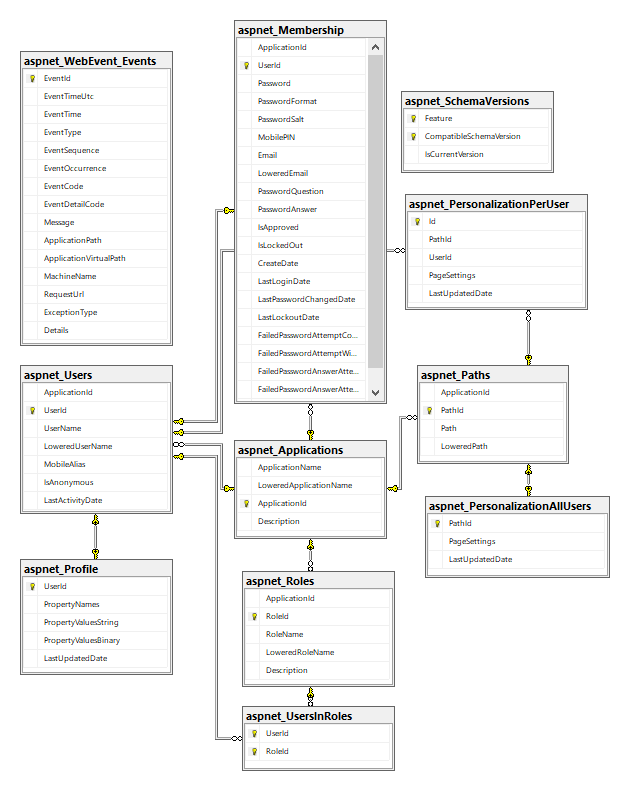
\includegraphics[width=1\linewidth]{schema.png}
    \caption{Sơ đồ ASP.NET Membership}
    \label{fig:schema}
\end{figure}

Cơ sở dữ liệu của hệ thống được thiết kế với cấu trúc phức tạp và logic, bao gồm nhiều bảng dữ liệu và mối quan hệ chặt chẽ giữa chúng. Hình ảnh \ref{fig:schema} minh họa rõ ràng cách các bảng dữ liệu chính liên kết với nhau, tạo nên một hệ thống cơ sở dữ liệu mạnh mẽ để hỗ trợ các chức năng cốt lõi của ứng dụng.

Bảng aspnet\_Users là trung tâm lưu trữ thông tin cơ bản về thành viên. Trong đó, cột UserId đóng vai trò là khóa chính, giúp định danh duy nhất từng thành viên. Các trường như UserName, MobileAlias, và LastActivityDate lưu trữ thông tin nhận diện và hoạt động của thành viên, hỗ trợ việc theo dõi và quản lý tài khoản.

Liên kết chặt chẽ với bảng này là aspnet\_Membership, nơi lưu trữ các thông tin liên quan đến bảo mật và trạng thái tài khoản thành viên. UserId trong bảng aspnet\_Membership là khóa ngoại, liên kết với aspnet\_Users, tạo ra mối quan hệ 1-1 giữa thông tin thành viên và thông tin thành viên. Các trường như Password, PasswordSalt, IsApproved, và LastLoginDate giúp quản lý quá trình xác thực và bảo mật tài khoản, đảm bảo rằng chỉ những thành viên hợp lệ mới có thể truy cập vào hệ thống.

aspnet\_Roles là bảng quản lý vai trò trong hệ thống. Mỗi vai trò được định danh bởi RoleId, và bảng này kết nối với aspnet\_Users thông qua bảng nối aspnet\_UsersInRoles. Bảng nối này sử dụng các khóa ngoại UserId và RoleId để thiết lập mối quan hệ nhiều-nhiều, cho phép một thành viên có thể đảm nhận nhiều vai trò khác nhau. Điều này mang lại sự linh hoạt trong việc phân quyền và quản lý thành viên.

Ngoài ra, aspnet\_Profile là bảng lưu trữ các thông tin tùy chỉnh và mở rộng về hồ sơ cá nhân của thành viên. Các trường PropertyNames, PropertyValuesString, và PropertyValuesBinary chứa các thông tin như sở thích cá nhân, cài đặt giao diện, và các thuộc tính cá nhân hóa khác. Bảng này giúp tạo ra trải nghiệm thành viên được cá nhân hóa trong hệ thống, nâng cao tính linh hoạt và sự tương tác với thành viên.

Bảng aspnet\_WebEvent\_Events theo dõi và ghi nhận các sự kiện xảy ra trong hệ thống, chẳng hạn như lỗi hệ thống, các hoạt động quan trọng, và các thay đổi trong ứng dụng. Bảng này lưu trữ các thông tin chi tiết về sự kiện, bao gồm thời gian xảy ra (EventTimeUtc), loại sự kiện (EventType), và thông báo sự kiện (Message). Thông tin này rất quan trọng cho việc giám sát và xử lý sự cố trong hệ thống, giúp đảm bảo hệ thống hoạt động ổn định và an toàn.

Các bảng aspnet\_Paths, aspnet\_PersonalizationPerUser, và aspnet\_PersonalizationAllUsers quản lý các cài đặt cá nhân hóa và đường dẫn trong hệ thống. aspnet\_Paths lưu trữ các thông tin về đường dẫn trong ứng dụng, trong khi hai bảng cá nhân hóa lưu trữ các thiết lập tùy chỉnh cho từng thành viên hoặc áp dụng chung cho tất cả thành viên. Sự phân tách này giúp hệ thống linh hoạt trong việc điều chỉnh nội dung và trải nghiệm dựa trên sở thích và hành vi của thành viên.

Cuối cùng, aspnet\_SchemaVersions giúp quản lý phiên bản của schema cơ sở dữ liệu, đảm bảo rằng hệ thống luôn đồng bộ với các cập nhật mới nhất. Bảng này lưu trữ các thông tin về các phiên bản schema, giúp duy trì tính toàn vẹn và nhất quán của cơ sở dữ liệu khi có thay đổi hoặc nâng cấp.

Cơ sở dữ liệu của hệ thống được thiết kế với cấu trúc chặt chẽ, bao gồm nhiều bảng dữ liệu và mối quan hệ giữa chúng. Tuy nhiên, trong phạm vi luận văn chỉtập trung chủ yếu vào 5 bảng chính: aspnet\_Membership, aspnet\_Profile, aspnet\_Roles, aspnet\_Users, và aspnet\_UsersInRoles. Những bảng này đóng vai trò cốt lõi trong việc quản lý thành viên, vai trò và các thông tin liên quan đến bảo mật và hồ sơ cá nhân trong hệ thống.



\subsubsection{Thiết lập hệ thống distributed database}

Để thiết lập một hệ thống cơ sở dữ liệu phân tán, bước đầu tiên là chuẩn bị môi trường phần cứng và phần mềm cần thiết. Mỗi node trong hệ thống cần có CPU đa nhân, RAM lớn và ổ đĩa SSD để đảm bảo hiệu suất cao. Hệ điều hành Linux, như CentOS hoặc Ubuntu, thường được sử dụng do tính ổn định và hiệu quả trong môi trường node. Các gói phần mềm cơ bản như SSH, rsync và các công cụ quản lý hệ thống khác cần được cài đặt trên mỗi node. Đối với mỗi hệ thống cụ thể, như Greenplum, CockroachDB, YugabyteDB và TiDB, có thể yêu cầu thêm các gói phần mềm và công cụ quản lý đặc thù.

Mạng nội bộ kết nối các node phải có tốc độ cao và ổn định để đảm bảo việc truyền tải dữ liệu nhanh chóng và giảm thiểu độ trễ. Các node cần có khả năng giao tiếp với nhau thông qua SSH không cần mật khẩu, điều này yêu cầu thiết lập các khóa SSH để xác thực không cần mật khẩu giữa các node. Điều này đảm bảo rằng các node có thể được quản lý từ xa một cách hiệu quả, tạo điều kiện cho việc cấu hình và triển khai hệ thống một cách dễ dàng và an toàn.

Việc lựa chọn phần mềm cơ sở dữ liệu phù hợp là rất quan trọng. Greenplum, CockroachDB, YugabyteDB và TiDB đều có những đặc điểm riêng biệt và ưu điểm cụ thể. Greenplum được thiết kế cho các tác vụ phân tích dữ liệu lớn nhờ kiến trúc MPP. CockroachDB và YugabyteDB nổi bật với tính nhất quán và khả năng chịu lỗi cao, trong khi TiDB cung cấp tính linh hoạt và khả năng tương thích cao với MySQL.

Quá trình cài đặt phần mềm bao gồm tải xuống và triển khai trên tất cả các node. Ví dụ, với Greenplum, cần thiết lập Master và Segment nodes. CockroachDB và YugabyteDB yêu cầu cài đặt và cấu hình các Replica nodes để đảm bảo tính sẵn sàng và độ chịu lỗi. TiDB đòi hỏi cài đặt các thành phần TiDB server, TiKV (key-value storage), và PD (Placement Driver) trên các node tương ứng. Đảm bảo rằng tất cả các node đều cài đặt cùng một phiên bản phần mềm để tránh xung đột trong quá trình vận hành.

Sau khi cài đặt, các tệp cấu hình của hệ thống cần được thiết lập để các node có thể hoạt động như một cụm đồng nhất. Đối với Greenplum, các tệp như pg\_hba.conf và postgresql.conf cần được cấu hình cẩn thận. CockroachDB sử dụng tệp cockroach.yaml để cấu hình các tham số hệ thống, YugabyteDB yêu cầu cấu hình trong yugabyted.conf, và TiDB sử dụng tidb.toml cùng với các cấu hình liên quan cho TiKV và PD. Các tệp cấu hình này xác định cách thức các node giao tiếp với nhau, cách dữ liệu được phân phối và các thông số khác liên quan đến hiệu suất và bảo mật.

Trong hệ thống Greenplum, các node được chia thành Master và Segment nodes, nơi Master node quản lý và điều phối các hoạt động. CockroachDB và YugabyteDB sử dụng mô hình phân tán ngang với các Replica nodes để đảm bảo tính sẵn sàng và độ chịu lỗi. TiDB cấu trúc thành các node TiDB server, TiKV và PD để phân chia nhiệm vụ quản lý và lưu trữ dữ liệu. Việc thiết lập các vai trò này giúp tối ưu hóa việc phân phối và quản lý dữ liệu trong hệ thống, đảm bảo rằng hệ thống có thể hoạt động một cách hiệu quả và ổn định.

Các công cụ phân phối dữ liệu tích hợp trong phần mềm cơ sở dữ liệu được sử dụng để phân chia dữ liệu giữa các node. Greenplum sử dụng kiến trúc MPP để phân phối dữ liệu và tải công việc giữa các Segment nodes. CockroachDB và YugabyteDB sử dụng các cơ chế phân phối dữ liệu đồng đều giữa các node để tối ưu hóa hiệu suất và đảm bảo tính nhất quán. TiDB phân chia dữ liệu thông qua TiKV, sử dụng các vùng (regions) để quản lý dữ liệu một cách hiệu quả. Các cơ chế này giúp tối ưu hóa hiệu suất và đảm bảo rằng hệ thống có thể xử lý tải công việc lớn một cách hiệu quả.

Sau khi cấu hình, cụm cơ sở dữ liệu được khởi tạo bằng cách khởi động tất cả các node và thiết lập kết nối giữa chúng. Quá trình khởi tạo này thiết lập kết nối giữa các node và xác nhận rằng cụm đang hoạt động chính xác. Ví dụ, khởi tạo cụm Greenplum yêu cầu khởi động Master và Segment nodes và thiết lập kết nối giữa chúng. CockroachDB và YugabyteDB yêu cầu khởi tạo cụm thông qua các lệnh cấu hình để thiết lập và liên kết các Replica nodes. TiDB yêu cầu khởi động và liên kết các thành phần TiDB server, TiKV và PD để đảm bảo hoạt động đồng bộ và hiệu quả của hệ thống.

Sau khi khởi tạo cụm, cần thực hiện kiểm tra tính toàn vẹn của hệ thống để đảm bảo rằng các node có thể giao tiếp với nhau một cách hiệu quả và dữ liệu được phân phối đúng cách. Sử dụng các công cụ giám sát tích hợp trong Greenplum, CockroachDB, YugabyteDB và TiDB để đánh giá hiệu suất và xác định các điểm cần tối ưu hóa. Các bài kiểm tra này nên bao gồm việc kiểm tra các truy vấn cơ bản, hiệu suất ghi và đọc dữ liệu, cũng như khả năng chịu lỗi của hệ thống.

Thiết lập hệ thống cơ sở dữ liệu phân tán là một quy trình phức tạp nhưng cần thiết để đảm bảo rằng hệ thống có thể đáp ứng các yêu cầu về hiệu suất và khả năng mở rộng trong quản lý dữ liệu lớn. Bằng cách tuân thủ các bước cài đặt và cấu hình chi tiết, có thể thiết lập một hệ thống cơ sở dữ liệu phân tán mạnh mẽ, linh hoạt và hiệu quả, đáp ứng tốt các nhu cầu của doanh nghiệp trong môi trường dữ liệu ngày càng phát triển. Sự chuẩn bị kỹ lưỡng, kiểm tra cẩn thận và tối ưu hóa liên tục sẽ giúp đảm bảo rằng hệ thống hoạt động một cách ổn định và hiệu quả, mang lại lợi ích tối đa cho tổ chức.

\subsubsection{Dữ liệu}

Trong quá trình chuyển đổi cơ sở dữ liệu ASP.NET Membership từ một hệ thống cơ sở dữ liệu tập trung như MSSQL sang một hệ thống cơ sở dữ liệu phân tán như Greenplum, CockroachDB, YugabyteDB, hoặc TiDB, việc chuyển dữ liệu là một trong những bước quan trọng và phức tạp nhất. Quy trình này bao gồm các bước kiểm tra dữ liệu, chuyển dữ liệu, chuyển đổi stored procedures (SPs), và kiểm thử. Dưới đây là một phân tích chi tiết về từng bước trong quy trình này.

Trước khi tiến hành chuyển đổi, cần thực hiện kiểm tra và đánh giá toàn diện dữ liệu hiện có trong cơ sở dữ liệu MSSQL. Việc này bao gồm kiểm tra tính toàn vẹn của dữ liệu, xác định các bảng, khóa ngoại, chỉ mục, và các stored procedures. Phân tích này giúp xác định các yêu cầu chuyển đổi cụ thể và đảm bảo rằng tất cả dữ liệu cần thiết sẽ được chuyển đổi một cách chính xác và đầy đủ.Đảm bảo rằng dữ liệu trong cơ sở dữ liệu hiện tại không bị lỗi hoặc thiếu sót là bước quan trọng để tránh các vấn đề tiềm ẩn trong quá trình chuyển đổi. Kiểm tra tính nhất quán của dữ liệu, bao gồm việc xác minh các ràng buộc toàn vẹn dữ liệu, khóa ngoại và các chỉ mục(index), giúp đảm bảo rằng dữ liệu sẽ được duy trì đúng như trong hệ thống mới.


Biến đổi dữ liệu trích xuất để phù hợp với cấu trúc và định dạng của hệ thống cơ sở dữ liệu phân tán mới. Quá trình biến đổi này bao gồm việc chuyển đổi kiểu dữ liệu, điều chỉnh các khóa ngoại và tối ưu hóa cấu trúc bảng. Sau khi biến đổi, dữ liệu được tải vào hệ thống cơ sở dữ liệu phân tán như Greenplum, CockroachDB, YugabyteDB, hoặc TiDB. Bước này đòi hỏi kiểm tra kỹ lưỡng để đảm bảo rằng dữ liệu được nhập chính xác và đầy đủ.

Các stored procedures trong cơ sở dữ liệu MSSQL cần được viết lại hoặc điều chỉnh để tương thích với hệ thống cơ sở dữ liệu phân tán mới. Do cú pháp và chức năng của stored procedures có thể khác nhau giữa các hệ thống cơ sở dữ liệu, cần đảm bảo rằng các stored procedures vẫn hoạt động đúng như mong đợi sau khi chuyển đổi. Ví dụ, stored procedures trong MSSQL cần được chuyển đổi để phù hợp với cú pháp của Greenplum hoặc CockroachDB.

Sau khi chuyển đổi, cần tiến hành kiểm thử toàn diện để đảm bảo rằng tất cả dữ liệu đã được chuyển đổi một cách chính xác và không có mất mát hoặc sai lệch. Sử dụng các công cụ kiểm thử dữ liệu để so sánh dữ liệu giữa hệ thống cũ và hệ thống mới, đảm bảo rằng dữ liệu trong hệ thống mới duy trì tính nhất quán và toàn vẹn.

\subsubsection{Kiểm tra hệ thống distributed database khi chuyển đổi}

Quá trình kiểm tra hệ thống cơ sở dữ liệu phân tán là một bước quan trọng nhằm đảm bảo rằng hệ thống hoạt động đúng như mong đợi về hiệu suất và khả năng mở rộng. Trong bối cảnh chuyển đổi từ ASP.NET Membership database sang các hệ thống phân tán như Greenplum, CockroachDB, YugabyteDB và TiDB, việc kiểm tra hệ thống bao gồm hai khía cạnh chính: hiệu suất (performance) và khả năng mở rộng (scale).

Trước khi chuyển đổi, cần ghi lại các chỉ số hiệu suất quan trọng của hệ thống cơ sở dữ liệu tập trung hiện tại. Các chỉ số này bao gồm thời gian phản hồi của truy vấn, tốc độ đọc/ghi dữ liệu, và tải hệ thống. Việc này giúp tạo ra một cơ sở so sánh để đánh giá hiệu suất của hệ thống cơ sở dữ liệu phân tán sau khi chuyển đổi.

Sau khi hoàn tất chuyển đổi sang hệ thống cơ sở dữ liệu phân tán, thực hiện kiểm thử hiệu suất toàn diện để đánh giá thời gian phản hồi và tốc độ xử lý của hệ thống mới. Các công cụ như Apache JMeter hoặc các công cụ kiểm thử tích hợp sẵn trong Greenplum, CockroachDB, YugabyteDB và TiDB có thể được sử dụng để thực hiện các bài kiểm tra này. Kiểm thử cần bao gồm các kịch bản tải cao và kiểm tra khả năng xử lý đồng thời để đảm bảo rằng hệ thống mới đáp ứng các yêu cầu hiệu suất.

So sánh các chỉ số hiệu suất sau khi chuyển đổi với các chỉ số hiệu suất trước khi chuyển đổi để xác định xem hệ thống cơ sở dữ liệu phân tán có cải thiện hiệu suất hay không. Điều này giúp xác định được những lợi ích cụ thể của việc chuyển đổi và đánh giá tính hiệu quả của hệ thống mới.

Một trong những ưu điểm lớn của hệ thống cơ sở dữ liệu phân tán là khả năng mở rộng theo chiều ngang (scale-out). Để kiểm tra khả năng này, cần thêm các node mới vào cụm cơ sở dữ liệu phân tán và đánh giá tác động của việc này lên hiệu suất hệ thống. Với Greenplum, việc bổ sung các segment node mới sẽ được thực hiện, trong khi CockroachDB và YugabyteDB yêu cầu thêm các replica node. TiDB yêu cầu thêm các TiKV nodes và kiểm tra sự phân phối lại dữ liệu.

Sau khi thêm các node mới, tiến hành các bài kiểm tra hiệu suất để đánh giá khả năng xử lý của hệ thống với cấu hình mở rộng. Các chỉ số như thời gian phản hồi, tốc độ đọc/ghi và tải hệ thống cần được đo lường và so sánh với cấu hình ban đầu để xác định hiệu quả của việc mở rộng.

Thực hiện các bài kiểm tra khả năng chịu tải để xác định hệ thống cơ sở dữ liệu phân tán có thể xử lý khối lượng công việc lớn đến mức nào mà không bị giảm hiệu suất. Điều này bao gồm việc mô phỏng các tình huống tải cao và đánh giá cách thức hệ thống phân tán quản lý và phân phối tải công việc giữa các node.

Một yếu tố quan trọng khác trong kiểm tra khả năng mở rộng là kiểm tra khả năng chịu lỗi của hệ thống. Điều này bao gồm việc mô phỏng các tình huống mất mát node và kiểm tra xem hệ thống có thể tự động phân phối lại tải công việc và duy trì tính nhất quán dữ liệu hay không. Các hệ thống như CockroachDB và YugabyteDB đặc biệt mạnh về khả năng này, nhờ vào thiết kế tập trung vào tính nhất quán và khả năng chịu lỗi.

Ngoài việc kiểm tra hiệu suất và khả năng mở rộng, việc kiểm tra tính chính xác của dữ liệu và các chức năng của hệ thống là một bước không thể thiếu. Điều này đặc biệt quan trọng trong quá trình chuyển đổi từ hệ thống cơ sở dữ liệu tập trung sang hệ thống cơ sở dữ liệu phân tán, nhằm đảm bảo rằng hệ thống mới không chỉ đáp ứng các yêu cầu về hiệu suất mà còn duy trì tính toàn vẹn và chính xác của dữ liệu.

Một trong những thành phần quan trọng của việc kiểm tra tính chính xác là giao diện người dùng. Các tính năng như đăng nhập và danh sách thành viên cần được kiểm tra kỹ lưỡng. Chức năng đăng nhập là một phần cốt lõi của bất kỳ hệ thống quản lý thành viên nào. Để kiểm tra chức năng này, cần sử dụng các tài khoản thành viên với các quyền hạn khác nhau để đăng nhập vào hệ thống. Việc kiểm tra này nhằm đảm bảo rằng hệ thống xử lý thông tin đăng nhập một cách chính xác, cho phép truy cập đối với thông tin hợp lệ và từ chối truy cập đối với thông tin không hợp lệ. Đây là bước quan trọng để xác nhận rằng hệ thống duy trì tính bảo mật và toàn vẹn sau khi chuyển đổi.

Chức năng hiển thị danh sách thành viên cũng phải được kiểm tra kỹ lưỡng để đảm bảo rằng tất cả thông tin thành viên được hiển thị đúng cách và không có sự mất mát dữ liệu. Việc kiểm tra này đảm bảo rằng dữ liệu người dùng không chỉ được duy trì mà còn có thể được truy xuất một cách hiệu quả trong hệ thống mới.

Bằng cách thực hiện các kiểm tra thủ công đối với các tính năng quan trọng như đăng nhập và danh sách thành viên, ta có thể xác minh rằng hệ thống hoạt động đúng như mong đợi cũng như đánh giá hiệu quả sau khi chuyển đổi. Điều này giúp đảm bảo rằng hệ thống cơ sở dữ liệu phân tán không chỉ đáp ứng các nhu cầu hiện tại mà còn sẵn sàng cho các yêu cầu phát triển trong tương lai. Việc kiểm tra toàn diện này là yếu tố then chốt để đảm bảo sự thành công của quá trình chuyển đổi và tối ưu hóa hoạt động của hệ thống trong môi trường mới.

\subsection{Lựa chọn Greenplum thay thế MSSQL.}

Nhận thức được những thách thức trong việc quản lý và xử lý dữ liệu lớn, giải pháp đề xuất trong luận văn này là áp dụng Greenplum. Việc lựa chọn Greenplum để chuyển đổi cơ sở dữ liệu ASP.NET Membership từ MSSQL sang môi trường phân tán là một quyết định có cơ sở và được cân nhắc kỹ lưỡng dựa trên nhiều yếu tố then chốt. Dưới đây là những lý do chính khiến Greenplum nổi bật và trở thành lựa chọn tốt hơn so với các giải pháp thay thế như TiDB, CockroachDB và YugabyteDB:

\textbf{Kiến trúc MPP tối ưu hóa cho phân tích dữ liệu.}

Greenplum, với kiến trúc xử lý song song mạnh mẽ MPP, được thiết kế đặc biệt để xử lý khối lượng dữ liệu lớn và các truy vấn phân tích phức tạp. Kiến trúc MPP của Greenplum cho phép phân phối khối lượng công việc trên nhiều node, giúp tối ưu hóa hiệu suất xử lý và giảm thời gian truy vấn. Điều này đặc biệt phù hợp với nhu cầu phân tích và báo cáo về dữ liệu người dùng trong hệ thống Membership, nơi yêu cầu các truy vấn phức tạp và khối lượng dữ liệu lớn. So với CockroachDB và YugabyteDB, vốn chủ yếu tập trung vào tính khả dụng cao và tính nhất quán, Greenplum vượt trội trong việc tối ưu hóa cho các tác vụ phân tích dữ liệu lớn.

\textbf{Tương thích SQL toàn diện.}

Greenplum cung cấp hỗ trợ toàn diện cho các tiêu chuẩn SQL, điều này làm cho việc chuyển đổi dữ liệu và ứng dụng từ MSSQL trở nên trơn tru và ít rủi ro hơn. Khả năng tương thích SQL của Greenplum cho phép các nhà phát triển tiếp tục sử dụng các câu lệnh SQL quen thuộc, từ đó giảm thiểu đáng kể công sức và thời gian cần thiết cho quá trình chuyển đổi so với việc phải học các ngôn ngữ truy vấn mới như trong TiDB\footnote{\url{https://docs.pingcap.com/tidb/stable/mysql-compatibility}}. Hơn nữa, Greenplum hỗ trợ các giao thức kết nối chuẩn như ODBC, JDBC và các công cụ trích xuất, biến đổi và tải dữ liệu (Extract, Transform, Load - ETL) phổ biến. Điều này giúp dễ dàng tích hợp với các công cụ và ứng dụng hiện có, chẳng hạn như Tableau, Power BI, và Talend. Khả năng tích hợp này đảm bảo rằng các quy trình hiện tại có thể tiếp tục mà không cần thay đổi lớn.

Tính tương thích SQL toàn diện của Greenplum còn giúp dễ dàng tích hợp với các công cụ và ứng dụng hiện có, điều mà các giải pháp như CockroachDB và YugabyteDB, với sự tập trung vào tính nhất quán phân tán, có thể không hỗ trợ một cách hoàn hảo. Nhờ vào sự hỗ trợ mạnh mẽ này, Greenplum không chỉ đảm bảo sự chuyển đổi liền mạch mà còn giúp duy trì hiệu suất và tính ổn định của hệ thống trong suốt quá trình chuyển đổi.


\textbf{Khả năng mở rộng linh hoạt.}

Greenplum không chỉ hỗ trợ mở rộng theo chiều ngang (scale-out) mà còn thể hiện khả năng vượt trội trong việc thích ứng linh hoạt với sự gia tăng quy mô hệ thống. Việc bổ sung các node mới vào hệ thống được thực hiện một cách liền mạch, không gây gián đoạn đến hoạt động của các node hiện có, đảm bảo tính liên tục và ổn định của dịch vụ.

Cơ chế phân phối dữ liệu thông minh của Greenplum đóng vai trò then chốt trong việc duy trì hiệu suất tối ưu khi hệ thống mở rộng. Cơ chế này tự động phân bổ dữ liệu một cách cân bằng trên toàn bộ các node trong hệ thống. Khi thêm node mới, Greenplum tự động điều chỉnh lại việc phân phối dữ liệu, từ đó tối ưu hóa hiệu suất truy vấn và đảm bảo tải được phân bổ đồng đều trên toàn bộ hệ thống. Điều này giúp duy trì hiệu năng ổn định và đảm bảo rằng các tài nguyên được sử dụng một cách hiệu quả nhất.

Khả năng mở rộng của Greenplum đã được kiểm chứng qua nhiều triển khai thực tế trong các hệ thống lớn và phức tạp. Các doanh nghiệp đã sử dụng Greenplum để xử lý khối lượng dữ liệu khổng lồ và các yêu cầu tính toán cao, chứng minh rằng hệ thống có thể duy trì hiệu năng mạnh mẽ ngay cả khi đối mặt với sự tăng trưởng dữ liệu đột biến. Điều này đặc biệt quan trọng trong bối cảnh hiện nay, khi mà dữ liệu lớn ngày càng trở nên phổ biến và yêu cầu xử lý dữ liệu trong thời gian thực ngày càng cao.

So sánh với các giải pháp khác như TiDB và CockroachDB, Greenplum không chỉ hỗ trợ mở rộng theo chiều ngang mà còn nổi bật với khả năng mở rộng vượt trội về mặt hiệu suất và tính ổn định. Trong khi TiDB và CockroachDB tập trung vào tính nhất quán phân tán và khả năng mở rộng, Greenplum đem lại một sự kết hợp hoàn hảo giữa khả năng mở rộng, hiệu năng xử lý và sự linh hoạt trong quản lý dữ liệu. Khả năng này giúp Greenplum đáp ứng tốt hơn các yêu cầu khắt khe của các hệ thống doanh nghiệp, nơi mà hiệu suất và tính ổn định là những yếu tố quan trọng hàng đầu.

Khả năng thích ứng và mở rộng của Greenplum không chỉ đảm bảo rằng hệ thống có thể phát triển cùng với nhu cầu kinh doanh mà còn giúp giảm thiểu các rủi ro liên quan đến gián đoạn dịch vụ. Việc mở rộng hệ thống được thực hiện mà không cần phải tạm dừng hoặc ảnh hưởng đến hoạt động hiện tại, điều này cực kỳ quan trọng trong các môi trường kinh doanh yêu cầu tính liên tục cao.

Greenplum cung cấp một nền tảng mạnh mẽ cho các hệ thống cơ sở dữ liệu phân tán, không chỉ đáp ứng mà còn vượt qua các yêu cầu về khả năng mở rộng và hiệu suất. Với cơ chế phân phối dữ liệu thông minh và khả năng mở rộng linh hoạt, Greenplum chứng minh mình là lựa chọn lý tưởng cho các doanh nghiệp cần một hệ thống cơ sở dữ liệu mạnh mẽ, ổn định và có khả năng mở rộng cao.



\textbf{Hiệu suất vượt trội trong xử lý truy vấn phức tạp.}

Nhờ vào kiến trúc MPP và khả năng tối ưu hóa truy vấn mạnh mẽ, Greenplum thể hiện hiệu suất vượt trội trong việc xử lý các truy vấn phân tích phức tạp trên dữ liệu Membership. Kiến trúc MPP của Greenplum cho phép hệ thống phân chia công việc xử lý truy vấn thành nhiều phần nhỏ và thực hiện chúng song song trên nhiều node, từ đó tối ưu hóa tốc độ xử lý và giảm thiểu thời gian phản hồi.

Greenplum sử dụng các thuật toán tối ưu hóa tiên tiến để tăng tốc độ truy vấn và xử lý dữ liệu. Các thuật toán này bao gồm tối ưu hóa kế hoạch thực thi truy vấn, quản lý bộ nhớ hiệu quả, và sử dụng các cấu trúc dữ liệu tiên tiến để tăng cường hiệu suất. Nhờ đó, Greenplum có thể xử lý một khối lượng lớn dữ liệu và các truy vấn phức tạp một cách hiệu quả, đặc biệt trong các môi trường yêu cầu phân tích dữ liệu lớn.

So với TiDB, vốn có thể gặp khó khăn trong việc xử lý các truy vấn phức tạp, Greenplum vượt trội về hiệu suất xử lý truy vấn. TiDB, mặc dù mạnh mẽ trong việc duy trì tính nhất quán và khả năng chịu lỗi, nhưng có thể bị hạn chế khi phải xử lý các truy vấn đòi hỏi nhiều tài nguyên và tính toán phức tạp. Trong khi đó, Greenplum được thiết kế để tối ưu hóa cho các tác vụ phân tích, với khả năng xử lý hàng loạt dữ liệu lớn và các truy vấn phân tích đa chiều một cách nhanh chóng và hiệu quả.

Hiệu suất vượt trội của Greenplum đảm bảo rằng hệ thống có thể đáp ứng nhanh chóng các yêu cầu phân tích và báo cáo. Điều này đặc biệt quan trọng trong các hệ thống quản lý thành viên trực tuyến như ASP.NET Membership, nơi mà việc phân tích và báo cáo dữ liệu người dùng một cách nhanh chóng và chính xác là vô cùng cần thiết. Khả năng xử lý các truy vấn phức tạp một cách hiệu quả giúp Greenplum hỗ trợ tốt hơn cho các quyết định kinh doanh dựa trên dữ liệu và cải thiện trải nghiệm người dùng cuối.

Tóm lại, nhờ vào kiến trúc MPP và các thuật toán tối ưu hóa tiên tiến, Greenplum không chỉ đảm bảo hiệu suất vượt trội trong việc xử lý các truy vấn phân tích phức tạp mà còn cung cấp một nền tảng mạnh mẽ và linh hoạt cho các nhu cầu phân tích dữ liệu lớn. Điều này làm cho Greenplum trở thành lựa chọn lý tưởng cho các doanh nghiệp cần một hệ thống cơ sở dữ liệu mạnh mẽ, ổn định và có khả năng đáp ứng cao.



\textbf{Tích hợp với hệ sinh thái dữ liệu lớn.}

Greenplum không chỉ cung cấp khả năng xử lý và phân tích dữ liệu mạnh mẽ mà còn dễ dàng tích hợp với các hệ sinh thái dữ liệu lớn như Hadoop, Spark và Kafka. Khả năng tích hợp này tạo ra một nền tảng toàn diện và linh hoạt, cho phép xử lý và phân tích dữ liệu lớn một cách hiệu quả. Nhờ vào khả năng tích hợp liền mạch với Hadoop, Greenplum có thể tận dụng sức mạnh của hệ thống phân tán này để lưu trữ và xử lý dữ liệu không giới hạn. Việc tích hợp với Spark giúp tăng cường khả năng xử lý dữ liệu nhanh chóng và phân tích theo thời gian thực, trong khi Kafka cung cấp khả năng quản lý luồng dữ liệu liên tục và đáng tin cậy giữa các hệ thống.

Khả năng tích hợp mạnh mẽ này là một điểm khác biệt quan trọng của Greenplum so với các giải pháp khác như CockroachDB và YugabyteDB. Mặc dù CockroachDB và YugabyteDB cũng hỗ trợ các tính năng phân tán và nhất quán, nhưng khả năng tích hợp với các hệ sinh thái dữ liệu lớn của chúng có thể không toàn diện và linh hoạt như Greenplum. Greenplum hỗ trợ các giao thức chuẩn và công cụ tích hợp, cho phép hệ thống hoạt động một cách trơn tru trong các môi trường dữ liệu phức tạp và đa dạng.

Việc tích hợp với Hadoop, Spark và Kafka giúp Greenplum không chỉ xử lý các tác vụ lưu trữ và phân tích dữ liệu lớn mà còn hỗ trợ quản lý và điều phối luồng dữ liệu liên tục giữa các hệ thống. Điều này rất quan trọng trong các môi trường doanh nghiệp hiện đại, nơi dữ liệu được thu thập từ nhiều nguồn khác nhau và cần được xử lý và phân tích một cách nhanh chóng và chính xác.

Khả năng tích hợp toàn diện của Greenplum với các hệ sinh thái dữ liệu lớn như Hadoop, Spark và Kafka không chỉ tạo ra một nền tảng mạnh mẽ để xử lý và phân tích dữ liệu lớn mà còn làm nổi bật sự linh hoạt và khả năng mở rộng của hệ thống. Điều này giúp Greenplum vượt trội so với các giải pháp khác và trở thành lựa chọn hàng đầu cho các môi trường dữ liệu phức tạp và đa dạng.

Nhờ vào khả năng tích hợp mạnh mẽ và linh hoạt, Greenplum trở thành một lựa chọn lý tưởng cho các doanh nghiệp cần một hệ thống cơ sở dữ liệu có khả năng mở rộng, hiệu suất cao và dễ dàng tích hợp với các công cụ và hệ sinh thái dữ liệu lớn hiện có. Điều này giúp doanh nghiệp tận dụng tối đa giá trị của dữ liệu, hỗ trợ ra quyết định nhanh chóng và chính xác, và đáp ứng hiệu quả các yêu cầu kinh doanh ngày càng phức tạp.

%
%\chapter{THỰC NGHIỆM}
\label{Chapter4}

\section{Tập dữ liệu}

\setcounter{figure}{12}
\begin{figure}
	\centering
	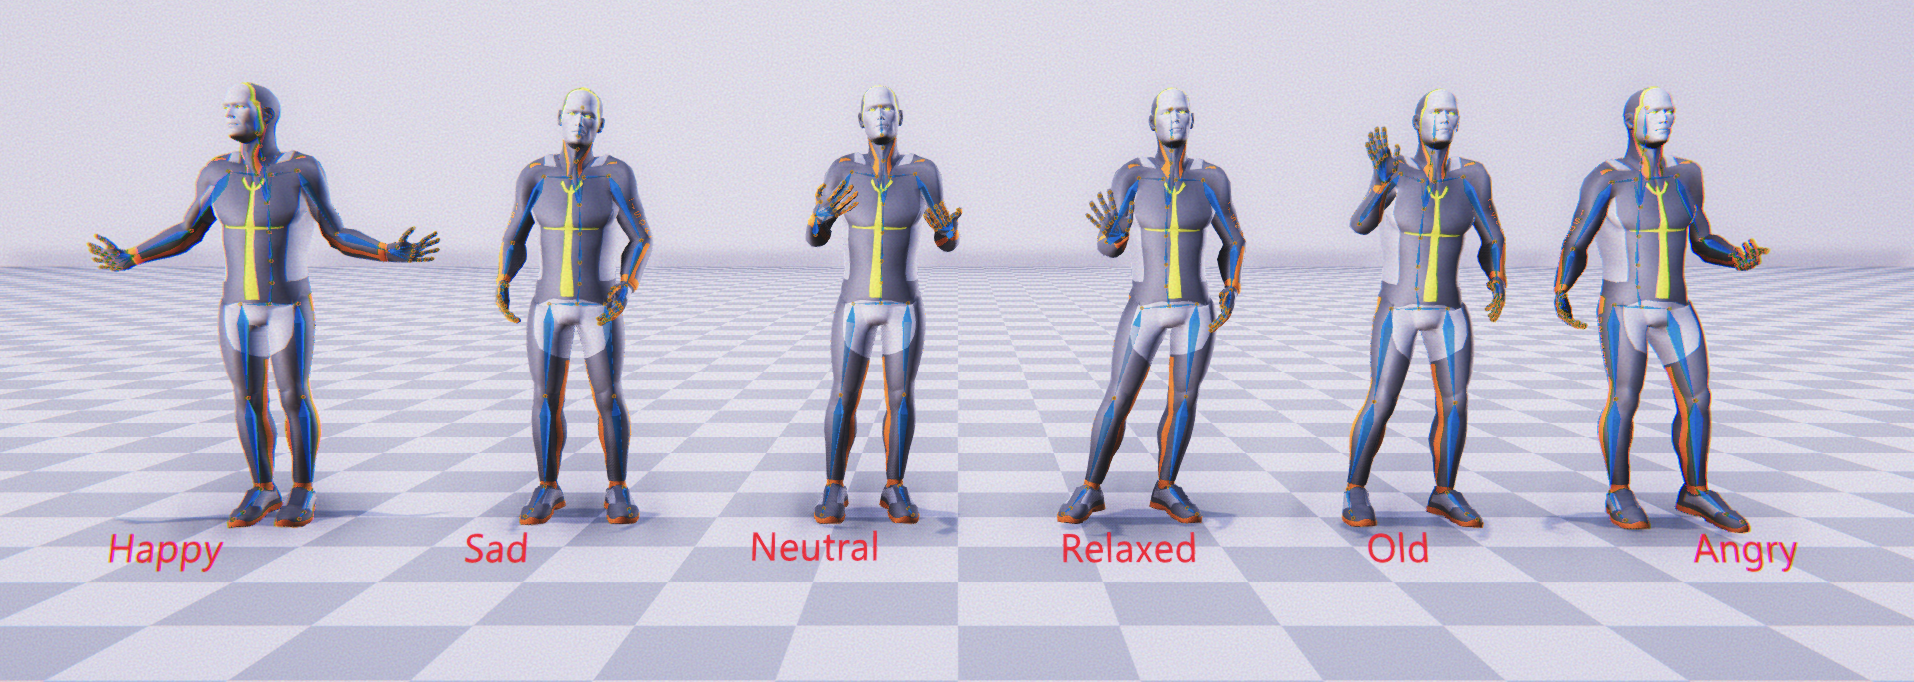
\includegraphics[width=\textwidth]{EmotionAnimation}
	\caption{Minh hoạ về 6 cử chỉ $\texttt{Happy}$, $\texttt{Sad}$, $\texttt{Neutral}$, $\texttt{Old}$, $\texttt{Relaxed}$ và $\texttt{Angry}$}
\end{figure}

Chúng tôi sử dụng tập dữ liệu ZeroEGGS \cite{ghorbani2022zeroeggszeroshotexamplebasedgesture} là một bộ dữ liệu motion capture được xây dựng để nghiên cứu và phát triển các mô hình tạo cử chỉ. Nó bao gồm 67 đoạn độc thoại do diễn viên motion capture nữ thực hiện, với tổng thời gian là 135 phút. Các đoạn hội thoại trong tập dữ liệu được biểu diễn với 6 cảm xúc khác nhau: $\texttt{Happy}$, $\texttt{Sad}$, $\texttt{Neutral}$, $\texttt{Old}$, $\texttt{Relaxed}$ và $\texttt{Angry}$, giúp mô phỏng nhiều trạng thái cảm xúc khác nhau trong cử chỉ và chuyển động cơ thể. ZeroEGGS cung cấp một nền tảng phong phú để nghiên cứu khả năng kết hợp giữa bài nói và cử chỉ động, phục vụ cho việc tạo ra các mô hình có thể điều chỉnh cử chỉ tương ứng với cảm xúc và ngữ nghĩa của văn bản.

\section{Quá trình xử lý dữ liệu}

Dữ liệu chúng tôi bao gồm các tệp tin BVH (BioVision Motion Capture) được thu nhận từ các cảm biến bằng các hệ thống Motion Capture. 


\textbf{Hierachy}: bao gồm 75 Bone $\{ \mathbf{t}_i \}^{75} $, có vị trí ban đầu  $\mathbf{t}_{i} = \{t_x, t_y, t_z\}$


\vspace{5pt}


\textbf{Motion}:
Bone trong dữ liệu BVH bao gồm vị trí $\mathbf{position}_{\operatorname{local}}  \in \mathbb{R}^{3}$ và góc quay $\mathbf{rotation}_{\operatorname{local}} \in \mathbb{R}^{3}$.

Chúng tôi chuyển dữ liệu từ góc quay Euler sang góc quay Quaternion, với góc quay Quaternion là một số phức gồm 3 số phức. 

Quá trình này được trình bày ở phụ lục \ref{Appendix2}

\section{Quá trình huấn luyện}

Toàn bộ quá trình huấn luyện mô hình được thực hiện trong vòng 1 ngày với các tham số sau: số bước huấn luyện $T = 1000$, sử dụng GPU Nvidia 3090, và chia tập dữ liệu theo tỷ lệ $8:1:1$ cho các tập training, testing và validation. Learning rate được thiết lập là $3 \times 10^{-5}$, với batch size là 384 và tổng cộng 300,000 mẫu. Quá trình huấn luyện được triển khai trên mã nguồn chương trình có sẵn tại: \hyperlink{https://github.com/hmthanh/OHGesture}{hmthanh/OHGesture} .


\section{Quá trình sử dụng Unity để kết xuất}

Để trực quan hóa quá trình sinh cử chỉ từ dữ liệu đầu ra của mô hình, chúng tôi sử dụng Unity, kết thừa mã nguồn từ mô hình DeepPhase \cite{starke2022deepphase}  . Dữ liệu sau khi sinh là file BVH (BioVision Motion Capture), trong Unity chúng tôi bổ sung mã nguồn CSharp để kết xuất theo vị trí toạ độ và nhãn tương ứng, với vị trí và góc quay của các xương được biểu diễn dưới dạng quaternion.

Chi tiết phần render cử chỉ được sinh ra, tôi trình bày ở phụ lục \ref{Appendix3}.

Mã nguồn chương trình Unity được chúng tôi công khai ở \hyperlink{https://github.com/DeepGesture/deepgesture-unity}{DeepGesture/DeepGesture-Unity}
%
%
\section{Phương pháp đánh giá}
\label{sec:evaluation}

Quá trình đánh giá được thực hiện qua hai độ đo chính là: Mean Opinion Scores (MOS) và Fréchet Inception Distance (FID).

\subsection{Mean Opinion Scores (MOS)}

Hiện tại, chưa có một độ đo chung cho bài toán sinh cử chỉ, đặc biệt là sinh cử chỉ từ âm thanh, vì vậy chúng tôi dựa vào đánh giá chủ quan của con người để thực hiện các đánh giá thực nghiệm. 
Tương tự như các phương pháp trước đây \cite{yoon2022genea}; \cite{kucherenko2021large}; các mô hình sinh cử chỉ điều khiển bằng giọng nói vẫn thiếu các chỉ số mục tiêu phản ánh một cách nhất quán với nhận thức chủ quan của con người  \cite{alexanderson2022listen}.
MOS được đo lường thông qua ba tiêu chí:

\begin{itemize}
	\item Human-likeness (Mức độ giống con người)
	\item Gesture-Speech Appropriateness (Sự phù hợp giữa cử chỉ và lời nói)
	\item Gesture-style Appropriateness (Sự phù hợp giữa phong cách cử chỉ)
\end{itemize}


\subsection{Fréchet Inception Distance (FID)}
FID đo sự tương đồng về phân phối giữa cử chỉ sinh ra $\mathbf{g}$ và cử chỉ thực tế $\mathbf{r}$. Công thức tính FID là:

\begin{equation}
	\text{FID} = \left\| \mu_r - \mu_g \right\|^2 + \operatorname{Tr}\left( \Sigma_r + \Sigma_g - 2 \sqrt{\Sigma_r \Sigma_g} \right)
\end{equation}

%\begin{itemize}
%	\item $\mu_r$ và $\Sigma_r$ là vector trung bình và ma trận hiệp phương sai của đặc trưng từ dữ liệu thực tế (real gestures).
%	\item $\mu_g$ và $\Sigma_g$ là vector trung bình và ma trận hiệp phương sai của đặc trưng từ cử chỉ tổng hợp (generated gestures).
%	\item $\|\mu_r - \mu_g\|^2$ là bình phương khoảng cách Euclidean giữa các vector trung bình.
%	\item $\text{Tr}\left( \Sigma_r + \Sigma_g - 2\sqrt{\Sigma_r \Sigma_g} \right)$ là trace của ma trận hiệp phương sai kết hợp, đo lường sự khác biệt giữa hai phân phối Gaussian.
%\end{itemize}

Trong đó:

\begin{itemize}
	\item $\mu$: Trung bình các đặc trưng của cử chỉ.
	\item $\Sigma$: Ma trận hiệp phương sai của đặc trưng.
	\item $\operatorname{Tr}$: Tổng đường chéo chính của ma trận hiệp phương sai.
	\item $\sqrt{\Sigma_r \Sigma_g}$: Sự tương đồng giữa các phân phối cử chỉ thực tế và cử chỉ sinh ra.
\end{itemize}

FID thấp cho thấy phân phối của cử chỉ sinh ra gần giống với cử chỉ thực tế, trong khi FID cao gợi ý sự khác biệt lớn, cho thấy chất lượng cử chỉ sinh ra kém hơn.



%\begin{itemize}
	%		\item \textbf{FID thấp}: Cho thấy phân phối của cử chỉ sinh ra rất gần với phân phối của cử chỉ thực tế, tức là cử chỉ tổng hợp trông tự nhiên hơn.
	%		\item \textbf{FID cao}: Gợi ý rằng các cử chỉ sinh ra khác biệt nhiều so với các cử chỉ thực tế, tức là chất lượng kém hơn.
	%	\end{itemize}
%	




% ngay cả với Fréchet gesture distance (FGD) \cite{yoon2022genea}, \cite{dabral2023mofusion}. Vì vậy, tất cả các điểm số thực nghiệm trong nghiên cứu này được thực hiện thông qua đánh giá chủ quan của con người. Chúng tôi đánh giá trên ba tiêu chí: độ giống con người, sự phù hợp giữa cử chỉ và giọng nói, và sự phù hợp giữa cử chỉ và phong cách. Các tiêu chí này được lấy từ đánh giá trong GENEA \cite{yoon2022genea}.


%Chúng tôi so sánh mô hình đề xuất của chúng tôi với StyleGestures \cite{alexanderson2020style}, Audio2Gestures \cite{li2021audio2gestures}, ExampleGestures \cite{ghorbani2022zeroeggszeroshotexamplebasedgesture}.

\section{So sánh với các phương pháp hiện tại}
\label{sec:result}


Ở đây chúng tôi sử dụng lại kết quả đánh giá của mô hình baseline \textbf{DiffuseStyleGesture} \cite{yang2023diffusestylegesture} trong độ đo về  cảm nhận đánh giá của con người do lĩnh vực sinh cử chỉ vẫn còn rất mới, chi phí để ước lượng các mô hình còn lớn nên chúng tôi không thể đánh giá được mô hình OHGesture. Vì vậy các kết quả này chưa bao gồm thông tin kết qủa về mô hình \textbf{OHGesture} mà chúng tôi đề xuất.

\begin{figure}[htbp]
	\centering
	\begin{subfigure}[b]{0.3\textwidth}
		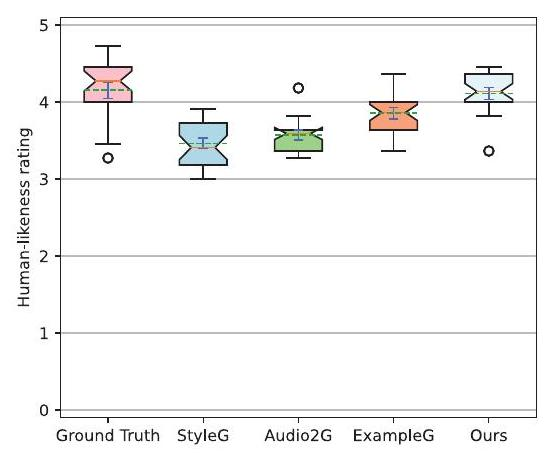
\includegraphics[width=\textwidth]{humanlike_score.jpg}
		\caption*{(a) Human-likeness}
	\end{subfigure}
	\hfill
	\begin{subfigure}[b]{0.3\textwidth}
		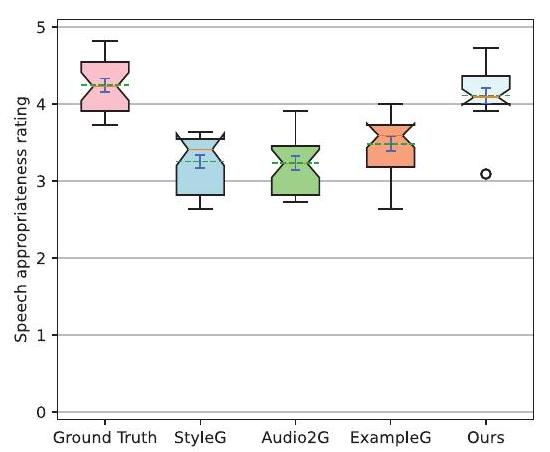
\includegraphics[width=\textwidth]{speech_score.jpg}
		\caption*{\small (b) Speech Appropriateness}
	\end{subfigure}
	\hfill
	\begin{subfigure}[b]{0.3\textwidth}
		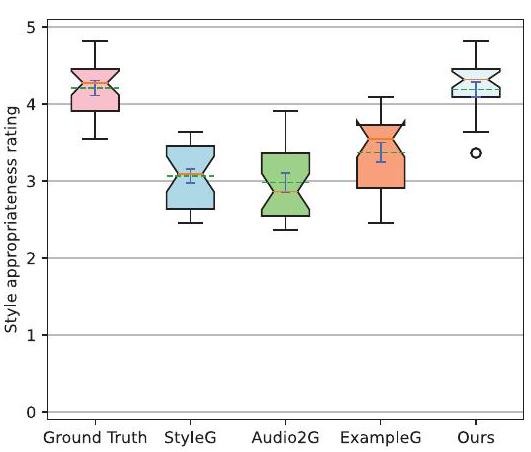
\includegraphics[width=\textwidth]{style_score.jpg}
		\caption*{(c) Style Appropriateness}
	\end{subfigure}
	
	%	    \caption[Biểu đồ hộp mô tả kết quả so sánh MOS]{Biểu đồ hộp mô tả kết quả so sánh MOS cho các mô hình khác nhau trong các chiều khác nhau. Hộp mở rộng từ phân vị thứ nhất thấp nhất (Q1) đến phân vị thứ ba lớn nhất (Q3) của dữ liệu. Đường đỏ chỉ là giữa. Các khe nhỏ biểu thị khoảng tin cậy $95\%$ (CI) xung quanh giữa. Khi CI nhỏ hơn Q1 hoặc lớn hơn Q3, khe mở rộng ra khỏi hộp, tạo ra một hình dáng "lật" độc đáo. Chúng tôi cũng đã đánh dấu giá trị trung bình và khoảng tin cậy $95\%$ của nó trong hình với đường nét đứt màu xanh lá cây và đường dọc màu xanh lam, tương ứng.}
	\label{fig:compare }
\end{figure}


Để hiểu hiệu suất thị giác thực tế của phương pháp của chúng tôi, chúng tôi tiến hành một nghiên cứu người dùng so sánh các cử chỉ được tạo ra từ phương pháp của chúng tôi và dữ liệu chụp chuyển động thực tế. Độ dài của các đoạn clip đánh giá dao động từ 11 đến 51 giây, với độ dài trung bình là 31.6 giây, dài hơn so với các đoạn trong đánh giá GENEA \cite{yoon2022genea} (8-10 giây), vì thời gian dài hơn có thể tạo ra kết quả rõ ràng và thuyết phục hơn \cite{yang2022reprgesture}. Người tham gia đánh giá trên thang điểm từ 5 đến 1, với các nhãn từ $\texttt{excellent}$,  $\texttt{good}$, $\texttt{fair}$, $\texttt{poor}$, đến $\texttt{bad}$. 


\begin{table}[!t]
	\centering
		\begin{tabular}{lcc}
			\hline
			\multicolumn{1}{c}{Name} &
			\begin{tabular}[c]{@{}c@{}}Human\\ likeness \end{tabular}$\uparrow$ &
			\begin{tabular}[c]{@{}c@{}}Gesture-speech\\ appropriateness\end{tabular}$\uparrow$ \\ \hline
			Ground Truth          & 4.15 $\pm$ 0.11          & 4.25 $\pm$ 0.09          \\
			Ours                  & \textbf{4.11 $\pm$ 0.08} & \textbf{4.11 $\pm$ 0.10} \\
			\quad$-$ WavLM             & 4.05 $\pm$ 0.10          & 3.91 $\pm$ 0.11          \\
			\quad$-$ Cross-local attention   & 3.76 $\pm$ 0.09          & 3.51 $\pm$ 0.15          \\
			\quad$-$ Self-attention    & 3.55 $\pm$ 0.13          & 3.08 $\pm$ 0.10          \\
			% \begin{tabular}[c]{@{}c@{}}$-$ attention (GRU based) \\ (GRU based)\end{tabular} &
			\quad$-$ Attention + GRU&
			3.10 $\pm$ 0.11 &
			2.98 $\pm$ 0.14 \\
			\quad$+$ Forward attention & 3.75 $\pm$ 0.15          & 3.23 $\pm$ 0.24          \\
			\hline
		\end{tabular}
	\caption{Kết quả của các nghiên cứu loại bỏ (Ablation studies). "$-$" chỉ các mô-đun không được sử dụng và "$+$" chỉ các mô-đun bổ sung. Chữ in đậm chỉ ra chỉ số tốt nhất.}
	\label{Ab}
\end{table}


\section{Xây dựng và tiêu chuẩn hoá hệ thống đánh giá kết quả sinh cử chỉ}

Hiện nay các mô hình sinh (gesture generation) cử chỉ được quan tâm nghiên cứu với rất nhiều mô hình khác nhau, tuy nhiên do không có độ đo chung, vì các độ đo truyền thống như FID (Fréchet Inception Distance) hay IS (Inception Score),.. không thể hiện được hết các tính chất Giống người (Human-likeness), tính phù hợp với giọng nói (Speech Appropriateness), và tính phù hợp với phong cách (Style Appropriateness) của cử chỉ. Các mô hình cũng được thực hiện và huấn luyện trên một tập dữ liệu khác nhau, vì vậy rất khó để biết được mô hình nào đã đạt kết quả tốt hơn, và mô hình nào là state-of-the-art, từ đó khó có thể đạt được sự tiến bộ trong lĩnh vực sinh cử chỉ. Việc thiếu tiêu chuẩn chung để đánh giá trong cộng đồng nghiên cứu khiến chúng tôi mong muốn xây dựng một hệ thống xếp hạng trực tuyến \cite{nagy2024towards} \hyperlink{https://genea-workshop.github.io/leaderboard/}{GENEA Leaderboard}, là một bảng xếp hạng các mô hình sinh cử chỉ. Chúng tôi thu thập và xử lý một tập dữ liệu cử chỉ từ nhiều ngôn ngữ và từ nhiều tập dữ liệu khác nhau và tiêu chuẩn hoá để tạo ra một tập dữ liệu duy nhất.  Sau đó, chúng tôi sẽ mời các tác giả của các mô hình để học và dự đoán trên tập dữ liệu đã được tiêu chuẩn hoá, sau khi có kết quả sinh cử chỉ, chúng tôi sẽ thuê những người tham gia nghiên cứu trên Prolific để đánh giá và xếp hạng kết quả sinh cử chỉ của các mô hình. Hiện tại chúng tôi đang xây dựng hệ thống trực tuyến \hyperlink{https://github.com/hemvip/hemvip.github.io}{hemvip/hemvip.github.io} với mục tiêu đánh giá kết quả sinh của cử chỉ thông qua việc thuê các người tham gia đánh giá kết quả thông qua Prolific. Chúng tôi sẽ bổ sung các đánh giá về mô hình OHGesture dựa trên các điểm số trên.

Thông qua hệ thống đánh giá này, nghiên cứu kỳ vọng sẽ thiết lập một tiêu chuẩn chung, từ đó tạo động lực cho sự tiến bộ trong lĩnh vực sinh cử chỉ.

%Chi tiết về nghiên cứu người dùng có thể được tìm thấy trong tư liệu bổ sung.

%Điểm số ý kiến trung bình (MOS) về độ giống con người, sự phù hợp giữa cử chỉ và giọng nói, và sự phù hợp giữa cử chỉ và phong cách được báo cáo trong \ref{fig}. 
%Nếu các góc của hai hộp không chồng lên nhau, điều này chứng tỏ rằng các phân phối khác biệt đáng kể \cite{mcgill1978variations}. Phương pháp của chúng tôi vượt trội so với các phương pháp tiên tiến được so sánh trong cả ba chiều đánh giá, và thậm chí tạo ra các kết quả cạnh tranh với dữ liệu thực tế. Phản hồi từ người tham gia cho thấy cử chỉ do phương pháp của chúng tôi tạo ra "có ý nghĩa ngữ nghĩa hơn", "tự nhiên hơn", và "phù hợp với phong cách", mặc dù có một số vấn đề về "chuyển động trượt chân" so với Dữ liệu Thực. Tuy nhiên, đây là một vấn đề phổ biến đối với các hệ thống tạo ra chuyển động không dựa trên vật lý và có thể được giải quyết thông qua xử lý sau \cite{ghorbani2022zeroeggszeroshotexamplebasedgesture}, \cite{luvizon2023scene}.

%Hiện tại chưa có một độ đo chung cho bài toán sinh cử chỉ, đặc biệt là sinh cử chỉ từ âm thanh, vì vậy chúng tôi 
%các cử chỉ điều khiển bằng giọng nói thiếu các chỉ số mục tiêu phản ánh một cách nhất quán với nhận thức chủ quan của con người \cite{yoon2022genea}; \cite{kucherenko2021large}; \cite{alexanderson2022listen}, ngay cả với Fréchet gesture distance (FGD) \cite{yoon2022genea}, \cite{dabral2023mofusion}, do đó tất cả các điểm số thực nghiệm của chúng tôi được thực hiện thông qua đánh giá chủ quan của con người. Chúng tôi thực hiện đánh giá trên ba chiều. Hai chiều đầu tiên theo đánh giá trong GENEA \cite{yoon2022genea}, bao gồm đánh giá về độ giống con người và sự phù hợp giữa cử chỉ và giọng nói. Chiều thứ ba là sự phù hợp giữa cử chỉ và phong cách.
%
%Nghiên cứu Người Dùng. Để hiểu về hiệu suất thị giác thực tế của phương pháp của chúng tôi, chúng tôi tiến hành một nghiên cứu người dùng giữa các trình tự cử chỉ được tạo ra bởi mỗi phương pháp được so sánh và dữ liệu chụp chuyển động thực. Độ dài của các đoạn clip được đánh giá dao động từ 11 đến 51 giây, với độ dài trung bình là 31.6 giây. Lưu ý rằng các cử chỉ clip được sử dụng cho đánh giá chủ quan ở đây dài hơn so với đánh giá GENEA \cite{yoon2022genea} (8-10 giây), vì một khoảng thời gian dài có thể tạo ra kết quả phù hợp rõ ràng và thuyết phục hơn \cite{yang2022reprgesture}. Người tham gia đánh giá trên một khoảng điểm từ 5 đến 1, với các nhãn (tốt nhất đến tệ nhất) là "tuyệt vời," "tốt," "công bằng," "kém," và "tệ." Thêm chi tiết về nghiên cứu người dùng được hiển thị trong tư liệu bổ sung.
%
%
%
%
%
%
%Điểm số ý kiến trung bình (MOS) về độ giống con người, phù hợp giọng nói và phù hợp phong cách được báo cáo trong \ref{fig:mosscore}. Nếu các góc của hai hộp không chồng lên nhau, chúng ta có thể coi đây là bằng chứng mạnh mẽ rằng các phân phối khác nhau đáng kể \cite{mcgill1978variations}. Phương pháp của chúng tôi vượt trội đáng kể so với các phương pháp tiên tiến được so sánh với độ giống con người, phù hợp giữa cử chỉ và giọng nói, cũng như phù hợp giữa cử chỉ và phong cách, và thậm chí tạo ra các kết quả cạnh tranh với dữ liệu thực tế ở cả ba chiều. Theo phản hồi từ người tham gia, cử chỉ được tạo ra bởi chúng tôi "có ý nghĩa ngữ nghĩa hơn", "tự nhiên hơn," và "phù hợp với phong cách," trong khi phương pháp của chúng tôi có "chuyển động trượt chân" so với Dữ liệu Thực. Tuy nhiên, đây là một vấn đề phổ biến đối với các hệ thống tạo ra chuyển động không dựa trên vật lý và có thể được giải quyết thông qua xử lý sau \cite{ghorbani2022zeroeggszeroshotexamplebasedgesture}, \cite{luvizon2023scene}.

%\begin{table}[t]
%	\centering
%	\caption{Impact of the positional encoding block.}
%	\label{tab:pos_enc}
%	
%	\newcolumntype{Y}{>{\raggedleft\arraybackslash}X}
%	\newcolumntype{Z}{>{\centering\arraybackslash}X}
%%	\begin{tabularx}{\linewidth}{XlYY}
%	
%%		
%	
%%		\bottomrule
%%		\begin{tabularx}{\linewidth}{XlYY}
%%		\toprule
%%		Dataset & System & FGD $\downarrow$ & PMB ($\%$) $\uparrow$ \\
%%		\toprule
%%		\multirow{2}{*}{TED} & Without positional encoding & 2.19 & 88.13 \\
%%		& With positional encoding & $\bm{2.04}$ & $\bm{89.52}$ \\
%%		\bottomrule
%%		\end{tabularx}
%
%
%
%
%% \begin{tabularx}{\linewidth}{XlYY}
%%	\toprule
%%	Dataset & System & FGD $\downarrow$ & PMB ($\%$) $\uparrow$ \\
%%	\toprule
%%	\multirow{2}{*}{TED} & encoding & 2.19 & 88.13 \\
%%	& With positional encoding & $2.04$ & $89.52$ \\
%%	\bottomrule
%%\end{tabularx}
%
%
%
%%		\multirow{2}*{Trinity} & Without positional encoding & 11.15 & 89.98 \\
%%				& With positional encoding & $\bm{10.78}$ & $\bm{91.36}$ \\
%%\hline
%%This is a long entry that will automatically adjust its width. & Short text & Another long entry that will also adjust its width. \\
%%\hline
%%More text & Another short entry & Yet another long entry to demonstrate text wrapping and width adjustment. \\
%%\hline
%
%\end{table}



% \section{Đánh Giá}
% \label{sec:experiments}
 % Khả năng Kiểm soát Cử chỉ

%\subsection{Khả năng kiểm soát cử chỉ}
%\label{subsec:stylecontrol}

%Giả sử rằng âm thanh trung tính không ảnh hưởng đến phong cách của cử chỉ, chúng ta có thể tạo ra các cử chỉ được phong cách hóa với một bài nói trung tính bằng cách đặt $\gamma=1$ và $e$ trong \ref{eq:denoise}. Chúng tôi chọn hai đoạn hội thoại trong tập kiểm thử với âm thanh trung tính để tạo ra sáu cử chỉ được phong cách hóa tương ứng. \ref{fig:emotiondataset} minh họa cử chỉ được tạo ra $\hat{\mathbf{x}}_{t}$ của các phong cách đầu vào $s$ khác nhau với cùng một âm thanh trung tính được thị giác hóa bằng phương pháp tSNE.
%
%\begin{figure}
%    \centering
%    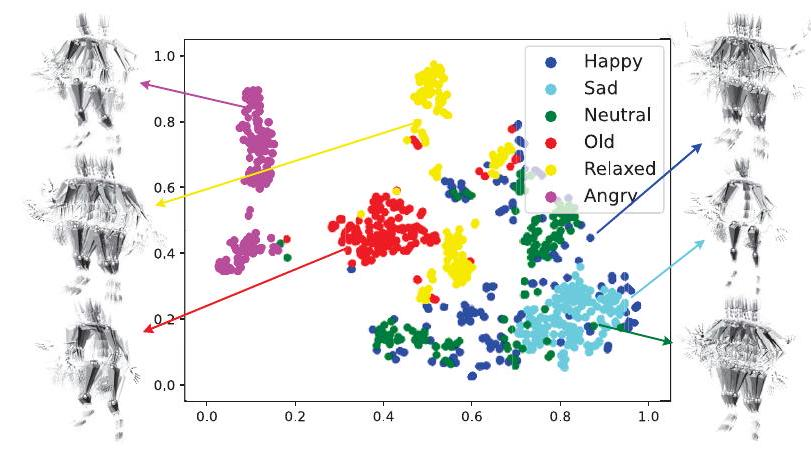
\includegraphics[width=0.7\linewidth]{images/emotion_dataset.jpg}
%    \caption[Biểu đồ tSNE với các phong cách khác nhau]{Hiển thị tSNE của các cử chỉ với các phong cách khác nhau và bản đồ bóng của cử chỉ xương cơ với phong cách tương ứng. Ví dụ, với cử chỉ 'Old', hông và đầu gối của nó uốn cong hơn, và tay của nó cơ bản nằm ở đầu gối hoặc hông.}
%    \label{fig:emotiondataset}
%\end{figure}
%
%Chúng tôi cũng vẽ biểu đồ xương cơ được tạo ra bởi phong cách tương ứng trong hình, và có thể thấy rằng đối với phong cách 'Old', hông và đầu gối của nó uốn cong hơn, và tay của nó cơ bản nằm ở đầu gối hoặc hông; với phong cách 'Sad', đầu của nó đang nghiêng và tay nó ở một vị trí thấp hơn; với phong cách 'Relax', hông của nó đang chuyển lên phía trước và tư thế đứng của nó là thoải mái; với phong cách 'Angry', tay của nó di chuyển lên và xuống nhanh chóng. Lưu ý rằng mặc dù sự khác biệt giữa cử chỉ phong cách 'trung tính' và 'Happy' vẫn khá rõ ràng trong việc thị giác hóa phong cách của xương cơ, tức là với phong cách 'Happy', vị trí tay của nó là cao hơn và biên độ của nó lớn hơn, tuy nhiên tSNE của chúng gần như kết hợp với nhau. Trong phân tích của chúng tôi, điều này xảy ra vì bài nói trung tính gọi là vẫn chứa thông tin như cảm xúc và ngữ nghĩa mà có trong các đặc trưng WavLM. Sự cân bằng giữa phong cách từ âm thanh $\mathbf{a}$ và từ phong cách $\mathbf{e}$ có thể được kiểm soát thêm bằng cách chỉnh sửa cường độ phong cách $\gamma$.
%
%Giả sử rằng âm thanh Neutral không ảnh hưởng đến cảm xúc của cử chỉ, chúng ta có thể tạo ra các cử chỉ được điều chỉnh theo cảm xúc với một bài nói Neutral bằng cách đặt $\gamma=1$ và $e$ trong \ref{eq:denoise}. Chúng tôi chọn hai đoạn hội thoại trong tập kiểm thử với âm thanh trung tính để tạo ra sáu cử chỉ được điều chỉnh cảm xúc tương ứng. Hình \ref{fig:emotiondataset} minh họa cử chỉ được tạo ra $\hat{\mathbf{x}}_{t}$ cho các cảm xúc đầu vào $s$ khác nhau với cùng một âm thanh trung tính, được thị giác hóa bằng phương pháp t-SNE.
%
%\begin{figure}
%	\centering
%	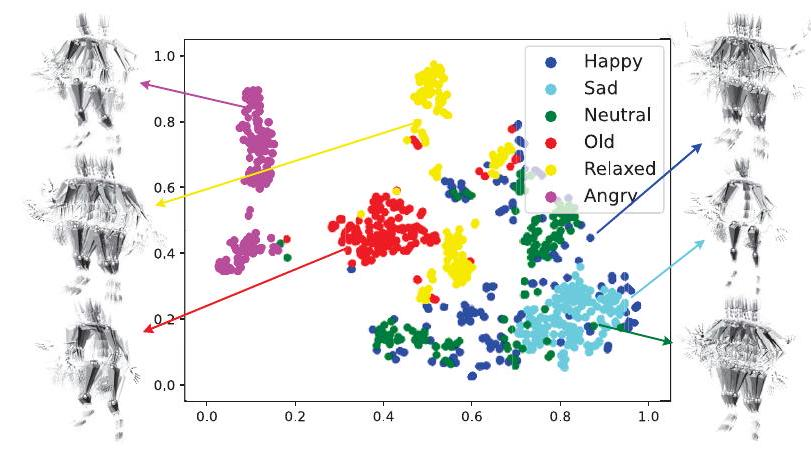
\includegraphics[width=0.7\linewidth]{images/emotion_dataset.jpg}
%	\caption[Biểu đồ t-SNE với các cảm xúc khác nhau]{Hiển thị t-SNE của các cử chỉ với các cảm xúc khác nhau và bản đồ bóng của cử chỉ xương cơ với cảm xúc tương ứng. Ví dụ, với cử chỉ 'Old', hông và đầu gối của nó uốn cong hơn, và tay của nó cơ bản nằm ở gần đầu gối hoặc hông.}
%	\label{fig:emotiondataset}
%\end{figure}
%
%Chúng tôi cũng biểu diễn các cử chỉ khung xương tương ứng với từng cảm xúc trong hình và nhận thấy rằng đối với cảm xúc 'Old', hông và đầu gối có độ uốn cong lớn hơn, và tay chủ yếu nằm ở đầu gối hoặc hông; với cảm xúc 'Sad', đầu nghiêng và tay ở vị trí thấp hơn; với cảm xúc 'Relaxed', hông hơi hướng về phía trước với tư thế đứng thoải mái; với cảm xúc 'Angry', tay chuyển động nhanh chóng lên xuống. Lưu ý rằng mặc dù sự khác biệt giữa cử chỉ với cảm xúc 'Neutral' và 'Happy' vẫn rõ ràng khi thị giác hóa khung xương, cụ thể là với cảm xúc 'Happy', tay ở vị trí cao hơn và biên độ lớn hơn, nhưng các điểm t-SNE của chúng lại gần nhau. Trong phân tích của chúng tôi, điều này là do bài nói trung tính vẫn chứa thông tin về cảm xúc và ngữ nghĩa từ các đặc trưng của WavLM. Sự cân bằng giữa cảm xúc từ âm thanh $\mathbf{a}$ và từ điều chỉnh cảm xúc $\mathbf{e}$ có thể được kiểm soát thêm thông qua việc điều chỉnh cường độ cảm xúc $\gamma$.



%\subsection{Khả năng điều chỉnh cảm xúc của cử chỉ}
%
%
%\begin{figure}
%	\centering
%	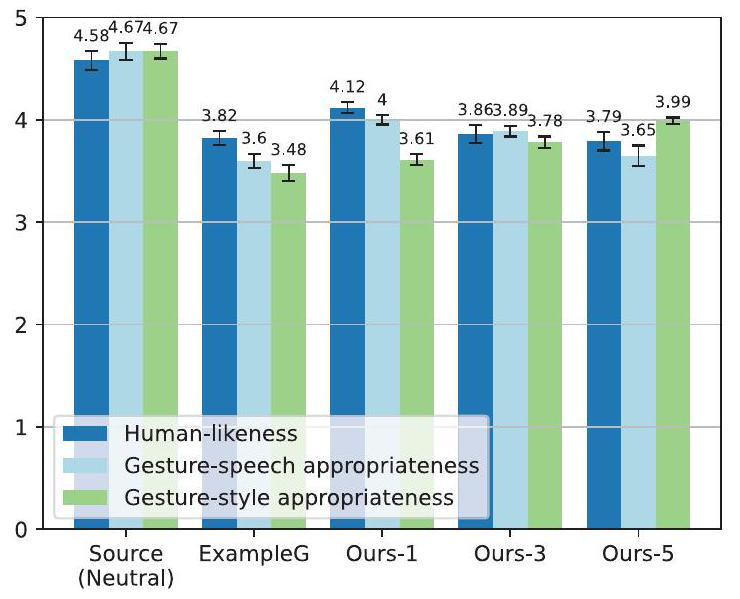
\includegraphics[width=0.7\linewidth]{images/mos_score.jpg}
%	\label{fig:mosscore}
%	\caption{Kết quả trung bình của MOS}
%	
%	%    \caption[Kết quả trung bình của MOS]{Kết quả trung bình của MOS với khoảng tin cậy $95\%$ cho ba chiều. 'Ours-$\gamma$' chỉ ra cường độ kiểm soát phong cách $\gamma$ của mô hình của chúng tôi. Mô hình của chúng tôi vượt trội đáng kể so với ExampleGesture tổng thể và có thể chỉnh sửa cường độ của các phong cách. Tham số $\gamma$ tăng và hai điểm số còn lại sẽ giảm một cách hợp lý.}
%	
%	\vspace{-10pt}
%\end{figure}

%Trong nghiên cứu này, chúng tôi điều chỉnh cường độ cảm xúc của cử chỉ thông qua tham số $\gamma$, với các giá trị $\gamma=1$ và $\gamma=3$ cho cảm xúc 'Happy' và 'Old'. Khi $\gamma=3$, cảm xúc 'Happy' tạo ra cử chỉ mạnh mẽ với chuyển động tay và cơ thể rõ rệt, trong khi 'Old' thể hiện cử chỉ ít năng động hơn, với hông ít uốn cong và tay ít được nâng lên. Các giá trị $\gamma$ khác cho phép điều chỉnh cường độ cảm xúc, giúp tạo ra cử chỉ tương ứng với các cảm xúc chuyển tiếp giữa 'Happy' và 'Old'. Các thử nghiệm cho thấy rằng việc tăng $\gamma$ giúp tạo ra cử chỉ phù hợp với cảm xúc mong muốn, ngay cả khi chúng không có trong dữ liệu huấn luyện. 
%Một nghiên cứu người dùng cho thấy mô hình của chúng tôi vượt trội so với ExampleGesture trong việc điều chỉnh cường độ cảm xúc và tạo ra cử chỉ tự nhiên và phù hợp với ngôn ngữ.
%
%Để phân tích chi tiết hơn mối quan hệ giữa cường độ cảm xúc và cảm xúc mà bài nói ngụ ý, chúng tôi lựa chọn hai cảm xúc là 'Happy' và 'Old' và thiết lập $\gamma=1$ và $3$ trong \ref{eq:denoise}. Để so sánh kết quả, chúng tôi cũng thiết lập $\gamma=0.5$ trong \ref{eq:denoise} để nội suy giữa các cảm xúc khác nhau. Các tham số còn lại được giữ nguyên, và chúng tôi biểu diễn cử chỉ được tạo ra trong 12 giây với FPS $=1$.
%
%Có thể quan sát thấy rằng khi sử dụng cảm xúc 'Happy' với $\gamma=3$, chuyển động cơ thể và cử động tay đều đạt cường độ cao nhất, và vị trí tay được nâng cao nhất; ngược lại, khi sử dụng cảm xúc 'Old' với $\gamma=3$, hông có độ uốn cong lớn nhất, tay ít được nâng lên, và chuỗi chuyển động nhìn chung có ít thay đổi. Đối với ba kết quả còn lại, cường độ cảm xúc nằm giữa hai trường hợp này, với cảm xúc dần chuyển từ Happy sang Old. Kiến trúc mô hình của chúng tôi giúp cử chỉ và bài nói kết hợp với nhau hài hòa hơn, dù hai cảm xúc không hoàn toàn giống nhau. Lưu ý rằng khi sử dụng cảm xúc 'Happy' và 'Old' với $\gamma=0.5$, kết quả gần giống như khi sử dụng cảm xúc 'Happy' với $\gamma=1$, trong khi cảm xúc 'Old' khó nhận ra. Quan sát này khẳng định kết luận trước đó rằng cảm xúc 'Happy' đã được thể hiện trong bài nói 'Neutral' dùng để kiểm thử. Điều này cho thấy, chẳng hạn, trong các thử nghiệm của chúng tôi, nếu muốn điều chỉnh bài nói 'Happy' để tạo ra cử chỉ 'Sad', $\gamma=1$ có thể không hiệu quả do mô hình có xu hướng học cảm xúc Happy từ bài nói. Do sự tương quan giữa cảm xúc của bài nói và cảm xúc của cử chỉ, việc tăng giá trị $\gamma$ có thể giúp điều chỉnh cảm xúc tốt hơn, cho phép tạo ra các cử chỉ không có trong tập dữ liệu gốc (ví dụ: cử chỉ cho bài nói 'Happy' nhưng có cảm xúc 'Sad') thông qua việc điều chỉnh cường độ cảm xúc.
%
%Hơn nữa, để tìm hiểu mối quan hệ giữa cường độ cảm xúc với độ giống con người (human-likeness) và sự phù hợp với ngôn ngữ, chúng tôi đã tiến hành một nghiên cứu người dùng. Để tránh ảnh hưởng của cảm xúc trong ngôn ngữ nói đến đánh giá của người tham gia, tương tự như trước, chúng tôi chỉ điều chỉnh cường độ cảm xúc cho một bài nói Neutral và yêu cầu người tham gia đánh giá theo ba tiêu chí đặc trưng trước đó. ExampleGesture \cite{ghorbani2022zeroeggszeroshotexamplebasedgesture} cũng cho phép kiểm soát việc tạo ra các cảm xúc khác nhau từ cùng một bài nói, vì vậy chúng tôi chọn nó làm mô hình tham chiếu. Do các cử chỉ được tạo ra ở đây không tồn tại trong tập dữ liệu, bài nói Neutral với cảm xúc trung tính được sử dụng làm tham chiếu.

%
%\subsection{Khả năng chỉnh sửa Phong cách của cử chỉ}
%
%Để phân tích sâu hơn mối quan hệ giữa cường độ phong cách và phong cách được ngụ ý bởi bài nói, chúng tôi chọn phong cách 'Happy' và phong cách 'Old' và đặt $\gamma=1$ và 3 trong \ref{eq:denoise}. Ngoài ra, để so sánh kết quả, chúng tôi đặt $\gamma=0.5$ trong \ref{eq:denoise}, để nội suy giữa các phong cách khác nhau. Các tham số khác không thay đổi, và chúng tôi vẽ kết quả tạo ra cử chỉ trong 12 giây, với FPS $=1$.
%%như thể hiện trong 
%%\ref{fig:stylesample}.
%
%
%%Như thấy trong
%% \ref{fig:stylesample}, 
% Chúng ta có thể thấy rằng khi chúng ta sử dụng phong cách 'Happy' với $\gamma=3$, cả quá trình xoay cơ thể và chuyển động tay đều lớn nhất, và vị trí tay của nó là cao nhất; ngược lại, khi chúng ta sử dụng phong cách 'Old' với $\gamma=3$, hông của nó uốn cong nhất, tay hầu như không được nâng lên, và không có nhiều sự thay đổi trong toàn bộ chuỗi chuyển động; còn đối với ba kết quả khác, cường độ phong cách của chúng ở giữa hai trường hợp trên, và phong cách dần thay đổi từ vui vẻ đến già từ trên xuống dưới. Do kiến trúc mô hình của chúng tôi, cử chỉ và bài nói được tạo ra phù hợp hơn, mặc dù các phong cách này không giống nhau. Lưu ý rằng khi chúng ta sử dụng phong cách 'Happy' và 'Old' với $\gamma=0.5$, kết quả gần với việc sử dụng phong cách 'Happy' với $\gamma=1$, trong khi phong cách 'Old' gần như không thể cảm nhận được. Quan sát này tiếp tục xác nhận phát hiện trước đó rằng phong cách 'Happy' được nhúng trong bài nói 'trung tính' được sử dụng để kiểm thử. Phát hiện này hữu ích, ví dụ, chúng tôi đã phát hiện trong các thử nghiệm của mình rằng nếu chúng ta muốn kiểm soát bài nói 'Happy' để tạo ra cử chỉ 'Sad', $\gamma=1$ cơ bản là không hiệu quả vì mô hình có thể học được phong cách vui vẻ từ bài nói. Vì có sự liên kết giữa phong cách của bài nói và phong cách của cử chỉ, việc đặt $\gamma$ lớn hơn có thể chỉnh sửa phong cách tốt hơn. Do đó, chúng ta có thể tạo ra các cử chỉ không tồn tại trong tập dữ liệu gốc (ví dụ, cử chỉ cho bài nói 'Happy' nhưng có phong cách 'Sad') thông qua cường độ phong cách.
%
%
%% Nghiên cứu Người dùng. 
%Hơn nữa, chúng tôi muốn khám phá mối quan hệ giữa cường độ phong cách và độ giống con người cũng như sự phù hợp với ngôn ngữ, nên chúng tôi đã tiến hành một nghiên cứu người dùng. Để tránh phong cách trong ngôn ngữ nói ảnh hưởng đến việc đánh giá của người tham gia, giống như trước đó, chúng tôi chỉ kiểm soát cường độ của các phong cách cho một bài nói trung tính và sau đó yêu cầu người tham gia đánh giá ba chiều đặc trưng trước đó. ExampleGesture \cite{ghorbani2022zeroeggszeroshotexamplebasedgesture} cũng có thể kiểm soát việc tạo ra các phong cách khác nhau của các cử chỉ từ cùng một bài nói. Vì vậy, chúng tôi chọn nó làm mô hình tham chiếu. Vì các cử chỉ được tạo ra ở đây không tồn tại trong tập dữ liệu, bài nói trung tính với phong cách trung tính được sử dụng làm tham chiếu. 
%

%Kết quả được thể hiện trong hình \ref{fig:mosscore}.

%\begin{figure}
%    \centering
%    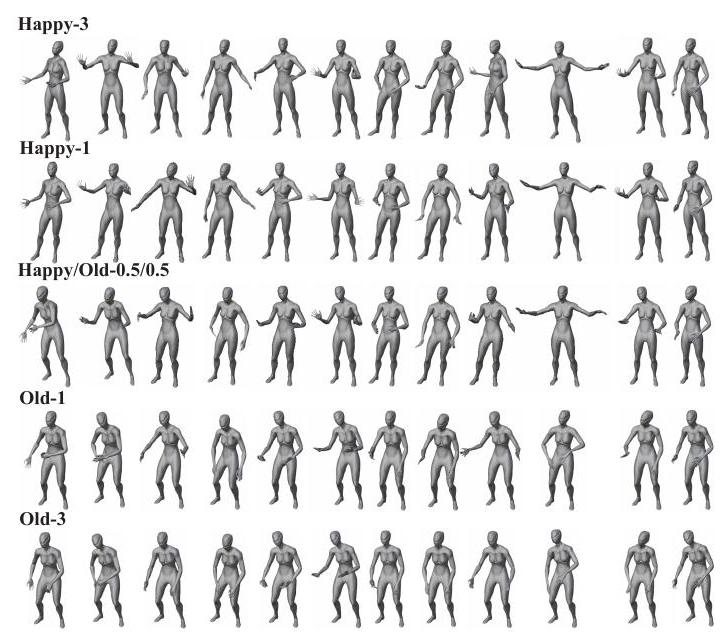
\includegraphics[width=0.6\linewidth]{images/style_sample.jpg}
%    \caption[Chỉnh sửa phong cách và nội suy]{\small Chỉnh sửa phong cách và nội suy. Từ trên xuống dưới, cơ thể xoắn và chuyển động tay dần giảm và vị trí tay trở nên thấp hơn. Mặc dù có sự thay đổi về phong cách, các cử chỉ được tạo ra vẫn khớp tốt với bài nói trong các phong cách khác nhau}
%    \label{fig:stylesample}
%\end{figure}


% % Hình 6: 



%Kết quả cho thấy rằng mô hình của chúng tôi tương tự như ExampleGesture về mặt phù hợp giữa phong cách cử chỉ của kết quả ở $\gamma=1$, và độ giống con người cũng như sự phù hợp với ngôn ngữ của chúng tôi vượt quá ExampleGesture. Trong khi đó, phong cách trở nên đáng kể hợp lý hơn khi $\gamma$ tăng, nhưng điểm của hai chiều khác giảm. Điều này cũng là hiển nhiên, tức là nếu cường độ của phong cách 'Old' quá cao, tay ít được nâng lên và toàn bộ chuỗi chuyển động có biên độ nhỏ, vì vậy nó trông ít giống con người hơn và ít phù hợp với ngôn ngữ nói. Chúng tôi cũng thấy rằng kết quả của việc tạo ra kiểm soát phong cách (\ref{fig:mosscore}) đã giảm so với kết quả của việc trực tiếp tạo ra phong cách tương ứng với ngôn ngữ nói (\ref{fig:mosscore}). Chúng tôi tin rằng việc kiểm soát một phong cách nói để tạo ra một phong cách của cử chỉ khác là một nhiệm vụ "khó khăn và xung đột" bởi vì phong cách nói và phong cách của cử chỉ vẫn liên quan và kết hợp với nhau.

% \subsection{Khả năng tạo ra các cử chỉ đa dạng}

% \begin{figure}
%     \centering
%     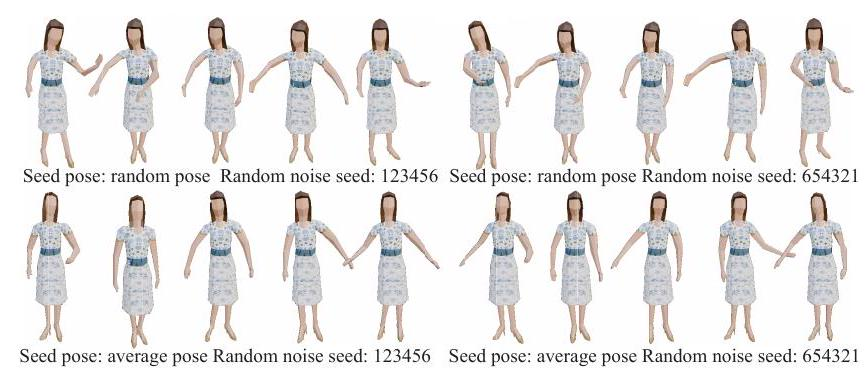
\includegraphics[width=\linewidth]{images/random_gesture_result.jpg}
%     \caption[Sự đa dạng của các cử chỉ]{Sự đa dạng của các cử chỉ. Mọi người thực hiện các cử chỉ đồng thoại khác nhau ở những thời điểm khác nhau trong các trạng thái khác nhau. Giống như con người thực tế, đối với cùng một bài nói, phương pháp của chúng tôi có khả năng tạo ra các cử chỉ khác nhau với hạt gieo khác nhau hoặc với cử chỉ nhiễu khác nhau}
%     \label{fig:randomgestureresult}
% \end{figure}


% \begin{center}
% \begin{tabular}{lcc}
% \hline
% \multicolumn{1}{c}{Tên} & \begin{tabular}{c}
% Con người $_{\text {tương đồng }} \uparrow$ \
% giống \
% \end{tabular} & \begin{tabular}{c}
% Phù hợp \
% ngôn ngữ - cử chỉ \
% \end{tabular} \
% \hline
% Sự thật & $4.15 \pm 0.11$ & $4.25 \pm 0.09$ \
% Chúng tôi & $\mathbf{4 . 1 1} \pm \mathbf{0 . 0 8}$ & $\mathbf{4 . 1 1} \pm \mathbf{0 . 1 0}$ \

% WavLM & $4.05 \pm 0.10$ & $3.91 \pm 0.11$ \
% tập trung chéo cục bộ & $3.76 \pm 0.09$ & $3.51 \pm 0.15$ \
% tập trung tự & $3.55 \pm 0.13$ & $3.08 \pm 0.10$ \
% chú ý + GRU & $3.10 \pm 0.11$ & $2.98 \pm 0.14$ \
% tập trung xuôi & $3.75 \pm 0.15$ & $3.23 \pm 0.24$ \
% \hline
% \end{tabular}
% \end{center}


% % Bảng 1: Kết quả nghiên cứu rút gọn. '-' chỉ ra các mô-đun không được sử dụng và ' + ' chỉ ra các mô-đun bổ sung. Chữ đậm chỉ ra số liệu tốt nhất.

% Do kiến trúc mô hình của chúng tôi, thậm chí đối với cùng một bài nói và phong cách, các cử chỉ nhiễu khác nhau và các hạt gieo khác nhau có thể tạo ra kết quả khác nhau, như thể hiện trong \autoref{fig:randomgestureresult}. Điều này giống như bài nói thực của con người, tạo ra các cử chỉ đồng thoại đa dạng liên quan đến vị trí ban đầu. Phân tích của chúng tôi trước đó được thực hiện trên chiều phong cách. Lưu ý rằng mô hình cũng thêm một mặt nạ ngẫu nhiên vào xử lý của hạt gieo, vì vậy nó cũng có thể nội suy và mở rộng các hạt gieo khác nhau để kiểm soát việc tạo ra cử chỉ với vị trí ban đầu khác nhau và đa dạng.

% \begin{table}[h]
% \caption{Đánh giá độ tương đồng và phù hợp ngôn ngữ-cử chỉ của các mô hình}
% \label{tab:evaluation}
% \begin{tabularx}{\textwidth}{l*{2}{>{\centering\arraybackslash}X}}
% \toprule
% \textbf{Tên} & \textbf{Con người (Tương đồng)} & \textbf{Phù hợp ngôn ngữ-cử chỉ} \\
% \midrule
% Sự thật & $4.15 \pm 0.11$ & $4.25 \pm 0.09$ \\
% Chúng tôi & $\mathbf{4.11 \pm 0.08}$ & $\mathbf{4.11 \pm 0.10}$ \\
% WavLM & $4.05 \pm 0.10$ & $3.91 \pm 0.11$ \\
% Tập trung chéo cục bộ & $3.76 \pm 0.09$ & $3.51 \pm 0.15$ \\
% Tập trung tự & $3.55 \pm 0.13$ & $3.08 \pm 0.10$ \\
% Chú ý + GRU & $3.10 \pm 0.11$ & $2.98 \pm 0.14$ \\
% Tập trung xuôi & $3.75 \pm 0.15$ & $3.23 \pm 0.24$ \\
% \bottomrule
% \end{tabularx}
% \end{table}

% \caption{Kết quả nghiên cứu rút gọn. '-' chỉ ra các mô-đun không được sử dụng và ' + ' chỉ ra các mô-đun bổ sung. Chữ đậm chỉ ra số liệu tốt nhất.}

% \section{Các thông tin thực nghiệm bổ sung}

% Hơn nữa, chúng tôi thực hiện nghiên cứu giảm thiểu để đánh giá ảnh hưởng hiệu suất của các thành phần khác nhau trong mô hình của chúng tôi. Vì phù hợp giữa cử chỉ và phong cách có thể được kiểm soát bằng tham số và ảnh hưởng đến hai chiều còn lại, chúng tôi đặt $\gamma$ là 1 và chỉ đánh giá sự giống nhân văn và phù hợp giọng nói để dễ so sánh. Kết quả của nghiên cứu giảm thiểu của chúng tôi được tóm tắt trong Bảng 1. Các so sánh hình ảnh của nghiên cứu này cũng có thể được tham khảo trong video bổ sung. Chúng tôi khám phá độ hiệu quả của các thành phần sau đây:
% (1) features WavLM 
% (2) local attention
% (3) local attention pattern
% (4) self-attention
% (5) attention
% Chúng tôi tiến hành thực nghiệm trên từng thành phần trong năm thành phần này, mỗi thành phần một lần.

% \subsection{Nghiên Cứu Người Dùng}
% Được hỗ trợ bởi kết quả trong Bảng 1, khi chúng tôi không sử dụng đặc trưng WavLM mà thay vào đó sử dụng 13 hệ số đầu tiên của hệ số cepstral tần số Mel (MFCC), điểm số của cả hai chiều đều giảm, đặc biệt là phù hợp giọng nói. Điều này là do các đặc trưng được trích xuất bởi mô hình WavLM đã được huấn luyện trước chứa nhiều thông tin như ngữ nghĩa và cảm xúc, giúp tạo ra các cử chỉ tương ứng. Khi không có sự chú ý cục bộ chéo, điểm số của cả hai chiều giảm rất nhiều. Bởi vì nhiều bước tạo ra cử chỉ chỉ liên quan đến các tương quan trong phạm vi ngắn, chú ý cục bộ có thể nắm bắt thông tin cục bộ tốt hơn, điều này khớp với quan sát của \cite{rae2020transformers}. Chỉ có chú ý tự dựa vào thông tin toàn cầu của các dãy dài trở nên ít hiệu quả hơn. 
% Cả giống nhân văn và sự phù hợp giữa cử chỉ và giọng nói giảm nhiều hơn khi chúng ta loại bỏ chú ý tự, ngụ ý rằng chú ý tự quan trọng hơn chú ý cục bộ vì có sự không đồng bộ tích cực giữa giọng nói và cử chỉ, và khó khăn để học đủ thông tin cử chỉ từ chỉ một cửa sổ cục bộ (gần như nửa giây) của giọng nói.
% Khi không sử dụng chú ý, chúng tôi thay thế nó bằng một mô hình dựa trên GRU, có kết quả tồi tệ nhất trong tất cả các mô hình, làm rõ thêm hiệu suất của cơ chế chú ý. 
% Ngoài ra, chúng tôi thực nghiệm sử dụng cấu trúc chú ý trong \autoref{fig:type_attention} và thấy rằng hiệu ứng trở nên tồi tệ hơn. Sự khác biệt duy nhất giữa việc thêm chú ý chuyển tiếp và chú ý cục bộ sử dụng trong mô hình của chúng tôi là cử chỉ được tạo ra với việc nhìn thêm vào thông tin giọng nói trong một cửa sổ tương lai. Điều này là một phát hiện thú vị, mặc dù có sự không đồng bộ ngầm giữa giọng nói và cử chỉ, theo một số cách, nó có thể chỉ ra rằng cử chỉ có liên quan hơn đến một khoảng thời gian ngắn trong hiện tại và quá khứ và không phải là một khoảng thời gian ngắn trong tương lai. Nó cũng có thể có khả năng rằng những người khác nhau có các phong cách khác nhau và tập dữ liệu này chỉ có một diễn viên cần được nghiên cứu thêm.

% % \section{Tập dữ liệu}

% % Bảng dữ liệu được chúng tôi trình bày dưới đây

% % \begin{adjustbox}{max width=\textwidth}
% % \begin{table}[htbp]
% %     \centering
% %     \begin{tabular}{|l|l|l|l|}
% %         \hline
% %         \textbf{Dataset} & \textbf{Modalities} & \textbf{Type} & \textbf{Download} \\
% %         \hline
% %         IEMOCAP & gesture_motion, audio, text, emotion & dialog & \href{https://sail.usc.edu/iemocap}{sail.usc.edu/iemocap} \\
% %         & & & \href{https://arxiv.org/pdf/1810.12541.pdf}{[paper]} \\
% %         \hline
% %         Creative-IT & gesture_motion, audio, text, emotion & dialog & \href{https://sail.usc.edu/CreativeIT/ImprovRelease.htm}{sail.usc.edu/CreativeIT} \\
% %         \hline
% %         Gesture-Speech Dataset & gesture_motion, audio & monolog & \href{https://www.dropbox.com/sh/j419kp4m8hkt9nd/AAC_pIcS1b_WFBqUp5ofBG1Ia?dl=0}{dropbox} \\
% %         \hline
% %         CMU Panoptic & gesture_motion, audio, text & dialog & \href{http://domedb.perception.cs.cmu.edu}{domedb.perception.cmu} \\
% %         & & & \href{https://arxiv.org/abs/1612.03153}{[paper]} \\
% %         \hline
% %         Speech-Gesture & gesture_motion, audio & monolog & \href{https://github.com/amirbar/speech2gesture}{amirbar/speech2gesture} \\
% %         & & & \href{https://arxiv.org/abs/1906.04160}{[paper]} \\
% %         \hline
% %         TED Dataset & gesture_motion, audio & monolog & \href{https://github.com/youngwoo-yoon/youtube-gesture-dataset}{youtube-gesture-dataset} \\
% %         & & & \href{https://sites.google.com/view/youngwoo-yoon/projects/co-speech-gesture-generation}{[homepage]} \\
% %         \hline
% %         Talking With Hands & gesture_motion, audio & dialog & \href{https://github.com/facebookresearch/TalkingWithHands32M}{facebookresearch/TalkingWithHands32M} \\
% %         & & & \href{https://personalrobotics.cs.washington.edu/publications/lee2019handmotiondataset.pdf}{[paper]} \\
% %         \hline
% %         PATS & gesture_motion, audio, text & monolog & \href{https://chahuja.com/pats}{chahuja.com/pats} \\
% %         & & & \href{https://arxiv.org/pdf/2007.12553v1.pdf}{[paper]} \\
% %         \hline
% %         Trinity Speech-Gesture I & gesture_motion, audio, text & monolog & \href{https://trinityspeechgesture.scss.tcd.ie/data/Trinity%20Speech-Gesture%20I/GENEA_Challenge_2020_data_release}{Trinity Speech-Gesture I} \\
% %         \hline
% %         Trinity Speech-Gesture II & gesture_motion, audio, segment & monolog & \href{https://trinityspeechgesture.scss.tcd.ie/data/Trinity%20Speech-Gesture%20II}{Trinity Speech-Gesture II} \\
% %         \hline
% %         Speech-Gesture 3D extension & gesture_motion, audio & monolog & \href{https://nextcloud.mpi-klsb.mpg.de/index.php/s/7LzxGSepzrndg2x}{nextcloud.mpi-klsb} \\
% %         \hline
% %         Talking With Hands GENEA Extension & gesture_motion, audio, text & dialog & \href{https://zenodo.org/record/6998231}{zenodo/6998231} \\
% %         & & & \href{https://dl.acm.org/doi/abs/10.1145/3536221.3558068}{[paper]} \\
% %         \hline
% %         SaGA & gesture_motion, audio, properties & dialog & \href{https://www.phonetik.uni-muenchen.de/Bas/BasSaGAeng.html}{phonetik.uni-muenchen} \\
% %         & & & \href{https://pub.uni-bielefeld.de/record/2001935}{[paper]} \\
% %         \hline
% %         SaGA++ & gesture_motion, audio, properties & dialog & \href{https://zenodo.org/record/6546229}{zenodo/6546229} \\
% %         \hline
% %         ZEGGS Dataset & gesture_motion, audio & monolog & \href{https://github.com/ubisoft/ubisoft-laforge-ZeroEGGS}{ubisoft-laforge-ZeroEGGS} \\
% %         & & & \href{https://arxiv.org/abs/2209.07556}{[paper]} \\
% %         \hline
% %         BEAT Dataset & gesture_motion, audio, text, properties, emotion & dialog, monolog & \href{https://pantomatrix.github.io/BEAT}{github.io/BEAT} \\
% %         & & & \href{https://arxiv.org/pdf/2203.05297.pdf}{[paper]} \\
% %         \hline
% %     \end{tabular}
% % \end{table}
% % \end{adjustbox}
% % % \caption{List of Datasets in Speech and Gesture Domain}
% % \label{tab:datasets}

%\section{Kết quả minh hoạ sau quá trình render}
%
%\begin{quote}
%	{
%		"Your work is gonna fill a large part of your life . And the only way to be truly satisfied is to do what you believe is great work and the only way to do great work is to love what you do."}
%\end{quote}
%
%\begin{figure}[h]
%	\centering
%	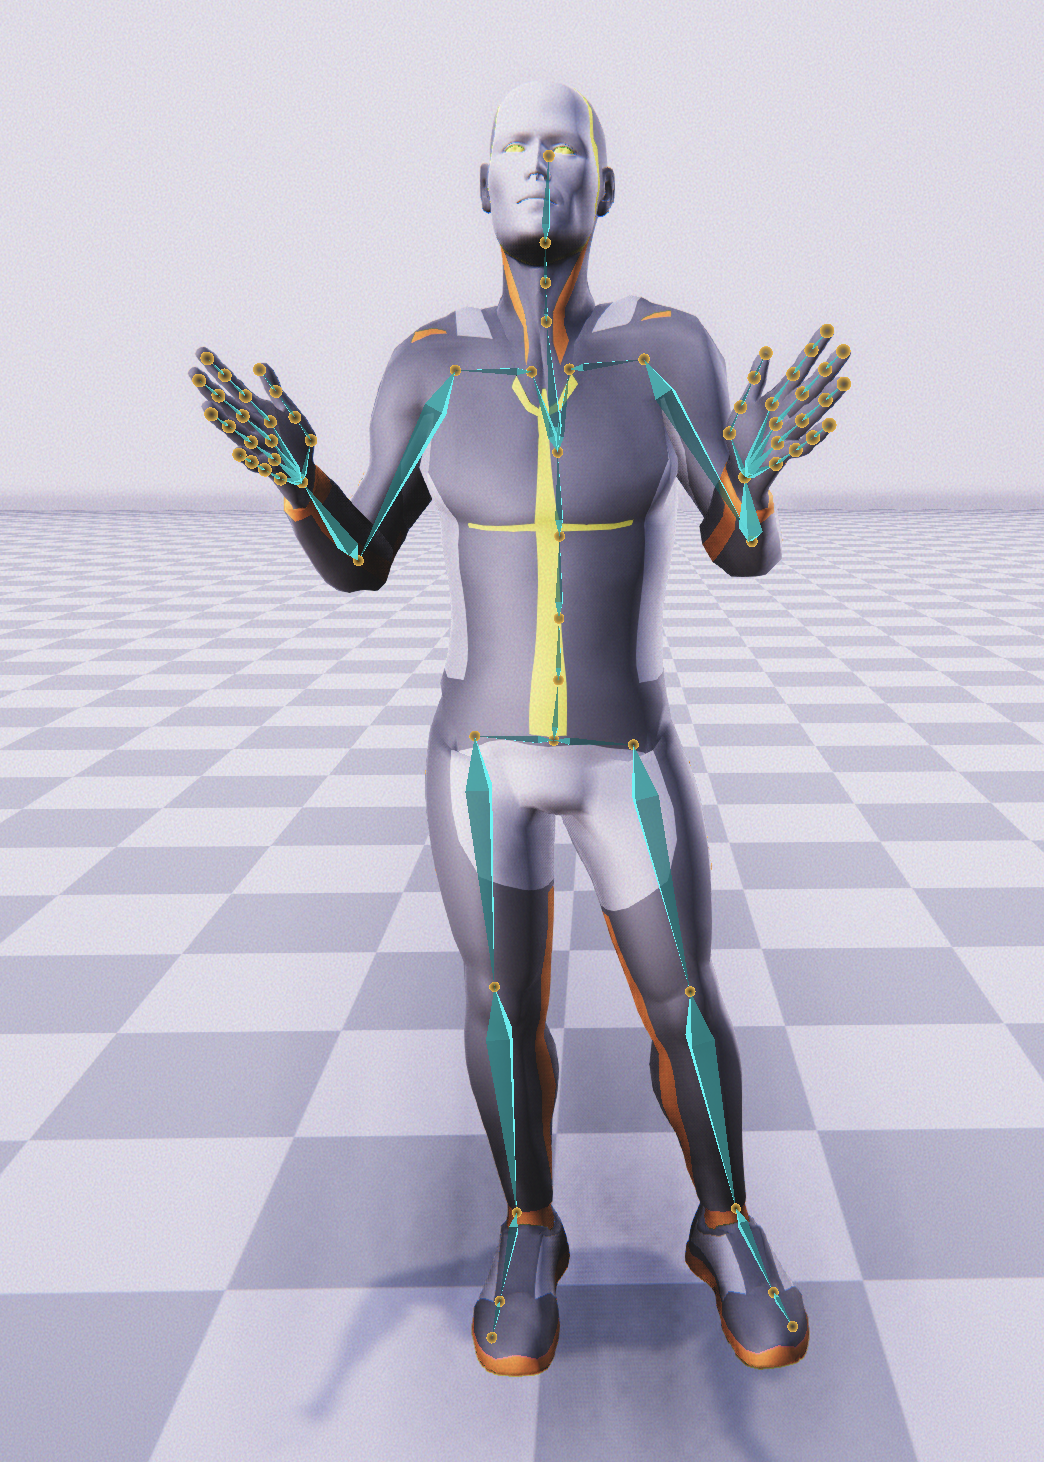
\includegraphics[height={6cm}]{SampleAnimation}
%	
%	\caption{Steven Job - Speech-Driven Gesture Generation}
%	\label{fig:SampleAnimation}
%
%\end{figure}
%
%\href{https://www.youtube.com/watch?v=B6nv1kQmi-Q}{\textcolor{blue}{\uline{youtube.com/watch?v=B6nv1kQmi-Q}}}


%
%\chapter{KẾT LUẬN VÀ KIẾN NGHỊ}
\label{Chapter5}

\section{Kết quả đạt được}

%Trong luận văn này, mô hình sinh cử chỉ của chúng tôi đã có kết quả sinh cử rất giống người, và hệ thống không chỉ có khả năng sinh cử chỉ đồng bộ với cảm xúc và nội dung của âm thanh đầu vào mà còn có thể suy luận dữ liệu không có trong tập huấn luyện. Ngoài ra, chúng tôi cũng đóng góp mô hình pretrain trên Huggingface (\hyperlink{https://huggingface.co/openhuman/openhuman}{huggingface.co/openhuman/openhuman}) và toàn bộ mã nguồn chương trình OHGesture ở github công khai \hyperlink{https://github.com/hmthanh/OHGesture}{hmthanh/OHGesture}.
%Chúng tôi cũng upload toàn bộ các video render của mô hình lên Youtube để có thể so sánh kết quả giữa các mô hình, cũng như kết quả minh hoạ của mô hình OHGesture và GroundTruth.
%
%Chúng tôi mở rộng dữ liệu đầu vào không chỉ bao gồm cử chỉ, âm thanh và nhãn cảm xúc. Mà còn sử dụng các công cụ chuyển văn bản thành giọng nói để transcribe âm thanh thành văn bản. Từ đó có thêm nguồn dữ liệu cho quá trình học khử nhiễu có điều kiện.
%
%Tuy nhiên, do hạn chế tài nguyên, các đánh giá hiện tại vẫn chủ yếu dựa trên các kết quả chủ quan và kết quả từ mô hình cơ sở, chưa hoàn toàn phản ánh chất lượng thực tế của hệ thống đề xuất.

Trong luận văn này, chúng tôi đã phát triển và thử nghiệm thành công mô hình sinh cử chỉ OHGesture, một hệ thống có khả năng tạo ra cử chỉ rất tự nhiên, mang lại cảm giác giống người. Điểm nổi bật của mô hình là khả năng đồng bộ chính xác giữa cử chỉ và cảm xúc, nội dung của âm thanh đầu vào, đồng thời có khả năng suy luận vượt ra khỏi các dữ liệu được huấn luyện ban đầu. Điều này có nghĩa là mô hình dựa trên Diffusion  không chỉ phụ thuộc vào các mẫu dữ liệu cử chỉ đã được học mà còn có thể có tính khái quát hoá cao, và có thể sinh cử chỉ cho các âm thanh và ngữ cảnh có xác xuất dữ liệu thấp.

%Để hỗ trợ cộng đồng nghiên cứu và mở rộng ứng dụng, chúng tôi đã cung cấp phiên bản pretrained của mô hình OHGesture trên nền tảng Huggingface, có thể truy cập tại địa chỉ \hyperlink{https://huggingface.co/openhuman/openhuman}{huggingface.co/openhuman/openhuman}. Bên cạnh đó, toàn bộ mã nguồn của mô hình cùng các cải tiến trong quá trình xử lý dữ liệu và sinh cử chỉ đã được công khai trên GitHub tại kho lưu trữ \hyperlink{https://github.com/hmthanh/OHGesture}{hmthanh/OHGesture}, cho phép các nhà nghiên cứu và nhà phát triển dễ dàng tải xuống, tùy chỉnh và thử nghiệm. Để hỗ trợ việc đánh giá và so sánh kết quả, chúng tôi cũng đã tải lên toàn bộ các video render của mô hình trên YouTube, giúp trực quan hóa và đối chiếu giữa kết quả cử chỉ sinh ra bởi OHGesture và cử chỉ từ dữ liệu thực tế (GroundTruth).

Một điểm đáng chú ý khác trong nghiên cứu này là việc mở rộng dữ liệu đầu vào. Chúng tôi không chỉ giới hạn ở cử chỉ, âm thanh và nhãn cảm xúc mà còn tích hợp thêm các công cụ chuyển đổi văn bản thành giọng nói để chuyển âm thanh thành văn bản. Nhờ vậy, mô hình có thêm nguồn thông tin để học cách khử nhiễu có điều kiện, giúp hệ thống hiểu rõ hơn ngữ cảnh và tạo ra cử chỉ phù hợp với từng nội dung cụ thể.

%Tuy nhiên, do hạn chế về tài nguyên, việc đánh giá chất lượng của mô hình hiện tại vẫn chủ yếu dựa trên các kết quả chủ quan và kết quả của các mô hình cơ sở. Dù cho các kết quả đánh giá này khá khả quan, chúng chưa thể hoàn toàn phản ánh chất lượng thực tế của hệ thống đề xuất trong mọi bối cảnh và điều kiện. Điều này là một hạn chế cần được cải thiện trong các nghiên cứu tiếp theo nhằm đạt được sự đánh giá chính xác và toàn diện hơn.



\section{Ưu và nhược điểm của mô hình}


Mô hình sinh cử chỉ OHGesture có nhiều ưu điểm đáng kể, góp phần quan trọng trong việc phát triển các hệ thống tương tác người-máy tự nhiên và linh hoạt hơn. Tuy nhiên, vẫn còn một số nhược điểm để cải thiện hiệu quả trong tương lai.

\textbf{Ưu điểm:}

\begin{itemize}
	\item Độ chân thực cao: Dựa vào kết quả sinh cử chỉ, có thể thấy mô hình OHGesture đã đạt được kết quả sinh cử chỉ có độ giống người cao. Các cử chỉ sinh ra phản ánh được sắc thái và nhịp điệu của âm thanh, giúp hệ thống có khả năng phản hồi đồng bộ với thông tin cảm xúc và nội dung của lời nói.
	
	\item Khả năng tổng quát tốt: Nhờ mô hình khử nhiễu có thể phủ được các điểm dữ liệu có các xác xuất thấp, mô hình có thể suy luận cử chỉ cho các tình huống và trạng thái cảm xúc chưa từng xuất hiện trong tập huấn luyện, cho thấy tiềm năng ứng dụng trong nhiều bối cảnh thực tế.
	
	\item Có khả năng kiểm soát được nhiều đặc trưng khác nhau: Mô hình diffusion có khả năng điều khiển được các cảm xúc khác nhau, có khả năng nội suy trạng thái giữa các cảm xúc khác nhau.
	
%	\item 
	
%	Dễ dàng triển khai và mở rộng: Việc công khai mã nguồn và mô hình pretrain trên Huggingface giúp cộng đồng dễ dàng tiếp cận, triển khai và mở rộng mô hình. Điều này tạo điều kiện cho các nhà nghiên cứu và nhà phát triển khác đóng góp, cải tiến mô hình một cách nhanh chóng và hiệu quả.
	
	\end{itemize}



\textbf{Nhược điểm:}

\begin{itemize}
	\item Mô hình hiện chưa có khả năng sampling theo thời gian thực (real time) và cần nhiều bước để ra kết quả cuối cùng.
	
	\item Thông tin đặc trưng theo $D=1141$ được xử lý như một tấm ảnh, không thể hiện đúng đặc trưng chuyển động.
	
	\item Phụ thuộc vào dữ liệu đầu vào chất lượng cao: Mô hình yêu cầu dữ liệu âm thanh đầu vào có chất lượng tốt và rõ ràng để đảm bảo độ chính xác của cử chỉ sinh ra. Khi âm thanh đầu vào bị nhiễu hoặc chứa nhiều biến thể cảm xúc khó phân biệt, độ chính xác của cử chỉ sinh ra có thể giảm sút.
	
%	\item 
%	Thiếu các tiêu chuẩn đánh giá khách quan: Hiện nay, các đánh giá về chất lượng cử chỉ sinh ra vẫn dựa nhiều vào ý kiến chủ quan của người dùng, khiến việc so sánh chính xác giữa các mô hình khác nhau gặp khó khăn. Việc thiếu các phương pháp đánh giá tự động, đáng tin cậy làm hạn chế khả năng cải tiến liên tục của mô hình.
	
%	\item Yêu cầu tài nguyên tính toán lớn: Mô hình cần tài nguyên tính toán cao, như GPU mạnh, để có thể huấn luyện và suy luận hiệu quả, điều này có thể là rào cản cho các ứng dụng thực tế trên thiết bị có cấu hình thấp hoặc trong môi trường tính toán giới hạn.
	
	
\end{itemize}


%\section{Hạn chế và hướng phát triển}
%
%Mặc dù hệ thống sinh cử chỉ của chúng tôi đã đạt được những kết quả khả quan, vẫn còn một số hạn chế cần khắc phục. Đầu tiên, chất lượng sinh cử chỉ có thể bị ảnh hưởng bởi tính phức tạp của âm thanh đầu vào, đặc biệt khi âm thanh chứa nhiều yếu tố gây nhiễu hoặc cảm xúc chưa được biểu đạt rõ ràng. Bên cạnh đó, việc đánh giá chất lượng mô hình vẫn chủ yếu dựa trên đánh giá chủ quan của con người, dẫn đến khả năng thiếu nhất quán và khó khăn trong việc so sánh chính xác với các mô hình hiện có.
%
%Trong tương lai, hướng phát triển tiếp theo sẽ tập trung vào việc tối ưu hóa mô hình để cải thiện độ chính xác và tính ổn định của cử chỉ sinh ra trong các tình huống phức tạp. Đồng thời, việc mở rộng dữ liệu huấn luyện để bao quát thêm nhiều trạng thái cảm xúc và bối cảnh khác nhau có thể giúp mô hình đáp ứng tốt hơn các tình huống đa dạng. Chúng tôi cũng đề xuất nghiên cứu thêm các phương pháp đánh giá tự động, nhằm giảm thiểu sự phụ thuộc vào các đánh giá chủ quan. Bên cạnh đó, tích hợp các công cụ trí tuệ nhân tạo khác, như mô hình hiểu ngữ cảnh và phân tích cảm xúc, sẽ là bước tiến quan trọng để nâng cao tính linh hoạt và độ chính xác của hệ thống trong việc hiểu và sinh động các cử chỉ đồng bộ với nội dung và cảm xúc của lời nói.

\section{Phương hướng phát triển và nghiên cứu trong tương lai}


Trong tương lai, có nhiều hướng phát triển tiềm năng để cải thiện và mở rộng mô hình sinh cử chỉ OHGesture, nhằm đáp ứng tốt hơn các yêu cầu thực tế và nâng cao tính ứng dụng của hệ thống. Một số hướng nghiên cứu và phát triển chính bao gồm:

\begin{itemize}
	\item Tối ưu hoá mô hình để có thể chay theo thời gian thực, hiện tại mô hình phải chia chuỗi âm thanh, và kết quả sinh phải được  import vào Unity mới có thể render. Trong tương lai, chúng tôi mong muốn có thể xây dựng các hệ thống với thời gian thực. để có thể tương tác và tăng tính ứng dụng của mô hình
	
	\item Tối ưu hóa quá trình sampling và giảm số bước lấy mẫu: Hiện tại, quá trình sinh cử chỉ đòi hỏi một số bước lấy mẫu (sampling steps) tương đối lớn, ảnh hưởng đến tốc độ và hiệu quả của hệ thống. Việc tối ưu hóa để giảm số bước sampling mà không làm suy giảm chất lượng cử chỉ sinh ra sẽ giúp mô hình đáp ứng nhanh hơn và phù hợp cho các ứng dụng thời gian thực.
	
	\item Tích hợp và thử nghiệm các kỹ thuật embedding mới: Sử dụng các phương pháp embedding mới, đa dạng hóa thông tin đầu vào có thể giúp mô hình hiểu và phản ánh tốt hơn ngữ cảnh và cảm xúc của giọng nói. Đây cũng là một hướng phát triển để nâng cao khả năng của hệ thống trong việc sinh cử chỉ phù hợp với ngữ nghĩa của các ngôn ngữ khác nhau.
	
	\item Mở rộng sang đa ngôn ngữ và đa văn hóa: Hiện tại, mô hình chủ yếu hoạt động với các dữ liệu âm thanh tiếng Anh. Nghiên cứu mở rộng mô hình để sinh cử chỉ cho các ngôn ngữ và nền văn hóa khác nhau sẽ là một bước tiến quan trọng, giúp hệ thống trở nên đa dạng và ứng dụng rộng rãi hơn.
	
	\item Kết hợp với mô hình DeepPhase \cite{starke2022deepphase} để đạt hiệu quả sinh cử chỉ thời gian thực: Mục tiêu của chúng tôi là tích hợp OHGesture với mô hình DeepPhase để phát triển hệ thống có khả năng phản hồi cử chỉ trong thời gian thực, ứng dụng trong các tình huống giao tiếp tự nhiên như hội thoại người-máy và các hệ thống điều khiển bằng giọng nói. Với mục tiêu là sẽ học các đặc trưng về pha của các chuyển động để có thể trích xuất được các đặc trưng chuyển động, thay vì sử dụng đặc trưng như một tấm ảnh của mô hình.
	
%	\item Trong tương lai, 
	
	\item Cải thiện đánh giá khách quan bằng các độ đo tự động: Để giảm sự phụ thuộc vào các đánh giá chủ quan, cần phát triển và tích hợp các phương pháp đánh giá tự động đáng tin cậy, cho phép mô hình có thể tự đánh giá và điều chỉnh theo các chỉ số khách quan.
	\end{itemize}



\section{Đóng góp của luận văn}

Trong luận văn này, chúng tôi đã phát triển hệ thống sinh cử chỉ OHGesture, với các đóng góp quan trọng như sau:

\begin{itemize}
	\item Phát triển mô hình sinh cử chỉ dựa trên Diffusion: Hệ thống OHGesture được thiết kế để tạo ra các cử chỉ đồng bộ với âm thanh đầu vào và phản ánh đúng cảm xúc. Mô hình này còn có khả năng tổng quát hoá, cho phép sinh cử chỉ ngay cả với các mẫu âm thanh ngoài dữ liệu huấn luyện, mang lại độ chân thực cao.
	
	\item Công khai mã nguồn và mô hình trên các nền tảng mở: Để thúc đẩy ứng dụng và cải tiến từ cộng đồng, chúng tôi đã cung cấp mã nguồn trên GitHub, chúng tôi mở rộng mã nguồn, và được công khai ở \hyperlink{https://github.com/hmthanh/OHGesture}{hmthanh/OHGesture} và một phiên bản pretrained trên Huggingface \hyperlink{https://huggingface.co/openhuman/openhuman}{huggingface.co/openhuman/openhuman}, giúp các nhà nghiên cứu khác dễ dàng tiếp cận, tái hiện và mở rộng hệ thống.
	
	\item Tích hợp thêm văn bản và âm thanh chuyển ngữ trong quá trình sinh cử chỉ: Với tập dữ liệu ZeroEGGS chỉ bao gồm âm thanh, cử chỉ và nhãn cảm xúc, chúng tôi sử dụng các API của Azure và Google để transcribe các tệp âm thanh thành văn bản. Giúp mở rộng dữ liệu đầu vào của mô hình sinh cử chỉ thêm đặc trưng văn bản, giúp hệ thống có thêm ngữ cảnh để sinh ra các cử chỉ phù hợp hơn với nội dung cụ thể.
	
	\item Đóng góp vào việc xây dựng hệ thống đánh giá chuẩn hóa: Chúng tôi đang phát triển một hệ thống xếp hạng trực tuyến \hyperlink{https://genea-workshop.github.io/leaderboard/}{GENEA Leaderboard} \cite{nagy2024towards} cho các mô hình sinh cử chỉ. Chúng tôi đã thu thập và xử lý các dữ liệu cử chỉ từ nhiều nguồn ngôn ngữ và tập dữ liệu khác nhau, tạo thành một tập dữ liệu chuẩn hóa duy nhất. Xây dựng một bản xếp hạng để so sánh nhiều mô hình khác nhau. Và sử dụng người để đánh giá các mô hình sinh, giúp đánh giá chính xác kết quả sinh của cử chỉ so với các độ đo trước đây, vốn không thể đo được sự phức tạp và đa dạng trong chuyển động của cử chỉ tương ứng với âm thanh. Điều này giúp tạo nên một nền tảng dữ liệu thống nhất, hỗ trợ việc đánh giá đồng nhất giữa các mô hình. Từ đó thúc đẩy tính thống nhất trong lĩnh vực sinh cử chỉ trong cộng đồng nghiên cứu.
	
	\item Xây dựng công cụ trực quan hoá bằng Unity: Các hệ thống trực quan hoá cử chỉ hiện nay đề dự trên Blender, và không đạt kết quả hiển thị tốt khi sinh cử chỉ, bằng việc kết thừa mã nguồn từ mô hình \cite{starke2022deepphase}, chúng tôi đã tạo ra một hệ thống trực quan hoá quá sinh sinh cử chỉ và so sánh giữa các mô hình. 
	
	\item Xây dựng hướng phát triển trong tương lai: Dựa trên nền tảng của mô hình diffusion và hiểu rõ bản chất của quá trình sinh cử chỉ, chúng tôi có thể kết hợp các mô hình sinh cử chỉ dựa trên pha với các thuật toán xử lý và trích xuất thông tin, nhằm tối ưu hóa chất lượng và tính phù hợp của các cử chỉ được sinh ra. Hướng phát triển này mở ra triển vọng cho các cải tiến sâu rộng trong việc tương tác giữa cử chỉ và các yếu tố ngữ cảnh phức tạp như biểu cảm khuôn mặt, ngữ điệu và động lực cảm xúc, tạo nền tảng cho những bước tiến trong các ứng dụng giao tiếp người - máy và các lĩnh vực liên quan khác.
\end{itemize}








\section{Lời kết}
%\ref{fig:SampleAnimation}
%Qua kết quả sinh cử chỉ thực tế sau khi render, có thể thấy mô hình của chúng tôi kế thừa từ mô hình DiffuseStyleGesture đạt kết quả tốt khi kết xuất, không chỉ có thể sinh ra cử chỉ chân thật từ dữ liệu GroundTruth mà còn có thể suy luận ra những cử chỉ không hề có trong tập dữ liệu huấn luyện như âm thanh của Steven Jobs nói. Điều này cũng chứng tỏ rằng mô hình Diffusion là mô hình có thể đạt kết quả tốt để có thể phủ được các kết quả sinh mà ở đó xác xuất dữ liệu thấp. Ngoài đóng góp về việc tích hợp thêm văn bản vào quá trình sinh cử chỉ, mã nguồn chỉnh sửa được công khai trên Github, chúng tôi cũng đóng góp về quá trình kết xuất và quá trình xử lý dữ liệu trên Unity. Đây là nền tảng để tiếp tục nghiên cứu và cải thiện mô hình OHGesture hiện tại.

%Việc học cử chỉ tương ứng với giọng nói (speech-drive gesture generation) không chỉ đạt kết quả tốt với dữ liệu gốc mà cử chỉ còn có thể sinh ra cử chỉ đạt kết quả tốt ở những âm thanh không có trong dữ liệu như 


%Trong tương lai, vẫn còn nhiều bước có thể cải tiến, như giảm số bước sampling, tối ưu các tham số và sử dụng các embedding mới, cũng như sinh cử chỉ cho các văn bản của ngôn ngữ khác. Mục tiêu của chúng tôi là tích hợp với mô hình \hyperlink{https://deepgesture.github.io/}{DeepGesture} để có thể sinh cử chỉ theo thời gian thực.




Qua quá trình thử nghiệm và phân tích kết quả sinh cử chỉ thực tế, mô hình OHGesture của chúng tôi đã kế thừa và phát triển từ mô hình DiffuseStyleGesture, có khả năng sinh cử chỉ chân thực, không chỉ trên các mẫu dữ liệu trong tập huấn luyện mà còn mở rộng được với những âm thanh không có trong dữ liệu huấn luyện, ví dụ như giọng nói của Steven Jobs. Điều này minh chứng cho tiềm năng của mô hình Diffusion trong việc sinh cử chỉ cho các dữ liệu hiếm, nơi xác suất dữ liệu thấp.

Bên cạnh đó, chúng tôi đã đóng góp các mã nguồn chỉnh sửa trên Github, bao gồm quá trình kết xuất và xử lý dữ liệu trên nền tảng Unity, tạo nền tảng thuận lợi cho các nghiên cứu và cải tiến tiếp theo đối với mô hình OHGesture. Việc kết hợp thêm văn bản vào quá trình sinh cử chỉ cũng là một bước đột phá, mở ra nhiều hướng phát triển ứng dụng trong các lĩnh vực yêu cầu tương tác tự nhiên và hiệu quả hơn.

%Qua quá trình thực nghiệm, chúng tôi có thể chứng mô hình \textbf{OHGesture} đạt được kết quả sau:

%1). Mô hình đạt kết quả tốt trong việc sinh cử chỉ dựa trên âm thanh, tạo ra các cử chỉ chất lượng cao, giống con người (human-likeness).
%
%2) Dựa trên phương pháp Classifier-Free Guidance, chúng tôi có thể sử dụng mô hình diffusion có điều kiện, với điều kiện bao gồm cảm xúc và cử chỉ khởi tạo. Mô hình đã có thể nội suy ra được những cảm xúc, hoặc khoảng cách ở giữa hai cảm xúc. 
%
%3) Dựa vào cơ chế self-attention và cross attention, chúng tôi có thể sinh ra cử chỉ tương ứng với giọng nói, có khả năng liên với bối cảnh.

%Mô hình của chúng tôi tổng hợp các cử chỉ sao cho chúng khớp với nhịp âm thanh và ngữ nghĩa văn bản dựa trên các cơ chế tập trung chéo và tập trung tự.

%3) Sử dụng phương pháp huấn luyện hướng dẫn không cần bộ phân loại, chúng ta có thể kiểm soát các điều kiện cụ thể, tức là cảm xúc và cử chỉ khởi tạo, và thực hiện nội suy hoặc mở rộng để đạt được một mức kiểm soát cao đối với các cử chỉ được tạo ra.

%4) Kết quả thực nghiệm cho thấy, mô hình của chúng tôi có thể sinh cử chỉ đạt kết quả tốt ngay cả với trường hợp âm thanh không nằm trong tập huấn luyện.
%
%Trong các độ đo về human-likeness, emotion-likeness và speech appropriateness mô hình của chúng tôi vượt trội so với các phương pháp hiện có trong nhiệm vụ tạo ra cử chỉ đồng thời dựa trên âm thanh và thể hiện khả năng thao tác phong cách cao hơn.
%Trong hướng nghiên cứu tương lai, chúng tôi dự định sẽ sử dụng các thuật toán Fourier để tách chuỗi chuyển động của cử chỉ để có thể học được pha trong các chuyển động cử chỉ.
% Còn nhiều không gian để cải thiện trong nghiên cứu này, ví dụ, giải quyết vấn đề nhiều bước lấy mẫu và tiêu thụ thời gian lâu của các phương pháp diffusion để sử dụng trong các hệ thống thời gian thực là hướng nghiên cứu của chúng tôi trong tương lai.

% Trong phần này chúng tôi đưa ra các kết quả đạt được của mô hình chúng tôi, chúng tôi cố gắng tìm hiểu các đặc trưng của các bộ dữ liệu tương ứng để cố gắng lý giải thích tại sao mô hình của chúng tôi hoặc các công trình khác có được kết quả tốt trên tập dữ liệu tương ứng đó. Những kết quả của hai đề xuất của chúng tôi cũng như các dịnh hướng nghiên cứu của chúng tôi trong tương lai.

% Mặc dù kết quả chúng tôi cho thấy phương pháp của chúng tôi có hiệu suất tương đương với các mô hình học sâu hiện đại (state-of-art) và có ưu thế vượt trội trong thời gian đào tạo khoảng 17 phút so với thời gian hàng giờ của phương pháp học sâu khác nhưng không phải là các mô hình học sâu này không đáng nghiên cứu. Chúng tôi cũng nhận thấy đối với những tập dữ liệu khó như FB15-237 hay WN18RR phương pháp của chúng tôi thường cho kết quả không tốt do các quan hệ tương tự hay nghịch đảo không không xuất hiện trong ví dụ đào tạo nên chúng tôi khó tạo ra các luật đủ tốt để có thể khái quát hóa trên toàn bộ đồ thị đẫn đến các kết quả không tốt. 
% Ngược lại đối với các phương pháp dựa trên học sâu lại có ưu thế rất lớn trong các tập dữ liệu này do có thể dễ dàng tính toán độ gần của các luật mới cần đánh giá so với các luật đã học từ đó có một kết quả khá tốt. Do đó chúng tôi cũng sẽ tiếp tục nghiên cứu các phương pháp học sâu và sẽ dùng phương pháp này làm đường cơ sở (base line) để so sánh với các nghiên cứu của chúng tôi trong tương lai. Một điểm yếu nữa của mô hình đựa trên luật của chúng tôi là mặc dù thời gian học là vượt trội nhưng thời gian để tính toán đưa ra đự đoán khá lâu do phải duyệt qua tất cả các luật được sinh ra mới có thể đưa ra dự đoán. Không giống như các phương pháp nhúng đồ thị khác thao tác này có thể dễ dàng tính toán.

% Đối với hai thuật toán mở rộng của chúng tôi trong việc thêm tri thức mới vào đồ thị chúng tôi nhận thấy rằng là vượt trội hoàn toàn so với các phương pháp học sâu. Ở các phương pháp học sâu điều này đường như chưa được ai chú trọng nghiên cứu mặc dù thời gian đào tạo một mô hình là tương đối mất thời gian. Khi có tri thức mới hầu hết các mô hình phải đào tạo lại toàn bộ điều này khá lãng phí. Chúng tôi cũng xem đây là mục tiêu tiếp theo cho chúng tôi khi nghiên cứu các mô hình học sâu trong tương lai. Gần đây nhánh học tăng cường (reinforcement learning) khá phát triển và nhóm tác giả Meilicke, Christian and Chekol \cite{meilicke2020reinforced} gần đây cũng đã có 1 nghiên cứu để tối ưu hóa lại phương pháp AnyBURL này. Chúng tôi cũng có ý định nghiên cứu về hướng này và cố gắng báo cáo lại trong một tương lai gần.

%
%\chapter*{Danh mục công trình của tác giả}
\label{Appendix1}

\begin{enumerate}
\item Tạp chí ABC
\item Tạp chí XYZ
\end{enumerate}

 \pagebreak 
%TÀI LIỆU TRÍCH DẪN
%Đây là ví dụ
\renewcommand{\bibname}{TÀI LIỆU THAM KHẢO} % Đổi tên phần tiêu đề của tài liệu tham khảo
\bibliographystyle{plain}
%\bibliography{References/references}

\bibliography{References/references2}

\end{document}